\pdfoutput=1


% To ``accept'' all changes in the document:
% \PassOptionsToPackage{final}{changes}

\documentclass[a4paper, 10pt]{article}
% fleqn: flush-left aligned equations

\newcommand{\papertitle}{
The Effectiveness of Strategies to Contain SARS-CoV-2: Testing, Vaccinations, and NPIs
}

% !TeX program = pdflatex
% !TeX TXS-program:compile = txs:///pdflatex/
% !TeX TS-program = pdflatex
% !BIB program = biber
% !TeX TXS-program:bibliography = txs:///biber




%%%%%%%%%%%%%%%%%%%%%%%%%%%%%%%%%%%%%%%%%
%%  FUNDAMENTAL PACKAGES AND COMMANDS  %%
%%%%%%%%%%%%%%%%%%%%%%%%%%%%%%%%%%%%%%%%%


\usepackage{ifxetex}  % Detect if engine is XeTeX/XeLaTeX

\usepackage{ifthen}

\usepackage[utf8]{inputenc}  % so that umlauts can be input without having to use TeX code

\ifxetex
	\usepackage[euenc]{fontspec}
\else
	\usepackage[LGR, T1]{fontenc}  % LGR needed for sansserif math
\fi

\usepackage[ngerman, american, USenglish]{babel}  % German and US English hyphenation and quotation marks
\selectlanguage{USenglish}
\usepackage[ngerman, USenglish]{isodate}

\usepackage[babel, german=quotes]{csquotes}  % Needed for correct German quotes via BibLaTeX's \mkbibquote{...}
%\usepackage[babel, german=guillemets]{csquotes}  % Needed for correct German quotes via BibLaTeX's \mkbibquote{...}

\usepackage{calc}  % Enables calculations for lengths; provides, e.g., \widthof{text}
\usepackage{fp}  % Enables calculations in LaTeX
% \usepackage[nomessages]{fp}

\usepackage{etoolbox}  % Enables manipulating LaTeX commmands via \preto, \appto, \patchcmd, etc.
\usepackage{xpatch}  % Enables manipulating LaTeX commmands via \xpatchcmd etc.
\usepackage{letltxmacro}
\usepackage{xparse}

%\usepackage{geometry}  % See geometry.pdf to learn the layout options. There are lots.
%\usepackage[mathscr]{eucal}
%\geometry{a4paper, top=20mm, bottom=20mm, right=20mm, left=30mm}
%\geometry{landscape}  % Activate for for rotated page geometry

\usepackage{ragged2e}
% Provides, among others, the \RaggedRight environment, which is \raggedright but with hyphenation enabled.
%\renewcommand{\raggedright}{\RaggedRight}

\usepackage{import}	 % To allow for relative paths in nested \input's (\import's)

% \usepackage{float} % damit die figure da ist wo sie sein soll
\usepackage{placeins}  % Improve placing of floats (figures, tables), provides \FloatBarrier

% DO NOT USE \usepackage{amssymb}!
% The AMS symbols are included in the mathdesign package or the fourier package.
\usepackage{amsmath}
\MakeRobust{\eqref}
	% See https://tex.stackexchange.com/questions/61764/eqref-in-captions-with-mathtools
\renewcommand{\eqref}[1]{(\ref{#1})}  % Necessary to make the font switch from serif to sansserif where required.
\usepackage{amsthm}	% provides \newtheoremstyle
\usepackage{mathtools}
%\mathtoolsset{centercolon}
	% This makes the compilation fail in combination with tikz. See
	% https://tex.stackexchange.com/questions/89467/why-does-pdftex-hang-on-this-file.
% Inspired by https://tex.stackexchange.com/questions/251460/how-to-put-symbols-of-equal-size-on-top-of-each-other
\newcommand{\succeqq}{%
  \mathrel{%
    \vcenter{\offinterlineskip
      \ialign{##\cr$\succ$\cr\noalign{\kern 1pt}$=$\cr}%
    }%
  }%
}
\newcommand{\nsucceqq}{\mathrel{\not\succeqq}}

\usepackage[
	colorlinks=true,
	linkcolor=UBonnBlue,
	citecolor=UBonnBlue,
	filecolor=black,
	urlcolor=UBonnBlue,
	bookmarks=true,
	bookmarksnumbered=true,
	bookmarksopenlevel=2,
	pdfstartview=Fit,
	pdfpagelayout=SinglePage,
	plainpages=false,
	pdfpagelabels=true
]{hyperref}
\urlstyle{same}   % Sets URLs in the text font instead of the typewriter font
\Urlmuskip = 0mu\relax  % Prevent additional whitespace before/after breakable characters in URLs
%\setlength{\Urlmuskip}{0mu}
\newcommand{\email}[1]{\href{mailto:#1}{\nolinkurl{#1}}}
% Change ``([sub]sub)section'' to ``Section'' in \autoref
% and add na
% ==>
\addto\extrasUSenglish{%
	\renewcommand{\chapterautorefname}{Chapter}%  instead of ``chapter''
	\renewcommand{\sectionautorefname}{Section}%  instead of ``section''
	\renewcommand{\subsectionautorefname}{Section}%  instead of ``subsection''
	\renewcommand{\subsubsectionautorefname}{Section}%  instead of ``subsubsection''
}
\addto\extrasamerican{%
	\renewcommand{\chapterautorefname}{Chapter}%  instead of ``chapter''
	\renewcommand{\sectionautorefname}{Section}%  instead of ``section''
	\renewcommand{\subsectionautorefname}{Section}%  instead of ``subsection''
	\renewcommand{\subsubsectionautorefname}{Section}%  instead of ``subsubsection''
}
\addto\extrasngerman{%
	\renewcommand{\subsectionautorefname}{Abschnitt}%  instead of ``Unterabschnitt''
	\renewcommand{\subsubsectionautorefname}{Abschnitt}%  instead of ``Unterunterabschnitt''
}
\newcommand*{\Appendixautorefname}{Appendix}
	% See https://tex.stackexchange.com/questions/207744/no-autoref-name-for-appendix
\newcommand*{\hypothesisautorefname}{Hypothesis}
\newcommand*{\resultautorefname}{Result}
% <==
% Enclose the back references in the bibliography to the pages on which a reference is cited in square brackets (Econometrica style):
% (only applicable if using BibTeX instead of BibLaTeX)
%\let \backrefold \backref
%\renewcommand*{\backref}[1]{[\backrefold{#1}]}

% \usepackage{cleveref}	% Provides \cref{...} etc. for flexible referencing.

\usepackage{verbatim}
\let\ignore=\comment
\let\endignore=\endcomment

%% Command to suppress text:
%% See https://tex.stackexchange.com/questions/97347/selectively-suppress-generation-of-typeset-output
%% ==>
%\makeatletter
%\font\dummyft@=dummy \relax
%\def\suppress{%
%	\begingroup\par
%	\parskip\z@
%	\offinterlineskip
%	\baselineskip=\z@skip
%	\lineskip=\z@skip
%	\lineskiplimit=\maxdimen
%	\dummyft@
%	\count@\sixt@@n
%	\loop\ifnum\count@ >\z@
%	\advance\count@\m@ne
%	\textfont\count@\dummyft@
%	\scriptfont\count@\dummyft@
%	\scriptscriptfont\count@\dummyft@
%	\repeat
%	\let\selectfont\relax
%	\let\mathversion\@gobble
%	\let\getanddefine@fonts\@gobbletwo
%	\tracinglostchars\z@
%	\frenchspacing
%	\hbadness\@M}
%\def\endsuppress{\par\endgroup}
%\makeatother
%% <==




%%%%%%%%%%%%%%%%%%%%%%%%%%%%%%%%%
%%  GRAPHICS-RELATED PACKAGES  %%
%%%%%%%%%%%%%%%%%%%%%%%%%%%%%%%%%


\usepackage{graphicx}
\DeclareGraphicsRule{.tif}{png}{.png}{`convert #1 `dirname #1`/`basename #1 .tif`.png}

\usepackage{epstopdf}  % Has to be loaded after graphic{s,x}

\usepackage[table]{xcolor}
\definecolor{UBonnBlue}   {RGB}{0007,0082,0154}
\definecolor{darkblue}    {rgb}{0.00,0.20,0.40}
\definecolor{darkred}     {rgb}{0.80,0.00,0.00}
\colorlet   {darkred25}   {darkred!25!white}
\definecolor{customgreen} {rgb}{0.15,0.55,0.00}
\definecolor{custompurple}{rgb}{0.15,0.00,0.75}

\usepackage{pgf, pgfarrows, pgfnodes, pgfshade}
\usepackage{pgfplots}

\usepackage{tikz}
\usetikzlibrary{mindmap, trees, patterns}

\usepackage{pdflscape}
% To set single pages in landscape ortientation

\usepackage{afterpage}
% To wrap text around landscape-oriented pages




%%%%%%%%%%%%%%%%%%%%%%%%%%%%%%%%
%%  ADVANCED TEXT FORMATTING  %%
%%%%%%%%%%%%%%%%%%%%%%%%%%%%%%%%


\usepackage[full]{textcomp}  % ``full'' option tequired some packages (e.g., ``newtxtext'')
\usepackage{xfrac}	% Provides \sfrac; loads textcomp (without ``full'' option)

\usepackage{soul}  % Provides a~highlighting command, \hl{...}, and a \caps{...} command

% Allow for fine-grained scaling of font sizes
% ==>
\usepackage{relsize}
\renewcommand\RSpercentTolerance{1}
% Enabling slightly reduced font for CAPS:
\ifxetex
	\renewcommand{\caps}[1]{\textscale{0.96}{\addfontfeature{LetterSpace=5}\MakeUppercase{#1}}}
\else
	\renewcommand{\caps}[1]{\textscale{0.96}{\textls[35]{\MakeUppercase{#1}}}}
\fi
% <==

\frenchspacing	% Prevent excessively large whitespace after periods
\sloppy




%%%%%%%%%%%%%%%%%%%%%%%%%%%%%%%%%%%%
%%  COMMANDS FOR TROUBLESHOOTING  %%
%%%%%%%%%%%%%%%%%%%%%%%%%%%%%%%%%%%%


\usepackage{printlen}  % Enables outputting the current values of lengths

\usepackage[math]{blindtext}
\makeatletter
\def\blindtext@american{}
\renewcommand{\blindmathpaper}{%
	\blindtext
	\blindtext@formula\par
	\blindtext
	\blindtext@formula
	\blindtext
	\blindtext@formula\par
	\blindtext
	\blindtext@formula
	\blindtext
	\blindtext@formula\par
	\blindtext\relax%
}
\makeatother
\setcounter{blindtext}{1}
\setcounter{Blindtext}{1}
% The ``blindtext'' package does not recognize ``USenglish'' as identical to ``american''.
% Fix this -->
\LetLtxMacro{\blindtextblindtext}{\blindtext}
\LetLtxMacro{\blindtextBlindlist}{\Blindlist}
\LetLtxMacro{\blindtextBlindtext}{\Blindtext}
\RenewDocumentCommand{\blindtext}{O{\value{blindtext}}}{%
	\begingroup%
	\iflanguage{USenglish}{\selectlanguage{american}}{}%
	\blindtextblindtext[#1]%
	\endgroup%
}
\RenewDocumentCommand{\Blindtext}{O{\value{blindtext}} O{\value{Blindtext}}}{%
	\begingroup%
	\iflanguage{USenglish}{\selectlanguage{american}}{}%
	\blindtextBlindtext[#1][#2]%
	\endgroup%
}
\RenewDocumentCommand{\Blindlist}{m O{\value{blindlist}}}{%
	\begingroup%
	\iflanguage{USenglish}{\selectlanguage{american}}{}%
	\blindtextBlindlist{#1}[#2]%
	\endgroup%
}
% Based on https://tex.stackexchange.com/questions/299954/styling-blindtext-and-blindtext-aka-renewcommand-with-optional-arguments
% <==

%\usepackage{showframe}
%\renewcommand*\ShowFrameColor{\color{magenta}}
%\usepackage[pagewise]{lineno}
%\addtolength{\linenumbersep}{7.5pt}
%\renewcommand{\linenumberfont}{\sffamily\tiny\color{gray}}
%\linenumbers
% An auxiliary command to display the current font settings -->
\makeatletter
\newcommand{\showfont}{{%
	\color{magenta}
	\textit{Encoding:} \f@encoding{},
	\textit{family:}   \f@family{},
	\textit{series:}   \f@series{},
	\textit{shape:}    \f@shape{},
	\textit{size:}     \f@size{}.
}}
\newcommand{\showfamily}{\f@family{}}
\makeatother
% <--

\makeatletter
\newcommand*{\checkgreekletters}{%
	\@for\@tempa:=%
	alpha,beta,gamma,delta,epsilon,varepsilon,zeta,eta,theta,vartheta,iota,kappa,lambda,mu,nu,xi,%
	omicron,pi,varpi,rho,varrho,sigma,varsigma,tau,upsilon,phi,varphi,chi,psi,omega,digamma,%
	Alpha,Beta,Gamma,Delta,Epsilon,Zeta,Eta,Theta,Iota,Kappa,Lambda,Mu,Nu,Xi,%
	Omicron,Pi,Rho,Sigma,Tau,Upsilon,Phi,Chi,Psi,Omega,Digamma%
	\do{$\csname\@tempa\endcsname,$ }%
}
\makeatother

\usepackage{fonttable}
% Color slot numbers in \xfonttable gray instead of black -->
\makeatletter
\renewcommand*\f@placedecimal[2]{#1\ {\color{gray}\tiny #2}}
\renewcommand*{\f@toct}[1]{\hbox{\color{gray}\rmfamily\'{}\kern-.2em\itshape#1\/\kern.05em}} % octal constant
\renewcommand*{\f@thex}[1]{\hbox{\color{gray}\rmfamily\H{}\ttfamily#1}} % hexadecimal constant
\makeatother
% <--

\hypersetup{
    pdftitle={\papertitle},
    pdfauthor={Janoś Gabler, Tobias Raabe, Klara Röhrl, Hans-Martin von Gaudecker}
}

% packages ======================================================================

% !TeX program = pdflatex
% !TeX TXS-program:compile = txs:///pdflatex/
% !TeX TS-program = pdflatex
% !BIB program = biber
% !TeX TXS-program:bibliography = txs:///biber




%%%%%%%%%%%%%%%%%%%%%%%%%%%%%%%%%%%%%%%%%%%%%%%%%
%%  GRID-BASED TYPESETTING AS FAR AS POSSIBLE  %%
%%%%%%%%%%%%%%%%%%%%%%%%%%%%%%%%%%%%%%%%%%%%%%%%%


\flushbottom

\newlength{\origbaselineskip}
\setlength{\origbaselineskip}{\baselineskip}

\ifdef{\linesperpagedesired}
	{}% If already defined, do nothing.
	{\newcommand{\linesperpagedesired}{42}}
	% Number of text lines per page, see https://en.wikipedia.org/wiki/Gutenberg_Bible

\newcommand{\linesperpagecurrent}{\numexpr (\textheight - \topskip) / \baselineskip + 1 \relax}  % Integer division!
\makeatletter
%\newcommand{\newbaselinestretch}{\strip@pt\dimexpr (\linesperpagecurrent pt - 1pt) / (\linesperpagedesired - 1)}
\newcommand{\newbaselinestretch}{1.1}
\makeatother
\linespread{\newbaselinestretch}
\newlength{\newbaselineskip}
\setlength{\newbaselineskip}{
	\dimexpr (\textheight - \topskip) / (\linesperpagedesired - 1)
}
\setlength{\textheight}{\dimexpr \numexpr \linesperpagedesired - 1 \relax \newbaselineskip + \topskip}  % to prevent too small \textheigtht due to rounding errors
\newlength{\newparindent}
\setlength{\newparindent}{1.15\newbaselineskip}%

\AtBeginDocument{%
	\setlength{\baselineskip}{\newbaselineskip}%
	\setlength{\parindent}{\newparindent}
	\setlength{\lineskiplimit}{0pt}
		% Prevents increased line spacing in response to spacious inline formulas.
}
\newlength{\abovedisplayauxskip}
\newlength{\belowdisplayauxskip}
\setlength{\abovedisplayauxskip}{0pt plus 0.5\baselineskip}
\setlength{\belowdisplayauxskip}{0pt plus 0.5\baselineskip}
\newcommand{\predisplaycmd}{%
	\ifvmode\else\unskip\fi%
	\nopagebreak[2]%
	\vspace{\abovedisplayauxskip}%
}
\makeatletter
\def\@itemize@name{itemize}
\def\@enumerate@name{enumerate}
\def\@description@name{description}
\newcommand{\postdisplaycmd}{%
	\ifx\@currenvir\@itemize@name%
	\else%
		\ifx\@currenvir\@enumerate@name%
		\else%
			\ifx\@currenvir\@description@name%
			\else%
				\vskip\belowdisplayauxskip%
			\fi%
		\fi%
	\fi%
	\noindent%
}
\makeatother
\AtBeginEnvironment {align}      {\predisplaycmd}
\AfterEndEnvironment{align}      {\postdisplaycmd}
\AtBeginEnvironment {align*}     {\predisplaycmd}
\AfterEndEnvironment{align*}     {\postdisplaycmd}
\AtBeginEnvironment {alignat}    {\predisplaycmd}
\AfterEndEnvironment{alignat}    {\postdisplaycmd}
\AtBeginEnvironment {alignat*}   {\predisplaycmd}
\AfterEndEnvironment{alignat*}   {\postdisplaycmd}
\AtBeginEnvironment {displaymath}{\predisplaycmd}
\AfterEndEnvironment{displaymath}{\postdisplaycmd}
\AtBeginEnvironment {eqnarray}   {\predisplaycmd}
\AfterEndEnvironment{eqnarray}   {\postdisplaycmd}
\AtBeginEnvironment {eqnarray*}  {\predisplaycmd}
\AfterEndEnvironment{eqnarray*}  {\postdisplaycmd}
\AtBeginEnvironment {equation}   {\predisplaycmd}
\AfterEndEnvironment{equation}   {\postdisplaycmd}
\AtBeginEnvironment {equation*}  {\predisplaycmd}
\AfterEndEnvironment{equation*}  {\postdisplaycmd}
\AtBeginEnvironment {flalign}    {\predisplaycmd}
\AfterEndEnvironment{flalign}    {\postdisplaycmd}
\AtBeginEnvironment {flalign*}   {\predisplaycmd}
\AfterEndEnvironment{flalign*}   {\postdisplaycmd}
\AtBeginEnvironment {gather}     {\predisplaycmd}
\AfterEndEnvironment{gather}     {\postdisplaycmd}
\AtBeginEnvironment {gather*}    {\predisplaycmd}
\AfterEndEnvironment{gather*}    {\postdisplaycmd}
\AtBeginEnvironment {multiline}  {\predisplaycmd}
\AfterEndEnvironment{multiline}  {\postdisplaycmd}
\AtBeginEnvironment {multiline*} {\predisplaycmd}
\AfterEndEnvironment{multiline*} {\postdisplaycmd}
% \setlength{\topskip}{\newbaselineskip pt}

\setlength{\parskip}{0pt}  % Prevents whitespace from being added between paragraphs
%\setlength{\parskip}{0pt plus 0.0001pt}
% Add whitepsace between paragraphs only in emergency cases




%%%%%%%%%%%%%%%%%%%%%%%%%%%%%%%%%
%%  FORMATTING OF MATHEMATICS  %%
%%%%%%%%%%%%%%%%%%%%%%%%%%%%%%%%%


%\setlength{\mathindent}{\newparindent}  % Only for option ``fleqn''

% Reduce/prevent stretching of spaces around operators in inline formulae; see ==>
%  http://tex.stackexchange.com/questions/83746/keeping-the-distance-between-mathematical-symbols-consistent
% \thinmuskip=3.0mu (already without glue)
\medmuskip=1\medmuskip	% Formerly 4.0mu plus 2.0mu minus 4.0mu -> 4.0mu
\thickmuskip=1\thickmuskip	% Formerly 5.0mu plus 5.0mu -> 5.0mu
% <==

% Increase spacing around relational symbols (<, =, >, \le, \ge, \equiv; +, -, \times, etc.) in display formulae ==>
\newcommand{\regularmu}{\thickmuskip= 5mu \medmuskip=4mu}
\newcommand{\thickmu}  {\thickmuskip=10mu \medmuskip=5mu}
\AtBeginEnvironment{align}      {\thickmu}
\AtBeginEnvironment{align*}     {\thickmu}
\AtBeginEnvironment{alignat}    {\thickmu}
\AtBeginEnvironment{alignat*}   {\thickmu}
\AtBeginEnvironment{displaymath}{\thickmu}
\AtBeginEnvironment{eqnarray}   {\thickmu}
\AtBeginEnvironment{eqnarray*}  {\thickmu}
\AtBeginEnvironment{equation}   {\thickmu}
\AtBeginEnvironment{equation*}  {\thickmu}
\AtBeginEnvironment{flalign}    {\thickmu}
\AtBeginEnvironment{flalign*}   {\thickmu}
\AtBeginEnvironment{gather}     {\thickmu}
\AtBeginEnvironment{gather*}    {\thickmu}
\AtBeginEnvironment{multiline}  {\thickmu}
\AtBeginEnvironment{multiline*} {\thickmu}
% <==

% Use the bm (= boldmath) package for better support of setting math in bold ==>
% Prevent the "Too many math fonts used" error:
\newcommand{\bmmax}{0}
\newcommand{\hmmax}{0}
\usepackage{bm}
% <==

% Allow paragraph breaks after a display equation
\makeatletter
\predisplaypenalty=\@medpenalty
\postdisplaypenalty=0
\makeatother




%%%%%%%%%%%%%%%%%%%%%%%%%%%%%
%%  LAYOUT AND SECTIONING  %%
%%%%%%%%%%%%%%%%%%%%%%%%%%%%%

% Disable single lines that start a~paragraph at the end of a~page (widows/Schusterjungen)
% and disable single lines at the end of a~paragraph that start a~new page (orphans/Hurenkinder):
\usepackage[all]{nowidow}

\AtBeginDocument{%
	% Reduce the amount of white space after a period (and enforce this throughout the entire document, because babel's \selectlanguage{...} resets \frenchspacing):
	\let\nonfrenchspacing=\frenchspacing
	\frenchspacing
	\sloppy%  % Prevent overfull hboxes (at the expense of more uneven whitespace)
}

\ifxetex
	\usepackage[protrusion=true, expansion=false]{microtype}
\else
	\usepackage[protrusion=true, expansion=false, kerning=true]{microtype}
\fi

% Reduce by how much an interword space can shrink; see
% http://tex.stackexchange.com/questions/19236/how-to-change-the-interword-spacing and http://tex.stackexchange.com/questions/88991/what-do-different-fontdimennum-mean:
\spaceskip=\fontdimen2\font plus \fontdimen3\font minus 0.75\fontdimen4\font

% Let even relatively big floats (long tables, spacious figures) be placed on text pages ==>
\renewcommand{\textfraction}{0.05}
\renewcommand{\topfraction}{0.95}
\renewcommand{\bottomfraction}{0.95}
% <== See http://tex.stackexchange.com/questions/39017/how-to-influence-the-position-of-float-environments-like-figure-and-table-in-lat/39020#39020

% Set margins of block quotes
% ==>
\renewenvironment{quote}%
  {\list{}{\leftmargin=\parindent \rightmargin=\parindent}%
   \linespread{\newbaselinestretch}\item[]\itshape\small}%
  {\endlist}
\renewenvironment{quotation}%
  {\list{}{\leftmargin=\parindent \rightmargin=\parindent
           \listparindent=\parindent \parsep=0pt}%
   \item[]}%	
  {\endlist}
% <==

\usepackage{csquotes}

\usepackage{nameref}
\makeatletter
\newcommand*{\currentname}{\@currentlabelname}
\makeatother




%%%%%%%%%%%%%%%%%%%%%%%%%%%%%%%
%%  FORMATTING OF FOOTNOTES  %%
%%%%%%%%%%%%%%%%%%%%%%%%%%%%%%%


\usepackage[multiple, bottom, norule, splitrule, marginal]{footmisc}
% \renewcommand{\multfootsep}{,\,}
% AER-like style: no regular footnote rule, half-page splitrule
% ==>
\setlength{\footnotemargin}{0.85\newparindent}%
\renewcommand{\footnotelayout}{\hspace{0.15\newparindent}}
\renewcommand{\hangfootparindent}{\newparindent}
\preto{\footnote}{\setlength{\parindent}{\newparindent}}
% Add some space around the footnoterule:
\let\oldfootnoterule\footnoterule
\addtolength{\skip\footins}{\bigskipamount}
\AtBeginDocument{%
	\renewcommand{\splitfootnoterule}{{\hrule width 0.5\textwidth}}%
	\renewcommand{\footnoterule}{\oldfootnoterule\medskip}%
}
% <==
%\setlength{\footnotesep}{0.8\baselineskip}

% Chicago Manual of Style (16th edition):
% ``Note reference numbers in text are set as superior (superscript) numbers.
% In the notes themselves, they are normally full size, not raised, and followed by a period.''
% (also REStud and JEEA style)
% ==>
\usepackage{xstring}
\newlength{\textparindent}
\setlength{\textparindent}{\parindent}
\newlength{\templength}
\makeatletter
\let \@makefntextorig \@makefntext
    % Saving the original definition so we can reuse it if necessary.
\newcommand{\@makefntextcustom}[1]{%
	\parindent 2\textparindent%
	\hspace{-\textparindent}%
	\settowidth{\templength}{0}%
	\ifnum\value{footnote}<10 \hspace{\templength}\else\fi%
	\thefootnote.\enskip #1%
}
\renewcommand{\@makefntext}[1]{\@makefntextcustom{#1}}
\makeatother
%\usepackage{scrextend}
%\newlength{\footnoteflmargin}
%\setlength{\footnoteflmargin}{\parindent}
%% \deffootnote[\footnoteflmargin]{0pt}{0pt}{\thefootnotemark.\:\,}
%\deffootnote[\footnoteflmargin]{0pt}{\footnoteflmargin}{}
%\renewcommand{\footnote}[1]{%
%	\footnoteorig{%
%		\ifnum\value{footnote}<10 \phantom{0}\else\fi%
%		\thefootnotemark.\enskip%
%		#1%
%	}%
%}
% <==
\let \thefootnoteorig \thefootnote
\DefineFNsymbols*{star}{%
	{$\mathrm{\star}$}{$\mathrm{\star\star}$}{$\mathrm{\ddagger}$}%
	{$\mathrm{\ddagger\ddagger}$}{\S}{\S\S}{\P}{\P\P}{$\mathrm{\|}$}{$\mathrm{\|\|}$}%
}
\setfnsymbol{star}




%%%%%%%%%%%%%%%%%%%%%%%%%%
%%  FIGURES AND TABLES  %%
%%%%%%%%%%%%%%%%%%%%%%%%%%


\usepackage[singlelinecheck=on]{caption}
\DeclareCaptionLabelSeparator{periodlargespace}{.\:\:}
\captionsetup{
	singlelinecheck=on,
	figureposition=below,
	tableposition=above,
	format = plain,
	labelsep = periodlargespace,
	margin = 0pt,
	font = {sf, small},
	labelfont = {sf, bf, small},
	justification = justified
}

% Referencing ``subfigures'' (i.e., individual panels of which a figure is comprised):
%\usepackage{subfigure}
%\usepackage{subfig} 
% Justus says this is the newer and preferable package.
% However, see https://tex.stackexchange.com/questions/13625/subcaption-vs-subfig-best-package-for-referencing-a-subfigure:
\usepackage{subcaption}

% Packages for creating better-looking tables
\usepackage{booktabs}
\setlength{\cmidrulewidth}{.035em}
\setlength{\lightrulewidth}{.035em}
\setlength{\heavyrulewidth}{.09em}
\setlength{\abovetopsep}{-5pt}
\addtolength{\aboverulesep}{1.5pt}	% Make tables a little more spacious
\addtolength{\belowrulesep}{1.5pt}
% \setlength{\belowbottomsep}{-2pt}

\usepackage{tabularx}	% Provides environment tabularx to adjust width of tables
% \usepackage{tabulary}	% For some reason, tabulary doesn't obey the width argument ...
% Emulate the "tabulary" column types:
\newcolumntype{C}{>{\centering\arraybackslash}X}
\newcolumntype{J}{>{\arraybackslash}X}
\newcolumntype{L}{>{\RaggedRight\arraybackslash}X}
\newcolumntype{R}{>{\RaggedLeft\arraybackslash}X}
% \usepackage[flushleft]{threeparttable}	% Provides the tablenotes environment

% Remove superfluous whitespace at beginning and end of table rows -->
\LetLtxMacro{\oldtabular}{\tabular}
\LetLtxMacro{\endoldtabular}{\endtabular}
\RenewDocumentEnvironment{tabular}{O{c} m}{%
	\oldtabular[#1]{@{}#2@{}}%
}{%
	\endoldtabular%
}
\LetLtxMacro{\oldtabularx}{\tabularx}
\LetLtxMacro{\endoldtabularx}{\endtabularx}
\RenewDocumentEnvironment{tabularx}{m O{c} m}{%
	\oldtabularx{#1}[#2]{@{}#3@{}}%
}{%
	\endoldtabularx%
}

\usepackage{siunitx}
	% Allows, among others, for alignment of decimal numbers in tables at the decimal point.
\sisetup{
	detect-all,
	round-integer-to-decimal = true,
	group-digits             = true,
	group-minimum-digits     = 5,
	group-separator          = {\kern 1pt},
	table-align-text-pre     = false,
	table-align-text-post    = false,
	input-signs              = + -,
	input-symbols            = {*} {**} {***} \sigstar,
	input-open-uncertainty 	 = ,
	input-close-uncertainty  = ,
	retain-explicit-plus
}
\newcolumntype{T}[1]{@{}S[table-format = #1, table-space-text-pre = {***}, table-space-text-post = {***}]}
% Fix incompatibility of siunitx (v2018-05-17) with FiraSans (v2019-06-06),
% based on https://tex.stackexchange.com/questions/213605/siunitx-does-not-detect-semi-bold-font
% ==>
\ExplSyntaxOn\makeatletter
\newcommand{\thisseries}{\f@series}
\cs_set_protected:Npn \__siunitx_detect_font_weight_text: {%
	\let\origmdseries\mdseries@sf%
	\let\origbfseries\bfseries@sf%
	\let\currentseries\f@series%
	\edef\XcurrentseriesX{/\f@series/}%
		% Store the current fontseries but enclose it in some kind of delimiter,
		% because otherwise one-letter fontseries may erroneously triger \boldmath
		% (for instance, ``m'' is contained in ``semibold'')
	% Use \boldmath for any weight above semibold:
	\tl_if_in:noTF
		{ /sb/ /b/ /bx/ /eb/ /ub/ /bold/ /extrabold/ /ultrabold/ /heavy/ /black/ /demibold/ /semibold/ }
		{ \XcurrentseriesX }
		{% if included in the above list: switch to \mathversion{bold}
			\cs_set:Nn \__siunitx_font_weight: {%
				\boldmath%
				\let\bfseries@sf\currentseries%
					% necessary because siunitx in some way accesses
					% \bfseries@sf from the mweights package
				\fontseries{\bfseries@sf}\selectfont%
			}%
			\let\bfseries@sf\origbfseries%  % restore \bfseries@sf
		}
		{% if not: use \mathversion{normal}
			\cs_set:Nn \__siunitx_font_weight: {%
				\unboldmath
				\let\mdseries@sf\currentseries%
					% necessary because siunitx in some way accesses
					% \bfseries@sf from the mweights package
				\fontseries{\mdseries@sf}\selectfont%
			}%
			\let\mdseries@sf\origmdseries%  % restore \mdseries@sf
		}%
}
\makeatother\ExplSyntaxOff
% <==

% Ability to add footnotes to tables:
% ==>
\usepackage[restart, breakwithin, indentafter]{parnotes}
	% BEWARE: For some reason, \parnotes removes the vertical space before the following section/the indent of the following paragraph if not included in the table itself!
\renewcommand{\parnotevskip}{0pt}
% \renewcommand{\parnoteintercmd}{\\}
\renewcommand{\theparnotemark}{\alph{parnotemark}}
\renewcommand{\parnotefmt}[1]{\footnotesize\noindent\justify #1\par}
%\renewcommand{\parnotefmt}[1]{\footnotesize\rmfamily%
%	\noindent\rule{\linewidth}{1pt}\\%
%	\noindent#1\par%
%	\noindent\rule{\linewidth}{1pt}\\%
%}
%\renewcommand{\parnoteintercmd}{\;$\bullet$\;}
% <==

\usepackage{makecell}

\usepackage{longtable}

\usepackage{multirow}

% Redefine figure environment so that all figures are centered
% ==>
\makeatletter
\let\oldfigure\figure
\def\figure{\@ifnextchar[\figure@i \figure@ii}
\def\figure@i[#1]{\oldfigure[#1]\centering}
\def\figure@ii{\oldfigure\centering}
\makeatother
% <==

\usepackage[font={sf, small}]{floatrow}	% Set the font in tables to sansserif small
\floatsetup[table]{style=Plaintop}
\renewcommand{\floatfootskip}{\smallskipamount}
\newcommand{\tablenotes}[2][Notes:]{%
	\floatfoot*{%
		\setlength{\baselineskip}{11pt}%
		\textit{#1} #2%
	}%
}
\newcommand{\figurenotes}[2][Notes:]{%
	\floatfoot{%
		\setlength{\baselineskip}{11pt}%
		\vspace{-\floatfootskip}%
		\vspace{\medskipamount}%
		\\[-\baselineskip]
		\textit{#1} #2%
	}%
}
% \usepackage{float}	% Allows the inclusion of figures inside a minipage	% Do not use in combination with floatrow.
\usepackage{placeins} % improve placing of floats (figures, tables), provides \FloatBarrier

% Adjust the minimum distance between a float (figure, table) and the body text:
\setlength{\textfloatsep}{1.5\newbaselineskip plus 0.5\newbaselineskip minus 0.0pt}
% originally, \textfloatsep: 20.0pt plus 2.0pt minus 4.0pt

\usepackage{verbatim}

\usepackage{longtable}

%\usepackage{setspace}

%\DeclareCaptionLabelFormat{REStudTable}{\MakeUppercase{\tablename}~#2}
%\DeclareCaptionTextFormat{REStudTableT}{\textit{#1}}
%\captionsetup[table]{labelformat=REStudTable, textformat=REStudTableT}




%%%%%%%%%%%%%%%%%%%%%%%%%%%
%%  FORMATTING OF LISTS  %%
%%%%%%%%%%%%%%%%%%%%%%%%%%%


\usepackage[inline]{enumitem}
% General settings:
\setlist{leftmargin=\parindent, listparindent=\parindent, itemsep=\smallskipamount, parsep=0pt}
%\setlist[1]{topsep=\medskipamount, partopsep=0pt}
% Type-specific settings
%\setlist[enumerate]{labelwidth=\parindent, labelindent=0pt, labelsep=!, align=left}
\setlist[enumerate]{leftmargin=\parindent, labelsep=*}
	% Fine as long as the list does not include more than 9 items.
\setlist[enumerate, 1]{label=(\arabic*), labelindent=-0.5pt}
\setlist[enumerate, 2]{label=\alph*., align=right}
	% Taken from the Chicago Manual of Style (16th ed., Section 6.126)
\setlist[enumerate, 3]{label=\roman*., align=right, widest*=3, labelsep=0.3\parindent}
\setlist[itemize]{labelsep=0.435\parindent}
\setlist[description]{font=\rmfamily\normalsize}




%%%%%%%%%%%%%%%%%%%%%%%%%%%%%%
%%  FORMATTING OF THEOREMS  %%
%%%%%%%%%%%%%%%%%%%%%%%%%%%%%%


\newtheoremstyle{Standard}% name
	{\topsep}    % Space above: Use \topsep to make the space identical to the one around lists
	{\topsep}    % Space below
	{\itshape}   % Body font
	{}           % Indent amount (empty = no indent, \parindent = paragraph indent)
	{\bfseries}  % Theorem head font
	{.}          % Punctuation after theorem head
	{.5em}       % Space after theorem head: " " = normal interword space; \newline = linebreak
	{\thmname{#1}\thmnumber{\:#2}\thmnote{\bfseries\upshape\ (#3)}}
		% Theorem head spec (changed such that also the ``theorem note'' is printed in boldface) 

\theoremstyle{Standard}
\newtheorem{theorem}{Theorem}
\newtheorem{corollary}[theorem]{Corollary}
\newtheorem{lemma}[theorem]{Lemma}
\newtheorem{proposition}[theorem]{Proposition}
\newtheorem{hypothesis}{Hypothesis}
\newtheorem{result}{Result}

\theoremstyle{definition}
\newtheorem{definition}[theorem]{Definition}
\newtheorem{example}[theorem]{Example}
\newtheorem{conjecture}[theorem]{Conjecture}

% Make numbering chapter-specific if we are compiling the dissertation template:
\makeatletter
\@ifclassloaded{book}{%
	\numberwithin{theorem}{chapter}%
	%\numberwithin{corollary}{chapter}%
	%\numberwithin{lemma}{chapter}%
	%\numberwithin{proposition}{chapter}%
	\numberwithin{hypothesis}{chapter}%
	\numberwithin{result}{chapter}%
	%\numberwithin{definition}{chapter}%
	%\numberwithin{example}{chapter}%
	%\numberwithin{conjecture}{chapter}%
}
\makeatother



%%%%%%%%%%%%%%%%%%%%%%%%%%%%%%%%%%%%%%%%%%%%%%%%%%%%%%%%%
%%  AUTOMATIC CAPITALIZATION OF HEADINGS AND CAPTIONS  %%
%%%%%%%%%%%%%%%%%%%%%%%%%%%%%%%%%%%%%%%%%%%%%%%%%%%%%%%%%


\usepackage{mfirstuc-english}
% \gMFUnocap{xxx} adds ``xxx'' to the words not to be capitalized
% Do not capitalize prepositions:
\gMFUnocap{about}
\gMFUnocap{at}
\gMFUnocap{against}
\gMFUnocap{around}
\gMFUnocap{between}
\gMFUnocap{by}
\gMFUnocap{from}
\gMFUnocap{on}
\gMFUnocap{over}
\gMFUnocap{per}
\gMFUnocap{to}
\gMFUnocap{versus}
\gMFUnocap{vs.}
\gMFUnocap{vis-\`a-vis}
\gMFUnocap{within}
\gMFUnocap{without}

\ifcase 0
	% 0 for disabling auto-capitalization, 1 for enabling auto-capitalization of headings, 2 for headings + figure/table captions
	% Case 0: Make capitalization commands ineffective
	\renewcommand{\capitalisewords}[1]{#1}
	\renewcommand{\ecapitalisewords}[1]{#1}
	\renewcommand{\xcapitalisewords}[1]{#1}
\or
	% Case 1:
	% Add auto-capitalization to table of contents -->
	\let\SavedContentsline\contentsline
	\renewcommand{\contentsline}[4]{%
		\SavedContentsline{#1}{\capitalisewords{#2}}{#3}{#4}%
	}
	% <--
\else
	% Case 2: Also auto-capitalize figure and table captions:
	% Add auto-capitalization to table of contents -->
	\let\SavedContentsline\contentsline
	\renewcommand{\contentsline}[4]{%
		\SavedContentsline{#1}{\capitalisewords{#2}}{#3}{#4}%
	}
	% <--
	\LetLtxMacro{\SavedCaption}{\caption}
	\RenewDocumentCommand{\caption}{ O{\shortcaption} m }{%
		\def\shortcaption{%
			\xcapitalisewords{%
				% \TestForPunct{%
				#2%
				% }%
			}%
		}%
		\SavedCaption[#1]{%
			\xcapitalisewords{%
				% \TestForPunct{%
				#2%
				% }%
			}%
		}%
	}
\fi




%%%%%%%%%%%%%%%%%%%%%%
%%  APPENDIX STYLE  %%
%%%%%%%%%%%%%%%%%%%%%%


\usepackage[title, titletoc]{appendix}  % allows, e.g., for appendices within chapters
\usepackage{chngcntr}  % to innclude section numbers/letters in the figure/table/equation counters

\AtBeginEnvironment{appendices}{%
	\counterwithin{figure}{section}%
	\counterwithin{table}{section}%
	\counterwithin{equation}{section}%
}
\AtBeginEnvironment{subappendices}{%
	\counterwithin{figure}{section}%
	\counterwithin{table}{section}%
	\counterwithin{equation}{section}%
}

% Revoke the changes at the end of the (sub)appendices environment
% if we are compiling the dissertation template:
\makeatletter
\@ifclassloaded{book}{%
	\AfterEndEnvironment{appendices}{%
		\counterwithout{figure}{section}%
		\counterwithin{figure}{chapter}%
		\counterwithout{table}{section}%
		\counterwithin{table}{chapter}%
		\counterwithout{equation}{section}%
		\counterwithin{equation}{chapter}%
	}%
	\AfterEndEnvironment{subappendices}{%
		\counterwithout{figure}{section}%
		\counterwithin{figure}{chapter}%
		\counterwithout{table}{section}%
		\counterwithin{table}{chapter}%
		\counterwithout{equation}{section}%
		\counterwithin{equation}{chapter}%
	}%
}{}
\makeatother
% !TeX program = pdflatex
% !TeX TXS-program:compile = txs:///pdflatex/
% !TeX TS-program = pdflatex
% !BIB program = biber
% !TeX TXS-program:bibliography = txs:///biber




%%%%%%%%%%%%%%%%%%%%%%%%%%%%%%%%%%%%%%%%
%%  PAGE LAYOUT: ADDITIONAL SETTINGS  %%
%%%%%%%%%%%%%%%%%%%%%%%%%%%%%%%%%%%%%%%%


\usepackage[sf, bf, raggedright, explicit]{titlesec}	% Sansserif font for the headings

\let\dateorig\date
\renewcommand{\date}[1]{\dateorig{\small #1}}

% Increase space between body and footer:
\setlength{\footskip}{3\newbaselineskip}

\usepackage[style]{abstract}
\renewcommand{\abstitlestyle}[1]{\addcontentsline{toc}{section}{\abstractname}}
	% Add ``Abstract'' to the TOC, but do not print it as a heading
\renewcommand{\abstractnamefont}{\small\sffamily\bfseries\upshape}
\setlength{\absleftindent}{\parindent}
\setlength{\absrightindent}{\parindent}

\usepackage[max6]{authblk}
% for more versatile typesetting of the author names and affiliations on the title page
\renewcommand{\Authfont}{\normalsize\sffamily\mdseries}
\renewcommand{\Affilfont}{\small\sffamily\itshape}
% Put author names in separate lines instead of separating them with commas -->
\renewcommand{\Authsep}{\\}
\renewcommand{\Authands}{\\}
% <--
% \setlength{\affilsep}{0pt}
%% Reduce spacing between affiliations (and subsequent authors) -->
%\usepackage{letltxmacro}
%\LetLtxMacro{\affilorig}{\affil}
%\renewcommand{\affil}[2][0]{\affilorig[#1]{#2\vspace{-5pt}}}
%% <--
\makeatletter
\renewcommand\AB@authnote[1]{\textsuperscript{{\kern.5pt}\textit{#1}}}
\renewcommand\AB@affilnote[1]{\textsuperscript{\textit{#1}}\,}
\makeatother

\newcommand{\appendixformat}[1][\currentname]{%
	\titleformat{\section}[hang]%
		{}{\textscale{1.3}{\textsf{\textbf{\appendixname~\thesection\quad}}}}{0pt}{\textscale{1.3}{\textsf{\textbf{#1}}}}[]%
}
\AtBeginEnvironment{appendices}{\appendixformat}

\titleformat{name=\section}[hang]%
	{}{\textscale{1.3}{\textsf{\textbf{\thesection\quad}}}}{0pt}{\textscale{1.3}{\textsf{\textbf{#1}}}}[]
\titleformat{name=\section, numberless}[hang]%
	{}{}{0pt}{\textscale{1.3}{\textsf{\textbf{#1}}}}[]
\titleformat{name=\subsection}[hang]%
	{}{\textscale{1.15}{\textsf{\textbf{\thesubsection\quad}}}}{0pt}{\textscale{1.15}{\textsf{\textbf{#1}}}}[]
\titleformat{name=\subsection, numberless}[hang]%
	{}{}{0pt}{\textscale{1.15}{\textsf{\textbf{#1}}}}[]
% In various journals, third-level headings are run-in headings:
% AER, QJE, REStud, JEEA (not Econometrica)
\titleformat{name=\subsubsection}[runin]%
	{}{}{0pt}{\textsf{\textbf{\thesubsubsection\quad #1\iftextterm{#1}{}{\unskip.}}}}[]
\titleformat{name=\subsubsection, numberless}[runin]%
	{}{}{0pt}{\textsf{\textbf{#1\iftextterm{#1}{}{\unskip.}}}}[]
	% for the starred version
\titleformat{name=\paragraph, numberless}[runin]%
	{}{}{0pt}{\textbf{#1\iftextterm{#1}{}{\unskip.}}}[]
\titleformat{name=\subparagraph, numberless}[runin]%
	{}{}{0pt}{\textbf{#1\iftextterm{#1}{}{\unskip.}}}[]

\titlespacing*{\section}%  % Starred version kills indentation of the following paragraph
	{0pt}{2\baselineskip plus 0.67\baselineskip}{1\baselineskip plus 0.5\baselineskip minus 0.33\baselineskip}
\titlespacing*{\subsection}%
	{0pt}{1.33\baselineskip plus 0.5\baselineskip minus 0.33\baselineskip}{0.67\baselineskip plus 0.33\baselineskip minus 0.17\baselineskip}
	% Default: {3.25ex plus 1ex minus .2ex}{1.5ex plus .2ex}
%\titlespacing*{\subsubsection}%
%	{0pt}{0.67\baselineskip plus 0.33\baselineskip}{0.33\baselineskip plus 0.17\baselineskip}
\titlespacing{\subsubsection}%
	{0pt}{1\baselineskip plus 0.67\baselineskip minus 0.33\baselineskip}{4\wordsep}[]
\titlespacing{\paragraph}
	{0pt}{0.5\baselineskip plus 0.5\baselineskip}{3\wordsep}[]
\titlespacing{\subparagraph}
	{\parindent}{0pt}{3\wordsep}[]

\captionsetup{footfont={sf, footnotesize}}
	% Set font in \floatfoot to sans-serif and footnotesize

% \marginpar settings for the commenting functions
\setlength{\marginparwidth}{3.6cm}
\setlength{\marginparsep}{0.4cm}
\setlength{\marginparpush}{0.4cm}

\subimport{templates/}{Preamble_Fonts_Charter_FiraSans}
% !TeX program = pdflatex
% !TeX TXS-program:compile = txs:///pdflatex/
% !TeX TS-program = pdflatex
% !BIB program = biber
% !TeX TXS-program:bibliography = txs:///biber




%%%%%%%%%%%%%%%%%%%%%%%%%%%%%%%%%%%%%%%%%%%%%%%%%
%%  SANS-SERIF MATH IN SANS-SERIF ENVIRONMENT  %%
%%%%%%%%%%%%%%%%%%%%%%%%%%%%%%%%%%%%%%%%%%%%%%%%%


% See https://tex.stackexchange.com/questions/41497/how-to-typeset-some-text-including-math-content-in-sans-serif
% See https://tex.stackexchange.com/questions/33165/make-mathfont-respect-the-surrounding-family

% Necessary for use of kpfonts
% ==>
\makeatletter
\newif\ifkp@upRm
\newif\ifkp@osm
\newif\ifkp@vosm
\makeatother
% <==

\DeclareMathVersion{normalup}
\DeclareMathVersion{boldup}
\DeclareMathVersion{sans}

%\SetSymbolFont{operators}{sans}{OT1}{jkpss}{m}{n}
%	% From http://mirrors.ctan.org/fonts/kpfonts/latex/kpfonts.sty
\SetSymbolFont{operators}   {sans}{OT1}{mdbch}{m}{n}
\SetSymbolFont{letters}     {sans}{OML}{jkpss}{m}{it}
	% From http://mirrors.ctan.org/fonts/kpfonts/latex/kpfonts.sty
%\SetSymbolFont{letters}     {sans}{OML}{cmbrm}{m}{it}
%\SetSymbolFont{symbols}     {sans}{OMS}{cmbrs}{m}{n}
\SetSymbolFont{symbols}     {sans}{OMS}{jkp}  {m}{n}
	% From http://mirrors.ctan.org/fonts/kpfonts/latex/kpfonts.sty
\DeclareSymbolFont{extrasymbols}  {OMS}{cmbrs}{m}{n}
\SetSymbolFont{extrasymbols}{sans}{OMS}{cmbrs}{m}{n}
	% Some symbols (e.g., \prime) look weird in kpfonts.
	% This provides the option to replace them by symbols from mathdesign-charter.

\SetMathAlphabet{\mathit} {sans}{T1}{\savesffamily}{\savesfmdseries}{it}
\SetMathAlphabet{\mathbf} {sans}{T1}{\savesffamily}{\savesfbfseries}{n}
\SetMathAlphabet{\mathtt} {sans}{OT1}{cmtl}{m}{n}
\SetMathAlphabet{\mathcal}{sans}{OMS}{ntxsy}{m}{n}
	% See https://tex.stackexchange.com/questions/231583/import-mathcal-symbols-from-txfonts
%\SetSymbolFont{largesymbols}{sans}{OMX}{jkpss}{m}{n}
%	% From http://mirrors.ctan.org/fonts/kpfonts/latex/kpfonts.sty
\SetSymbolFont{largesymbols} {sans}{OMX}{mdbch}{m}{n}
	% Using symbols like \int, \left(, etc. from mathdesign-charter because they look better than the ones included in kpfonts

\DeclareMathVersion{sansup}
\SetSymbolFont{letters}  {sansup}{OML}{jkpss}{m}{it}
\SetSymbolFont{symbols}  {sansup}{OMS}{jkp}  {m}{n}

\DeclareMathVersion{boldsans}
%\SetSymbolFont{operators}{boldsans}{OT1}{jkpss}{b}{n}
%	% From http://mirrors.ctan.org/fonts/kpfonts/latex/kpfonts.sty
\SetSymbolFont{operators}{boldsans}{OT1}{mdbch}{bx}{n}
\SetSymbolFont{letters}  {boldsans}{OML}{jkpss}{bx}{it}
	% From http://mirrors.ctan.org/fonts/kpfonts/latex/kpfonts.sty
%\SetSymbolFont{letters}  {boldsans}{OML}{mdbch}{bx}{it}
%\SetSymbolFont{letters}{boldsans}{OML}{cmbrm}{b}{it}
\SetSymbolFont{symbols}  {boldsans}{OMS}{jkp}  {bx}{n}
	% From http://mirrors.ctan.org/fonts/kpfonts/latex/kpfonts.sty
%\SetMathAlphabet{\mathrm}{boldsans}{OT1}{\savesffamily}{\savesfbfseries}{n}
\SetMathAlphabet{\mathit} {boldsans}{T1}{\savesffamily}{\savesfbfseries}{it}
\SetMathAlphabet{\mathtt} {boldsans}{T1}{cmtl}{b}{n}
\SetMathAlphabet{\mathcal}{boldsans}{OMS}{ntxsy}{b}{n}
%\SetSymbolFont{largesymbols}{boldsans}{OMX}{jkpss}{bx}{n}
%	% From http://mirrors.ctan.org/fonts/kpfonts/latex/kpfonts.sty
\SetSymbolFont{largesymbols}{boldsans}{OMX}{mdbch}{bx}{n}
	% Using symbols like \int, \left(, etc. from mathdesign-charter because they look better than the ones included in kpfonts

\DeclareMathVersion{boldsansup}
\SetSymbolFont{letters}{boldsansup}{OML}{jkpss}{bx}{it}
\SetSymbolFont{symbols}{boldsansup}{OMS}{jkp}  {bx}{n}

% Using glyphs for math mode from the custom sansserif font
\DeclareSymbolFont{uprightglyphs}{T1}{\savermfamily}{\savermmdseries}{n}
\SetSymbolFont{uprightglyphs}{normal}    {T1}{\savermfamily}{\savermmdseries}{n}
\SetSymbolFont{uprightglyphs}{normalup}  {T1}{\savermfamily}{\savermmdseries}{n}
\SetSymbolFont{uprightglyphs}{bold}      {T1}{\savermfamily}{\savermbfseries}{n}
\SetSymbolFont{uprightglyphs}{boldup}    {T1}{\savermfamily}{\savermbfseries}{n}
\SetSymbolFont{uprightglyphs}{sans}      {T1}{\savesffamily}{\savesfmdseries}{n}
\SetSymbolFont{uprightglyphs}{sansup}    {T1}{\savesffamily}{\savesfmdseries}{n}
\SetSymbolFont{uprightglyphs}{boldsans}  {T1}{\savesffamily}{\savesfbfseries}{n}
\SetSymbolFont{uprightglyphs}{boldsansup}{T1}{\savesffamily}{\savesfbfseries}{n}
\DeclareSymbolFont{italicglyphs} {T1}{\savermfamily}{\savermmdseries}{it}
\SetSymbolFont{italicglyphs} {normal}    {T1}{\savermfamily}{\savermmdseries}{it}
\SetSymbolFont{italicglyphs} {normalup}  {T1}{\savermfamily}{\savermmdseries}{n}
\SetSymbolFont{italicglyphs} {bold}      {T1}{\savermfamily}{\savermbfseries}{it}
\SetSymbolFont{italicglyphs} {boldup}    {T1}{\savermfamily}{\savermbfseries}{n}
\SetSymbolFont{italicglyphs} {sans}      {T1}{\savesffamily}{\savesfmdseries}{it}
\SetSymbolFont{italicglyphs} {sansup}    {T1}{\savesffamily}{\savesfmdseries}{n}
\SetSymbolFont{italicglyphs} {boldsans}  {T1}{\savesffamily}{\savesfbfseries}{it}
\SetSymbolFont{italicglyphs} {boldsansup}{T1}{\savesffamily}{\savesfbfseries}{n}

% Syntax of \DeclareMathSymobl:
% \DeclareMathSymbol {<symbol>} {<type>} {<sym-font>} {<slot>}
% Type              Meaning	            Example
% 0 or \mathord     Ordinary             $\alpha$
% 1 or \mathop      Large operator       $\sum$
% 2 or \mathbin     Binary operation     $\times$
% 3 or \mathrel     Relation             $\leq$
% 4 or \mathopen    Opening              $\langle$
% 5 or \mathclose   Closing              $\rangle$
% 6 or \mathpunct   Punctuation          ;
% 7 or \mathalpha   Alphabet character   A
% Example declaration:
% \DeclareMathSymbol{b}{0}{letters}{`b}

% Digits
\DeclareMathSymbol{0}{\mathalpha}{uprightglyphs}{`0}
\DeclareMathSymbol{1}{\mathalpha}{uprightglyphs}{`1}
\DeclareMathSymbol{2}{\mathalpha}{uprightglyphs}{`2}
\DeclareMathSymbol{3}{\mathalpha}{uprightglyphs}{`3}
\DeclareMathSymbol{4}{\mathalpha}{uprightglyphs}{`4}
\DeclareMathSymbol{5}{\mathalpha}{uprightglyphs}{`5}
\DeclareMathSymbol{6}{\mathalpha}{uprightglyphs}{`6}
\DeclareMathSymbol{7}{\mathalpha}{uprightglyphs}{`7}
\DeclareMathSymbol{8}{\mathalpha}{uprightglyphs}{`8}
\DeclareMathSymbol{9}{\mathalpha}{uprightglyphs}{`9}
% Operators and punctuation
\DeclareMathSymbol{+}{\mathbin}  {operators}    {`+}
	% Not from uprightglyphs due to bad spacing
\DeclareMathSymbol{=}{\mathrel}  {operators}    {`=}
	% Not from uprightglyphs due to bad spacing
\DeclareMathSymbol{.}{\mathord}  {uprightglyphs}{`.}
\DeclareMathSymbol{,}{\mathpunct}{uprightglyphs}{`,}
\DeclareMathSymbol{;}{\mathpunct}{uprightglyphs}{`;}
\DeclareMathSymbol{/}{\mathord}  {uprightglyphs}{`/}
%\DeclareMathSymbol{/}{\mathop}   {uprightglyphs}{`/}
%	% This would icrease the spacing around the division slash slightly
%\DeclareMathSymbol{(}{\mathopen} {uprightglyphs}{`(}
%\DeclareMathSymbol{)}{\mathclose}{uprightglyphs}{`)}
%\DeclareMathSymbol{[}{\mathopen} {uprightglyphs}{`[}
%\DeclareMathSymbol{]}{\mathclose}{uprightglyphs}{`]}
\DeclareMathSymbol{\prime}{\mathord}{extrasymbols}{"30}
	% Use \prime from mathdesign-charter because it looks better than the one in kpfonts
\DeclareMathDelimiter{(}      {\mathopen} {uprightglyphs}{`(} {largesymbols}{"00}
\DeclareMathDelimiter{)}      {\mathclose}{uprightglyphs}{`)} {largesymbols}{"01}
\DeclareMathDelimiter{[}      {\mathopen} {uprightglyphs}{`[} {largesymbols}{"02}
\DeclareMathDelimiter{]}      {\mathclose}{uprightglyphs}{`]} {largesymbols}{"03}
\DeclareMathDelimiter{\lbrace}{\mathopen} {uprightglyphs}{`\{}{largesymbols}{"08}
\DeclareMathDelimiter{\rbrace}{\mathclose}{uprightglyphs}{`\}}{largesymbols}{"09}
% Uppercase Latin characters
\DeclareMathSymbol{A}{\mathalpha}{italicglyphs}{`A}
\DeclareMathSymbol{B}{\mathalpha}{italicglyphs}{`B}
\DeclareMathSymbol{C}{\mathalpha}{italicglyphs}{`C}
\DeclareMathSymbol{D}{\mathalpha}{italicglyphs}{`D}
\DeclareMathSymbol{E}{\mathalpha}{italicglyphs}{`E}
\DeclareMathSymbol{F}{\mathalpha}{italicglyphs}{`F}
\DeclareMathSymbol{G}{\mathalpha}{italicglyphs}{`G}
\DeclareMathSymbol{H}{\mathalpha}{italicglyphs}{`H}
\DeclareMathSymbol{I}{\mathalpha}{italicglyphs}{`I}
\DeclareMathSymbol{J}{\mathalpha}{italicglyphs}{`J}
\DeclareMathSymbol{K}{\mathalpha}{italicglyphs}{`K}
\DeclareMathSymbol{L}{\mathalpha}{italicglyphs}{`L}
\DeclareMathSymbol{M}{\mathalpha}{italicglyphs}{`M}
\DeclareMathSymbol{N}{\mathalpha}{italicglyphs}{`N}
\DeclareMathSymbol{O}{\mathalpha}{italicglyphs}{`O}
\DeclareMathSymbol{P}{\mathalpha}{italicglyphs}{`P}
\DeclareMathSymbol{Q}{\mathalpha}{italicglyphs}{`Q}
\DeclareMathSymbol{R}{\mathalpha}{italicglyphs}{`R}
\DeclareMathSymbol{S}{\mathalpha}{italicglyphs}{`S}
\DeclareMathSymbol{T}{\mathalpha}{italicglyphs}{`T}
\DeclareMathSymbol{U}{\mathalpha}{italicglyphs}{`U}
\DeclareMathSymbol{V}{\mathalpha}{italicglyphs}{`V}
\DeclareMathSymbol{W}{\mathalpha}{italicglyphs}{`W}
\DeclareMathSymbol{X}{\mathalpha}{italicglyphs}{`X}
\DeclareMathSymbol{Y}{\mathalpha}{italicglyphs}{`Y}
\DeclareMathSymbol{Z}{\mathalpha}{italicglyphs}{`Z}
% lowercase Latin characters
\DeclareMathSymbol{a}{\mathalpha}{italicglyphs}{`a}
\DeclareMathSymbol{b}{\mathalpha}{italicglyphs}{`b}
\DeclareMathSymbol{c}{\mathalpha}{italicglyphs}{`c}
\DeclareMathSymbol{d}{\mathalpha}{italicglyphs}{`d}
\DeclareMathSymbol{e}{\mathalpha}{italicglyphs}{`e}
\DeclareMathSymbol{f}{\mathalpha}{italicglyphs}{`f}
\DeclareMathSymbol{g}{\mathalpha}{italicglyphs}{`g}
\DeclareMathSymbol{h}{\mathalpha}{italicglyphs}{`h}
\DeclareMathSymbol{i}{\mathalpha}{italicglyphs}{`i}
\DeclareMathSymbol{\imath}{\mathalpha}{italicglyphs}{"19}
\DeclareMathSymbol{j}{\mathalpha}{italicglyphs}{`j}
\DeclareMathSymbol{\jmath}{\mathalpha}{italicglyphs}{"1A}
\DeclareMathSymbol{k}{\mathalpha}{italicglyphs}{`k}
\DeclareMathSymbol{l}{\mathalpha}{italicglyphs}{`l}
\DeclareMathSymbol{m}{\mathalpha}{italicglyphs}{`m}
\DeclareMathSymbol{n}{\mathalpha}{italicglyphs}{`n}
\DeclareMathSymbol{o}{\mathalpha}{italicglyphs}{`o}
\DeclareMathSymbol{p}{\mathalpha}{italicglyphs}{`p}
\DeclareMathSymbol{q}{\mathalpha}{italicglyphs}{`q}
\DeclareMathSymbol{r}{\mathalpha}{italicglyphs}{`r}
\DeclareMathSymbol{s}{\mathalpha}{italicglyphs}{`s}
\DeclareMathSymbol{t}{\mathalpha}{italicglyphs}{`t}
\DeclareMathSymbol{u}{\mathalpha}{italicglyphs}{`u}
\DeclareMathSymbol{v}{\mathalpha}{italicglyphs}{`v}
\DeclareMathSymbol{w}{\mathalpha}{italicglyphs}{`w}
\DeclareMathSymbol{x}{\mathalpha}{italicglyphs}{`x}
\DeclareMathSymbol{y}{\mathalpha}{italicglyphs}{`y}
\DeclareMathSymbol{z}{\mathalpha}{italicglyphs}{`z}

%% Sansserif Greek letters
%\DeclareSymbolFont{lgrgreek}{LGR}{\savesffamily}{\savesfmdseries}{it}
%\SetSymbolFont{lgrgreek}{sans}    {LGR}{\savesffamily}{\savesfmdseries}{it}
%\SetSymbolFont{lgrgreek}{boldsans}{LGR}{\savesffamily}{\savesfbfseries}{it}

% The following is taken from
% https://tex.stackexchange.com/questions/116389/automatic-upright-math-when-text-is-in-italic/116399#116399
% Filling in ``missing'' Greek glyphs for completeness
% (not really necessary, since they look identical to Latin glyphs and are thus almost never used)
% ==>
\newcommand{\omicron}{o}
\newcommand{\Digamma}{F}
\newcommand{\Alpha}  {A}
\newcommand{\Beta}   {B}
\newcommand{\Epsilon}{E}
\newcommand{\Zeta}   {Z}
\newcommand{\Eta}    {H}
\newcommand{\Iota}   {I}
\newcommand{\Kappa}  {K}
\newcommand{\Mu}     {M}
\newcommand{\Nu}     {N}
\newcommand{\Omicron}{O}
\newcommand{\Rho}    {P}
\newcommand{\Tau}    {T}
\newcommand{\Chi}    {X}
\newcommand{\omicronup}{\mathup{o}}
\newcommand{\Digammaup}{\mathup{F}}
\newcommand{\Alphaup}  {\mathup{A}}
\newcommand{\Betaup}   {\mathup{B}}
\newcommand{\Epsilonup}{\mathup{E}}
\newcommand{\Zetaup}   {\mathup{Z}}
\newcommand{\Etaup}    {\mathup{H}}
\newcommand{\Iotaup}   {\mathup{I}}
\newcommand{\Kappaup}  {\mathup{K}}
\newcommand{\Muup}     {\mathup{M}}
\newcommand{\Nuup}     {\mathup{N}}
\newcommand{\Omicronup}{\mathup{O}}
\newcommand{\Rhoup}    {\mathup{P}}
\newcommand{\Tauup}    {\mathup{T}}
\newcommand{\Chiup}    {\mathup{X}}
% <==

% Save original definitions of the Greek letters
% ==>
\makeatletter
\@for\@tempa:=%
	alpha,beta,gamma,delta,epsilon,zeta,eta,theta,iota,kappa,lambda,mu,nu,xi,%
	omicron,pi,rho,sigma,varsigma,tau,upsilon,phi,chi,psi,omega,digamma,%
	Alpha,Beta,Gamma,Delta,Epsilon,Zeta,Eta,Theta,Iota,Kappa,Lambda,Mu,Nu,Xi,%
	Omicron,Pi,Rho,Sigma,Tau,Upsilon,Phi,Chi,Psi,Omega,Digamma%
	\do{%
		\expandafter\let\csname\@tempa orig\expandafter\endcsname\csname\@tempa\endcsname%
		\expandafter\let\csname\@tempa uporig\expandafter\endcsname\csname\@tempa up\endcsname%
	}%
\makeatother
% <==

% LGR-encoded Greek letters
% ==>
\newcommand{\textformath}[1]{%
	\IfInBoldMode%
		\IfInUpMode\textbf{#1}\else\textit{\bfseries #1}\fi\relax%
	\else
		\IfInUpMode\textup{#1}\else\textit{#1}\fi\relax%
	\fi\relax%
}
% The double curly braces in this section are necessary to be able to use Greek letters
% in subscripts and superscripts without having to enclose theme in curly braces;
% for example, $\sigma_\epsilon$ instead of $\sigma_{\epsilon}$.
% Uppercase
\newcommand{\AlphaLGR}   {{\mathord{\textformath{\fontencoding{LGR}\selectfont A}}}}
\newcommand{\BetaLGR}    {{\mathord{\textformath{\fontencoding{LGR}\selectfont B}}}}
\newcommand{\GammaLGR}   {{\mathord{\textformath{\fontencoding{LGR}\selectfont G}}}}
\newcommand{\DeltaLGR}   {{\mathord{\textformath{\fontencoding{LGR}\selectfont D}}}}
\newcommand{\EpsilonLGR} {{\mathord{\textformath{\fontencoding{LGR}\selectfont E}}}}
\newcommand{\ZetaLGR}    {{\mathord{\textformath{\fontencoding{LGR}\selectfont Z}}}}
\newcommand{\EtaLGR}     {{\mathord{\textformath{\fontencoding{LGR}\selectfont H}}}}
\newcommand{\ThetaLGR}   {{\mathord{\textformath{\fontencoding{LGR}\selectfont J}}}}
\newcommand{\IotaLGR}    {{\mathord{\textformath{\fontencoding{LGR}\selectfont I}}}}
\newcommand{\KappaLGR}   {{\mathord{\textformath{\fontencoding{LGR}\selectfont K}}}}
\newcommand{\LambdaLGR}  {{\mathord{\textformath{\fontencoding{LGR}\selectfont L}}}}
\newcommand{\MuLGR}      {{\mathord{\textformath{\fontencoding{LGR}\selectfont M}}}}
\newcommand{\NuLGR}      {{\mathord{\textformath{\fontencoding{LGR}\selectfont N}}}}
\newcommand{\XiLGR}      {{\mathord{\textformath{\fontencoding{LGR}\selectfont X}}}}
\newcommand{\OmicronLGR} {{\mathord{\textformath{\fontencoding{LGR}\selectfont O}}}}
\newcommand{\PiLGR}      {{\mathord{\textformath{\fontencoding{LGR}\selectfont P}}}}
\newcommand{\RhoLGR}     {{\mathord{\textformath{\fontencoding{LGR}\selectfont R}}}}
\newcommand{\SigmaLGR}   {{\mathord{\textformath{\fontencoding{LGR}\selectfont S}}}}
\newcommand{\TauLGR}     {{\mathord{\textformath{\fontencoding{LGR}\selectfont T}}}}
\newcommand{\UpsilonLGR} {{\mathord{\textformath{\fontencoding{LGR}\selectfont U}}}}
\newcommand{\PhiLGR}     {{\mathord{\textformath{\fontencoding{LGR}\selectfont F}}}}
\newcommand{\ChiLGR}     {{\mathord{\textformath{\fontencoding{LGR}\selectfont Q}}}}
\newcommand{\PsiLGR}     {{\mathord{\textformath{\fontencoding{LGR}\selectfont Y}}}}
\newcommand{\OmegaLGR}   {{\mathord{\textformath{\fontencoding{LGR}\selectfont W}}}}
\newcommand{\DigammaLGR} {{\mathord{\textformath{\fontencoding{LGR}\selectfont \char195}}}}
% lowercase
\newcommand{\alphaLGR}   {{\mathord{\textformath{\fontencoding{LGR}\selectfont a}}}}
\newcommand{\betaLGR}    {{\mathord{\textformath{\fontencoding{LGR}\selectfont b}}}}
\newcommand{\gammaLGR}   {{\mathord{\textformath{\fontencoding{LGR}\selectfont g}}}}
\newcommand{\deltaLGR}   {{\mathord{\textformath{\fontencoding{LGR}\selectfont d}}}}
\newcommand{\epsilonLGR} {{\mathord{\textformath{\fontencoding{LGR}\selectfont e}}}}
\newcommand{\zetaLGR}    {{\mathord{\textformath{\fontencoding{LGR}\selectfont z}}}}
\newcommand{\etaLGR}     {{\mathord{\textformath{\fontencoding{LGR}\selectfont h}}}}
\newcommand{\thetaLGR}   {{\mathord{\textformath{\fontencoding{LGR}\selectfont j}}}}
\newcommand{\iotaLGR}    {{\mathord{\textformath{\fontencoding{LGR}\selectfont i}}}}
\newcommand{\kappaLGR}   {{\mathord{\textformath{\fontencoding{LGR}\selectfont k}}}}
\newcommand{\lambdaLGR}  {{\mathord{\textformath{\fontencoding{LGR}\selectfont l}}}}
\newcommand{\muLGR}      {{\mathord{\textformath{\fontencoding{LGR}\selectfont m}}}}
\newcommand{\nuLGR}      {{\mathord{\textformath{\fontencoding{LGR}\selectfont n}}}}
\newcommand{\xiLGR}      {{\mathord{\textformath{\fontencoding{LGR}\selectfont x}}}}
\newcommand{\omicronLGR} {{\mathord{\textformath{\fontencoding{LGR}\selectfont o}}}}
\newcommand{\piLGR}      {{\mathord{\textformath{\fontencoding{LGR}\selectfont p}}}}
\newcommand{\rhoLGR}     {{\mathord{\textformath{\fontencoding{LGR}\selectfont r}}}}
\newcommand{\sigmaLGR}   {{\mathord{\textformath{\fontencoding{LGR}\selectfont s\noboundary}}}}
	% \noboundary prevents sigma from being replaced by the word-end sigma (varsigma),
	% see http://mirrors.ctan.org/macros/latex/contrib/textgreek/textgreek.pdf
\newcommand{\varsigmaLGR}{{\mathord{\textformath{\fontencoding{LGR}\selectfont c}}}}
\newcommand{\tauLGR}     {{\mathord{\textformath{\fontencoding{LGR}\selectfont t}}}}
\newcommand{\upsilonLGR} {{\mathord{\textformath{\fontencoding{LGR}\selectfont u}}}}
\newcommand{\phiLGR}     {{\mathord{\textformath{\fontencoding{LGR}\selectfont f}}}}
\newcommand{\chiLGR}     {{\mathord{\textformath{\fontencoding{LGR}\selectfont q}}}}
\newcommand{\psiLGR}     {{\mathord{\textformath{\fontencoding{LGR}\selectfont y}}}}
\newcommand{\omegaLGR}   {{\mathord{\textformath{\fontencoding{LGR}\selectfont w}}}}
\newcommand{\digammaLGR} {{\mathord{\textformath{\fontencoding{LGR}\selectfont \char147}}}}
% Uppercase, upright
\newcommand{\AlphaupLGR}   {{\mathord{\textup{\fontencoding{LGR}\selectfont A}}}}
\newcommand{\BetaupLGR}    {{\mathord{\textup{\fontencoding{LGR}\selectfont B}}}}
\newcommand{\GammaupLGR}   {{\mathord{\textup{\fontencoding{LGR}\selectfont G}}}}
\newcommand{\DeltaupLGR}   {{\mathord{\textup{\fontencoding{LGR}\selectfont D}}}}
\newcommand{\EpsilonupLGR} {{\mathord{\textup{\fontencoding{LGR}\selectfont E}}}}
\newcommand{\ZetaupLGR}    {{\mathord{\textup{\fontencoding{LGR}\selectfont Z}}}}
\newcommand{\EtaupLGR}     {{\mathord{\textup{\fontencoding{LGR}\selectfont H}}}}
\newcommand{\ThetaupLGR}   {{\mathord{\textup{\fontencoding{LGR}\selectfont J}}}}
\newcommand{\IotaupLGR}    {{\mathord{\textup{\fontencoding{LGR}\selectfont I}}}}
\newcommand{\KappaupLGR}   {{\mathord{\textup{\fontencoding{LGR}\selectfont K}}}}
\newcommand{\LambdaupLGR}  {{\mathord{\textup{\fontencoding{LGR}\selectfont L}}}}
\newcommand{\MuupLGR}      {{\mathord{\textup{\fontencoding{LGR}\selectfont M}}}}
\newcommand{\NuupLGR}      {{\mathord{\textup{\fontencoding{LGR}\selectfont N}}}}
\newcommand{\XiupLGR}      {{\mathord{\textup{\fontencoding{LGR}\selectfont X}}}}
\newcommand{\OmicronupLGR} {{\mathord{\textup{\fontencoding{LGR}\selectfont O}}}}
\newcommand{\PiupLGR}      {{\mathord{\textup{\fontencoding{LGR}\selectfont P}}}}
\newcommand{\RhoupLGR}     {{\mathord{\textup{\fontencoding{LGR}\selectfont R}}}}
\newcommand{\SigmaupLGR}   {{\mathord{\textup{\fontencoding{LGR}\selectfont S}}}}
\newcommand{\TauupLGR}     {{\mathord{\textup{\fontencoding{LGR}\selectfont T}}}}
\newcommand{\UpsilonupLGR} {{\mathord{\textup{\fontencoding{LGR}\selectfont U}}}}
\newcommand{\PhiupLGR}     {{\mathord{\textup{\fontencoding{LGR}\selectfont F}}}}
\newcommand{\ChiupLGR}     {{\mathord{\textup{\fontencoding{LGR}\selectfont Q}}}}
\newcommand{\PsiupLGR}     {{\mathord{\textup{\fontencoding{LGR}\selectfont Y}}}}
\newcommand{\OmegaupLGR}   {{\mathord{\textup{\fontencoding{LGR}\selectfont W}}}}
\newcommand{\DigammaupLGR} {{\mathord{\textup{\fontencoding{LGR}\selectfont \char195}}}}
% lowercase, upright
\newcommand{\alphaupLGR}   {{\mathord{\textup{\fontencoding{LGR}\selectfont a}}}}
\newcommand{\betaupLGR}    {{\mathord{\textup{\fontencoding{LGR}\selectfont b}}}}
\newcommand{\gammaupLGR}   {{\mathord{\textup{\fontencoding{LGR}\selectfont g}}}}
\newcommand{\deltaupLGR}   {{\mathord{\textup{\fontencoding{LGR}\selectfont d}}}}
\newcommand{\epsilonupLGR} {{\mathord{\textup{\fontencoding{LGR}\selectfont e}}}}
\newcommand{\zetaupLGR}    {{\mathord{\textup{\fontencoding{LGR}\selectfont z}}}}
\newcommand{\etaupLGR}     {{\mathord{\textup{\fontencoding{LGR}\selectfont h}}}}
\newcommand{\thetaupLGR}   {{\mathord{\textup{\fontencoding{LGR}\selectfont j}}}}
\newcommand{\iotaupLGR}    {{\mathord{\textup{\fontencoding{LGR}\selectfont i}}}}
\newcommand{\kappaupLGR}   {{\mathord{\textup{\fontencoding{LGR}\selectfont k}}}}
\newcommand{\lambdaupLGR}  {{\mathord{\textup{\fontencoding{LGR}\selectfont l}}}}
\newcommand{\muupLGR}      {{\mathord{\textup{\fontencoding{LGR}\selectfont m}}}}
\newcommand{\nuupLGR}      {{\mathord{\textup{\fontencoding{LGR}\selectfont n}}}}
\newcommand{\xiupLGR}      {{\mathord{\textup{\fontencoding{LGR}\selectfont x}}}}
\newcommand{\omicronupLGR} {{\mathord{\textup{\fontencoding{LGR}\selectfont o}}}}
\newcommand{\piupLGR}      {{\mathord{\textup{\fontencoding{LGR}\selectfont p}}}}
\newcommand{\rhoupLGR}     {{\mathord{\textup{\fontencoding{LGR}\selectfont r}}}}
\newcommand{\sigmaupLGR}   {{\mathord{\textup{\fontencoding{LGR}\selectfont s\noboundary}}}}
	% \noboundary prevents sigma from being replaced by the word-end sigma (varsigma),
	% see http://mirrors.ctan.org/macros/latex/contrib/textgreek/textgreek.pdf
\newcommand{\varsigmaupLGR}{{\mathord{\textup{\fontencoding{LGR}\selectfont c}}}}
\newcommand{\tauupLGR}     {{\mathord{\textup{\fontencoding{LGR}\selectfont t}}}}
\newcommand{\upsilonupLGR} {{\mathord{\textup{\fontencoding{LGR}\selectfont u}}}}
\newcommand{\phiupLGR}     {{\mathord{\textup{\fontencoding{LGR}\selectfont f}}}}
\newcommand{\chiupLGR}     {{\mathord{\textup{\fontencoding{LGR}\selectfont q}}}}
\newcommand{\psiupLGR}     {{\mathord{\textup{\fontencoding{LGR}\selectfont y}}}}
\newcommand{\omegaupLGR}   {{\mathord{\textup{\fontencoding{LGR}\selectfont w}}}}
\newcommand{\digammaupLGR} {{\mathord{\textup{\fontencoding{LGR}\selectfont \char147}}}}
% <==

% Based on description of the TS1 encoding in
% http://ctan.math.illinois.edu/macros/latex/doc/encguide.pdf:
%\let \oldpm    \pm
%\let \oldtimes \times
%\let \olddiv   \div
%\makeatletter
%\newcommand{\pmsf}   {\mathbin{\text{\usefont{TS1}{\sfdefault}{\f@series}{n}\char"B1}}}
%\newcommand{\timessf}{\mathbin{\text{\usefont{TS1}{\sfdefault}{\f@series}{n}\char"D6}}}
%\newcommand{\divsf}  {\mathbin{\text{\usefont{TS1}{\sfdefault}{\f@series}{n}\char"F6}}}
%\makeatother

% Use LGR-encoded Greek letters for \mathversion{sans}
% ==>
\makeatletter

% Save original definition of \varepsilon etc.
\@for\@tempa:=%
epsilon,theta,pi,rho,phi%
\do{%
	\expandafter\let\csname var\@tempa orig\expandafter\endcsname\csname var\@tempa\endcsname%
}

\newcommand*{\sansmath}{%
	\@for\@tempa:=%
		alpha,beta,gamma,delta,epsilon,zeta,eta,theta,iota,kappa,lambda,mu,nu,xi,%
		omicron,pi,rho,sigma,varsigma,tau,upsilon,phi,chi,psi,omega,digamma,%
		Alpha,Beta,Gamma,Delta,Epsilon,Zeta,Eta,Theta,Iota,Kappa,Lambda,Mu,Nu,Xi,%
		Omicron,Pi,Rho,Sigma,Tau,Upsilon,Phi,Chi,Psi,Omega,Digamma%
	\do{%
		\expandafter\let\csname\@tempa\expandafter\endcsname\csname\@tempa LGR\endcsname%
		\expandafter\let\csname\@tempa up\expandafter\endcsname\csname\@tempa upLGR\endcsname%
		\expandafter\let\csname up\@tempa\expandafter\endcsname\csname\@tempa upLGR\endcsname%
	}%
	\@for\@tempa:=%
		epsilon,theta,pi,rho,phi%
	\do{%
		\expandafter\let\csname var\@tempa\expandafter\endcsname\csname\@tempa\endcsname%
	}%
	%\renewcommand{\pm}{\pmsf}%
	%\renewcommand{\times}{\timessf}%
	%\renewcommand{\div}{\divsf}%
}
% <==

% Switch back to the original Greek letters for \mathversion{normal}, i.e., the serif font
% ==>
\newcommand*{\unsansmath}{%
	\@for\@tempa:=%
		alpha,beta,gamma,delta,epsilon,zeta,eta,theta,iota,kappa,lambda,mu,nu,xi,%
		omicron,pi,rho,sigma,varsigma,tau,upsilon,phi,chi,psi,omega,digamma,%
		Alpha,Beta,Gamma,Delta,Epsilon,Zeta,Eta,Theta,Iota,Kappa,Lambda,Mu,Nu,Xi,%
		Omicron,Pi,Rho,Sigma,Tau,Upsilon,Phi,Chi,Psi,Omega,Digamma%
	\do{%
		\expandafter\let\csname\@tempa\expandafter\endcsname\csname\@tempa orig\endcsname%
		\expandafter\let\csname\@tempa up\expandafter\endcsname\csname\@tempa uporig\endcsname%
		\expandafter\let\csname up\@tempa\expandafter\endcsname\csname\@tempa uporig\endcsname%
	}%
	\@for\@tempa:=%
		epsilon,theta,pi,rho,phi%
	\do{%
		\expandafter\let\csname var\@tempa\expandafter\endcsname\csname var\@tempa orig\endcsname%
	}%
	%\renewcommand{\pm}{\oldpm}%
	%\renewcommand{\times}{\oldtimes}%
	%\renewcommand{\div}{\olddiv}%
}
% <==

%% If you would like to use LGR-encoded Greek letters also for the serif font
%% ==>
%\renewcommand*{\unsansmath}{%
%	\@for\@tempa:=%
%		alpha,beta,gamma,delta,epsilon,zeta,eta,theta,iota,kappa,lambda,mu,nu,xi,%
%		omicron,pi,rho,sigma,varsigma,tau,upsilon,phi,chi,psi,omega,digamma,%
%		Alpha,Beta,Gamma,Delta,Epsilon,Zeta,Eta,Theta,Iota,Kappa,Lambda,Mu,Nu,Xi,%
%		Omicron,Pi,Rho,Sigma,Tau,Upsilon,Phi,Chi,Psi,Omega,Digamma%
%		\do{%
%			\expandafter\let\csname\@tempa\expandafter\endcsname\csname\@tempa LGR\endcsname%
%			\expandafter\let\csname\@tempa up\expandafter\endcsname\csname\@tempa upLGR\endcsname%
%			\expandafter\let\csname up\@tempa\expandafter\endcsname\csname\@tempa upLGR\endcsname%
%		}%
%	%\renewcommand{\pm}{\pmsf}%
%	%\renewcommand{\times}{\timessf}%
%	%\renewcommand{\div}{\divsf}%
%}
%% <==

\newcommand*{\upgreekletters}{%
	\@for\@tempa:=%
		alpha,beta,gamma,delta,epsilon,zeta,eta,theta,iota,kappa,lambda,mu,nu,xi,%
		omicron,pi,rho,sigma,varsigma,tau,upsilon,phi,chi,psi,omega,digamma,%
		Alpha,Beta,Gamma,Delta,Epsilon,Zeta,Eta,Theta,Iota,Kappa,Lambda,Mu,Nu,Xi,%
		Omicron,Pi,Rho,Sigma,Tau,Upsilon,Phi,Chi,Psi,Omega,Digamma%
		\do{%
			\expandafter\let\csname\@tempa\expandafter\endcsname\csname\@tempa up\endcsname%
		}%
}
\newcommand*{\itgreekletters}{%
	\@for\@tempa:=%
		alpha,beta,gamma,delta,epsilon,zeta,eta,theta,iota,kappa,lambda,mu,nu,xi,%
		omicron,pi,rho,sigma,varsigma,tau,upsilon,phi,chi,psi,omega,digamma,%
		Alpha,Beta,Gamma,Delta,Epsilon,Zeta,Eta,Theta,Iota,Kappa,Lambda,Mu,Nu,Xi,%
		Omicron,Pi,Rho,Sigma,Tau,Upsilon,Phi,Chi,Psi,Omega,Digamma%
		\do{%
			\expandafter\let\csname\@tempa\expandafter\endcsname\csname\@tempa orig\endcsname%
		}%
}

\makeatother

%\makeatletter
%	\@for\@tempa:=%
%	%alpha,beta,gamma,delta,epsilon,zeta,eta,theta,iota,kappa,lambda,mu,nu,xi,%
%	%pi,rho,sigma,varsigma,tau,upsilon,phi,chi,psi,omega,digamma,%
%	Gamma,Delta,Theta,Lambda,Xi,Pi,Sigma,Upsilon,Phi,Psi,Omega%
%	\do{\expandafter\let\csname\@tempa\expandafter\endcsname\csname other\@tempa\endcsname}%
%\makeatother

% Fix the \bm command so that it also works properly in the sans mathversions
% ==>
\let \bmorig \bm
\renewcommand{\bm}[1]{%
	\IfInSansMode%
		\textbf{\mathversion{boldsans}\(#1\)}%
	\else%
		\bmorig{#1}%
	\fi\relax%
}
% <==
\renewcommand{\mathbf}[1]{\bm{#1}}
\renewcommand{\boldsymbol}[1]{\bm{#1}}
\newcommand{\mathbfit}[1]{\mathbf{\mathit{#1}}}
\renewcommand{\mathcal}[1]{\mathscr{#1}}

% Apply sansmath etc. automagically
% ==>
\newif\IfInSansMode
\newif\IfInBoldMode
\newif\IfInUpMode
\let \oldsf \sffamily
\renewcommand*{\sffamily}{%
	\oldsf\sansmath\InSansModetrue%
	\IfInBoldMode\mathversion{boldsans}\else\mathversion{sans}\fi\relax%
}
\let \oldbf \bfseries
\renewcommand*{\bfseries}{%
	\oldbf\InBoldModetrue%
	\IfInSansMode\sansmath\mathversion{boldsans}\else\mathversion{bold}\fi\relax%
}
\let \oldmd \mdseries
\renewcommand*{\mdseries}{%
	\oldmd\InBoldModefalse%
	\IfInSansMode\sansmath\mathversion{sans}\else\mathversion{normal}\fi\relax%
}
\let \oldnorm \normalfont
\renewcommand*{\normalfont}{%
	\oldnorm\InSansModefalse\InBoldModefalse\mathversion{normal}%
	\unsansmath%
}
\let \oldrm \rmfamily
\renewcommand*{\rmfamily}{%
	\oldrm\InSansModefalse%
	\IfInBoldMode\mathversion{bold}\else\mathversion{normal}\fi\relax%
	\unsansmath%
}
% <==

% Make \mathnormal obey the currently active \mathversion ==>
\let \mathnormalorig \mathnormal
\renewcommand{\mathnormal}[1]{%
	\IfInSansMode%
		\IfInBoldMode%
			\mathversion{boldsans}%
			{\textbf{\(#1\)}}%
		\else%
			\mathversion{sans}%
			{\textmd{\(#1\)}}%
		\fi\relax%	
	\else%
		\mathnormalorig{#1}%
	\fi\relax%
}
% <==

% Adjust \mathrm to the curretly active \mathversion.
% We set it up such that also in sansserif mode, \mathrm activates the serif font.
% ==>
\let \mathrmorig \mathrm
\renewcommand{\mathrm}[1]{%
	\IfInSansMode%
		{\textrm{%
			\IfInBoldMode%
				\mathversion{bold}%
				\(\mathrmorig{#1}\)%
			\else%
				\mathversion{normal}%
				\(\mathrmorig{#1}\)%
			\fi\relax%
		}}%
	\else%
		\mathrmorig{#1}%
	\fi\relax%
}
% <==

% Define \mathup to activate \upshape without switching to the serif font
% (in contrast to \mathrm)
% ==>
\newcommand{\mathup}[1]{%
	\IfInSansMode%
		{\textup{%
			\InUpModetrue%
			\IfInBoldMode%
				\mathversion{boldsansup}%
				\(#1\)%
			\else%
				\mathversion{sansup}%
				\(#1\)%
			\fi\relax%
		}}%
	\else%
		{\upgreekletters\mathrm{#1}\itgreekletters}%
	\fi\relax%
}
\newcommand{\mathbfup}[1]{%
	\IfInSansMode%
		{\mathbf{\mathup{#1}}}%
	\else%
		{\upgreekletters\mathbf{\mathrm{#1}}\itgreekletters}%
	\fi\relax%
}
% <==

%% If you would like to redefine \mathup also for the serif font:
%% ==>
%\renewcommand{\mathup}[1]{%
%	\IfInSansMode%
%		{\textup{%
%			\InUpModetrue%
%			\IfInBoldMode%
%				\mathversion{boldsansup}%
%				\(#1\)%
%			\else%
%				\mathversion{sansup}%
%				\(#1\)%
%			\fi\relax%
%		}}%
%	\else%
%		{\textup{%
%			\InUpModetrue%
%			\IfInBoldMode%
%				\mathversion{boldup}%
%				\(#1\)%
%			\else%
%				\mathversion{normalup}%
%				\(#1\)%
%			\fi\relax%
%		}}%
%	\fi\relax%
%}
%\renewcommand{\mathbfup}[1]{%
%	\IfInSansMode%
%		{\mathbf{\mathup{#1}}}%
%	\else%
%		{\upgreekletters\mathbf{\mathup{#1}}\itgreekletters}%
%	\fi\relax%
%}
%% <==

% Make the LaTeX-defined operators obey sansserif math
% ==>
\let \operatornameorig \operatorname
\renewcommand{\operatorname}[1]{%
	\operatornameorig{\mathup{#1}}%
}
\makeatletter
\@for\@tempa:=%
	arccos,arccot,arccsc,arcsec,arcsin,arctan,arg,cos,cosh,cot,coth,csc,%
	deg,det,dim,exp,gcd,hom,inf,ker,lg,lim,liminf,limsup,ln,log,max,min,%
	Pr,sec,sin,sinh,sup,tan,tanh%
	\do{%
		\expandafter\let\csname\@tempa\endcsname\relax%
	}%
\makeatother
\DeclareMathOperator {\arccos}{\mathup{arccos}}
\DeclareMathOperator {\arccot}{\mathup{arccot}}
\DeclareMathOperator {\arccsc}{\mathup{arccsc}}
\DeclareMathOperator {\arcsec}{\mathup{arcsec}}
\DeclareMathOperator {\arcsin}{\mathup{arcsin}}
\DeclareMathOperator {\arctan}{\mathup{arctan}}
\DeclareMathOperator {\arg}   {\mathup{arg}}
\DeclareMathOperator {\cos}   {\mathup{cos}}
\DeclareMathOperator {\cosh}  {\mathup{cosh}}
\DeclareMathOperator {\cot}   {\mathup{cot}}
\DeclareMathOperator {\coth}  {\mathup{coth}}
\DeclareMathOperator {\csc}   {\mathup{csc}}
\DeclareMathOperator {\deg}   {\mathup{deg}}
\DeclareMathOperator {\det}   {\mathup{det}}
\DeclareMathOperator {\dim}   {\mathup{dim}}
\DeclareMathOperator {\exp}   {\mathup{exp}}
\DeclareMathOperator {\gcd}   {\mathup{gcd}}
\DeclareMathOperator*{\hom}   {\mathup{hom}}
\DeclareMathOperator*{\inf}   {\mathup{inf}}
\DeclareMathOperator {\ker}   {\mathup{ker}}
\DeclareMathOperator {\lg}    {\mathup{lg}}
\DeclareMathOperator*{\lim}   {\mathup{lim}}
\DeclareMathOperator*{\liminf}{\mathup{lim\,inf}}
\DeclareMathOperator*{\limsup}{\mathup{lim\,sup}}
\DeclareMathOperator {\ln}    {\mathup{ln}}
\DeclareMathOperator {\log}   {\mathup{log}}
\DeclareMathOperator*{\max}   {\mathup{max}}
\DeclareMathOperator*{\min}   {\mathup{min}}
\DeclareMathOperator {\Pr}    {\mathup{Pr}}
\DeclareMathOperator {\sec}   {\mathup{sec}}
\DeclareMathOperator {\sin}   {\mathup{sin}}
\DeclareMathOperator {\sinh}  {\mathup{sinh}}
\DeclareMathOperator*{\sup}   {\mathup{sup}}
\DeclareMathOperator {\tan}   {\mathup{tan}}
\DeclareMathOperator {\tanh}  {\mathup{tanh}}
% <==
% % !TeX program = pdflatex
% !TeX TXS-program:compile = txs:///pdflatex/
% !TeX TS-program = pdflatex
% !BIB program = biber
% !TeX TXS-program:bibliography = txs:///biber




%%%%%%%%%%%%%%%%%%%%%%%%%%%%%%%%%%%%%%%%%%%%%%%%
%%  CITATION COMMANDS AND BIBLIOGRAPHY STYLE  %%
%%%%%%%%%%%%%%%%%%%%%%%%%%%%%%%%%%%%%%%%%%%%%%%%


% AER/JEL/JEP style

\usepackage[backend=biber, natbib=true, bibencoding=inputenc, bibstyle=authoryear, citestyle=authoryear-comp, mincitenames=1, maxcitenames=3, minbibnames=99, maxbibnames=99, uniquename=false, uniquelist=true, backref=true, backrefstyle=three, doi=true, isbn=false, dashed=false, sorting=ynt, sortcites=true, mergedate=true, dateabbrev=false, abbreviate=false, citetracker=true]{biblatex}
% sortcites sorts the in-text citations by year of publication
\DeclareBibliographyAlias{newspaper}{article}

% Full author list on first citation, ``et al.'' only from second citation onwards:
% https://tex.stackexchange.com/questions/48846/biblatex-et-al-beginning-from-second-citation
% ==>
%\AtEveryCitekey{\ifciteseen{}{\clearfield{namehash}}}  % Uncomment this ``so that an entry won't be part of a compact citation list the first time it is cited.''
\xpatchbibmacro{cite}
	{\printnames{labelname}}
	{\ifciteseen
		{\printnames{labelname}}
		{\printnames[][1-5]{labelname}}%
	}
	{}
	{}
\xpatchbibmacro{textcite}
	{\printnames{labelname}}
	{\ifciteseen
		{\printnames{labelname}}
		{\printnames[][1-5]{labelname}}%
	}
	{}
	{}
% <==

\let\citeorig\cite
\renewcommand{\cite}{\citet}
\renewcommand{\citealp}{\citeorig}

\defbibheading{subbibliography}[\refname]{%
	\section*{#1}%
	\sectionmark{#1}%
	\addcontentsline{toc}{section}{#1}%
}

\renewcommand{\bibfont}{\sffamily\small}
	% Reduce font size for the bibliography, make the font sans-serif.
\setlength{\bibindent}{\parindent}
\setlength{\bibitemsep}{0pt}

\DefineBibliographyStrings{english}{%
	andothers = {et~al\adddot},
	volume = {vol\adddot}
}

% Remove parentheses from the date:
\xpatchbibmacro{date+extradate}{%
	\printtext[parens]%
}{%
	\setunit*{\mkbibbold{\addperiod\space}}%
	\mdseries\selectfont\printtext%
}{}{}
% Make the author/editor name(s) bold ==>
% See https://tex.stackexchange.com/questions/41468/biblatex-textcite-author-formatting-vs-bibliography-author-formatting
\xpatchbibmacro{author}{\printnames{author}}{\mkbibbold{\printnames{author}\addperiod}}{}{}
%\xpretobibmacro{author}{\mkbibbold\bgroup}{}{}
%\xapptobibmacro{author}{\egroup}{}{}
\xpretobibmacro{editor+others}{\mkbibbold\bgroup}{}{}%
\xapptobibmacro{editor+others}{\egroup\clearname{editor}}{}{}%
\xpretobibmacro{translator+others}{\mkbibbold\bgroup}{}{}%
\xapptobibmacro{translator+others}{\egroup\clearname{translator}}{}{}
% Set up page range compression (e.g., 1034-1067 => 1034-67)
\setcounter{mincomprange}{100}
\setcounter{maxcomprange}{100000}
\setcounter{mincompwidth}{10}
\DeclareFieldFormat{pages}{\mkcomprange{#1}}
% Removes ``pp.'' from pages and compresses page ranges:
\DeclareFieldFormat[article, inbook, incollection, inproceedings, patent, thesis, unpublished, newspaper]{pages}{{\nopp\mkcomprange{#1}}} 
% Include comma also after first name in the case of only two authors:
\AtEveryBibitem{
	\renewcommand*{\finalnamedelim}{\finalandcomma\addspace\bibstring{and}\space}
	\renewcommand*{\finallistdelim}{\finalandcomma\addspace\bibstring{and}\space}
}
\xpretobibmacro{byeditor+others}  % Undo this for the listing of editors
	{%
		\renewcommand*{\finalnamedelim}{%
			\ifnumgreater{\value{liststop}}{2}{\finalandcomma}{}%
			\addspace\bibstring{and}\space%
		}%
	}
	{}
	{\DoNotContinue}

% \renewcommand*{\newunitpunct}{\addcomma\space}
\renewcommand*{\bibnamedash}{---{\kern -2.25pt}---{\kern -2.25pt}---\addcomma\space}

%\DeclareCiteCommand{\citejournal}
%  {\usebibmacro{prenote}}
%  {\usebibmacro{citeindex}%
%   \usebibmacro{journal}}
%  {\multicitedelim}
%  {\usebibmacro{postnote}}

% Remove ``in'' for journal and newspaper articles:
\renewcommand*{\intitlepunct}{\space}
\renewbibmacro{in:}{%
	\ifentrytype{article}%
		{}%
		{\ifentrytype{newspaper}%
			{}%
			{\printtext{\bibstring{in}\intitlepunct}}%
		}%
}

% How to handle DOIs and URLs
% ==>
\renewbibmacro*{doi+eprint+url}
{%
	\iffieldundef{doi}
	{}
	{\printfield{doi}}
	\newunit\newblock
	\iftoggle{bbx:eprint}
	{\usebibmacro{eprint}}
	{}%
	\newunit\newblock
	\iffieldundef{doi}  % If no DOI provided, use URL
	{\usebibmacro{url+urldate}}
	{}
}
\DeclareFieldFormat{url}{%
	% \setlength{\Urlmuskip}{0mu}%
	\Urlmuskip = 0mu\relax%
	\mathchardef\UrlBigBreakPenalty=1\relax%
	\mathchardef\UrlBreakPenalty=2\relax%
		% See https://tex.stackexchange.com/questions/22854/url-line-breaks-with-biblatex
	\caps{URL}\addcolon\space\url{#1}%
}
% Link DOIs automatically to https://doi.org/<DOI>:
\DeclareFieldFormat{doi}{%
	% \setlength{\Urlmuskip}{0pt}%
	\Urlmuskip = 0mu\relax
	\mathchardef\UrlBigBreakPenalty=1\relax%
	\mathchardef\UrlBreakPenalty=2\relax%
		% See https://tex.stackexchange.com/questions/22854/url-line-breaks-with-biblatex
	\caps{DOI}\addcolon\space\href{https://doi.org/#1}{\nolinkurl{#1}}%
}
% <==

% Make journal title italic:
\DeclareFieldFormat[article]{journaltitle}{%
	\mkbibemph{#1}%
	\iffieldundef{volume}{\addcomma}{}%
}

% Handling of newspaper articles
\DeclareFieldFormat[newspaper]{journaltitle}{%
	\mkbibemph{#1} \mkbibparens{\thefield{edition}}\addcomma\addspace%
	\iflanguage{ngerman}{%
		\addnbspace\thefield{day}\addperiod\addnbspace\mkbibmonth{\thefield{month}}\addspace\thefield{year}%
	}{% else: default to the USenglish version
		\mkbibmonth{\thefield{month}}\addnbspace\thefield{day}\addcomma\addspace\thefield{year}%
	}%
	\iffieldundef{volume}{\addcolon}{\addcomma}%
}
\DeclareFieldFormat[newspaper]{date}{%
	\thefield{year}%
}

% Format the ``month'' field:
\DeclareFieldFormat{month}{\mkbibmonth{#1}}

% Put the title of articles in quotation marks:
\DeclareFieldFormat[thesis, unpublished, report, misc, newspaper]{title}{\mkbibquote{#1}}
%% Make title of books italic:
%\DeclareFieldFormat[book]{title}{\mkbibemph{#1}\nopunct}

% Makes first character of document type uppercase:
\DeclareFieldFormat[thesis, unpublished, report, misc]{type}{\MakeCapital{#1}}

%% Remove punctuation after ``series'' field:
%\DeclareFieldFormat[incollection]{series}{#1\nopunct}

% Add ``vol.'' for books etc.:
\DeclareFieldFormat[book, inbook, incollection, inproceedings]{volume}{\bibstring{volume}\addnbspace#1\addcomma}
% Formatting VV\,(NN):
\DeclareFieldFormat[article]{volume}{%
	\iffieldundef{volume}{}{%
		\addspace#1%
		\iffieldundef{number}{\addcolon}{\nopunct}%
	}
}
\DeclareFieldFormat[article]{number}{\addnbthinspace\mkbibparens{#1}\addcolon}
\DeclareFieldFormat[article]{date}{#1}

% \AtEveryCitekey{\clearfield{month}}
% Replace number by month if number is undefined:
% ==>
\DeclareSourcemap{
    \maps[datatype=bibtex]{
        \map{
            \pertype{article}
			\step[notfield=number, final]
			\step[fieldsource=month, fieldtarget=number]
            \step[fieldset=month, null]
            \step[fieldset=month_numeric, null]
        }
    }
}
% <==

% Adjust formatting of back-references
% ==>
\DefineBibliographyStrings{english}{%
	backrefpage  = {},	% originally ``cit. on p.''
	backrefpages = {}	% originally ``cit. on pp.''
}
\DefineBibliographyStrings{ngerman}{%
	backrefpage  = {},	% originally ``Siehe Seite''
	backrefpages = {}	% originally ``Siehe Seiten''
}
\renewcommand*{\finentrypunct}{}
\renewbibmacro*{pageref}{%
	\addperiod
	\iflistundef{pageref}
	{}
	{\printtext[brackets]{%
			\ifnumgreater{\value{pageref}}{1}
				{\bibstring{backrefpages}}
				{\bibstring{backrefpage}}%
			\printlist[pageref][-\value{listtotal}]{pageref}%
		}%
	}%
}
% <==

% Move notes to the end of an entry by copying the ``note'' information into ``addendum'': -->
\DeclareSourcemap{
	\maps[datatype=bibtex]{
		% Copy values of the Mendeley-created ``annote'' field to the ``note'' field:
		\map[overwrite]{
		 	\step[fieldsource=annote]
		 	\step[fieldset=note, origfieldval, append]
			\step[fieldset=annote, null]
		}
		\map{
			\step[fieldsource=note, final]
			\step[fieldset=addendum, origfieldval, final]
			\step[fieldset=note, null]
		}
	}
}
% \DeclareFieldFormat{addendum}{(#1)} % Enclose addendum/note in parentheses.
% <--

\AtEveryBibitem{%
	\ifentrytype{newspaper}%
		{\clearfield{addendum}}% then
		{\clearfield{month}}% else
}

% Add ``working paper'' as the default value for type of ``techreports'' ==>
% see https://tex.stackexchange.com/questions/212362/how-to-use-declaresourcemap-to-add-default-value-to-a-field
\DeclareSourcemap{
	\maps[datatype=bibtex]{
		\map{% Will overwrite fields without the ``overwrite'' option
			\pertype{techreport}
			\step[fieldset=type, fieldvalue={Working paper}]
		}
	}
}
% <==

% Add “doctoral dissertation” as the default value for type of “phdthesis” ==>
% see https://tex.stackexchange.com/questions/212362/how-to-use-declaresourcemap-to-add-default-value-to-a-field
\DeclareSourcemap{
	\maps[datatype=bibtex]{
		\map{% Will overwrite fields without the ``overwrite'' option
			\pertype{phdthesis}
			\step[fieldset=type, fieldvalue={Doctoral dissertation}]
		}
	}
}
% <==

% Remove superfluous ``The'' from journal names ==>
\DeclareSourcemap{ 
	\maps[datatype=bibtex]{
		\map{
			\step[fieldsource=journal, match={\regexp{^The\s}}, replace={}]
		}
	}      
}
% <==

% Replace (Mendeley's) month strings (``jan'', ``feb'', etc.) by full names ==>
\DeclareSourcemap{ 
	\maps[datatype=bibtex]{
		\map{
			\step[fieldsource=number, match={\regexp{^jan$}}, replace=\regexp{\\mkbibmonth\{1\}}]
			\step[fieldsource=number, match={\regexp{^feb$}}, replace=\regexp{\\mkbibmonth\{2\}}]
			\step[fieldsource=number, match={\regexp{^mar$}}, replace=\regexp{\\mkbibmonth\{3\}}]
			\step[fieldsource=number, match={\regexp{^apr$}}, replace=\regexp{\\mkbibmonth\{4\}}]
			\step[fieldsource=number, match={\regexp{^may$}}, replace=\regexp{\\mkbibmonth\{5\}}]
			\step[fieldsource=number, match={\regexp{^jun$}}, replace=\regexp{\\mkbibmonth\{6\}}]
			\step[fieldsource=number, match={\regexp{^jul$}}, replace=\regexp{\\mkbibmonth\{7\}}]
			\step[fieldsource=number, match={\regexp{^aug$}}, replace=\regexp{\\mkbibmonth\{8\}}]
			\step[fieldsource=number, match={\regexp{^sep$}}, replace=\regexp{\\mkbibmonth\{9\}}]
			\step[fieldsource=number, match={\regexp{^oct$}}, replace=\regexp{\\mkbibmonth\{10\}}]
			\step[fieldsource=number, match={\regexp{^nov$}}, replace=\regexp{\\mkbibmonth\{11\}}]
			\step[fieldsource=number, match={\regexp{^dec$}}, replace=\regexp{\\mkbibmonth\{12\}}]
		}
	}      
}
% <==

% % !TeX program = pdflatex
% !TeX TXS-program:compile = txs:///pdflatex/
% !TeX TS-program = pdflatex
% !BIB program = biber
% !TeX TXS-program:bibliography = txs:///biber




%%%%%%%%%%%%%%%%%%%%%%%%%%%%%%%%%%%%%%%%%%%%%%%
%%  CITATION COMMANDS AND BIBLIOGRAPHY STYLE %%
%%%%%%%%%%%%%%%%%%%%%%%%%%%%%%%%%%%%%%%%%%%%%%%


% For APA:
\usepackage[style=apa, backend=biber, natbib=true, backref=true]{biblatex}

\let\citeorig\cite
\renewcommand{\cite}{\citet}
\renewcommand{\citealp}{\citeorig}

\renewcommand{\bibfont}{\sffamily\small}
	% Reduce font size for the bibliography, make the font sans-serif.
\AtBeginDocument{%
	\setlength{\bibindent}{\parindent}%
}
\setlength{\bibitemsep}{0pt}

\DefineBibliographyStrings{english}{%
	backrefpage = {},	% originally ``cit. on p.''
	backrefpages = {}	% originally ``cit. on pp.''
}
\DefineBibliographyStrings{ngerman}{%
	backrefpage  = {},	% originally ``Siehe Seite''
	backrefpages = {}	% originally ``Siehe Seiten''
}

\renewcommand*{\finentrypunct}{}
\renewbibmacro*{pageref}{%
	\addperiod
	\iflistundef{pageref}
	{}
	{\printtext[brackets]{% NEW
			\ifnumgreater{\value{pageref}}{1}
			{\bibstring{backrefpages}}
			{\bibstring{backrefpage}}%
			\printlist[pageref][-\value{listtotal}]{pageref}%
		}%
	}%
}% NEW

% Link DOIs automatically to https://doi.org/<DOI>, in line with the
% APA's DOI Display Guidelines Update from March 2017:
% https://blog.apastyle.org/apastyle/digital-object-identifier-doi/
% ==>
\DeclareFieldFormat{doi}{%
	\Urlmuskip = 0mu\relax%
	\mathchardef\UrlBigBreakPenalty=1\relax%
	\mathchardef\UrlBreakPenalty=2\relax%
		% See https://tex.stackexchange.com/questions/22854/url-line-breaks-with-biblatex
	\url{https://doi.org/#1}%
}
% <==
\DeclareFieldFormat{url}{%
	\Urlmuskip = 0mu\relax%
	\mathchardef\UrlBigBreakPenalty=1\relax%
	\mathchardef\UrlBreakPenalty=2\relax%
		% See https://tex.stackexchange.com/questions/22854/url-line-breaks-with-biblatex
	\url{#1}%
}

% !TeX program = pdflatex
% !TeX TXS-program:compile = txs:///pdflatex/
% !TeX TS-program = pdflatex
% !BIB program = biber
% !TeX TXS-program:bibliography = txs:///biber




%%%%%%%%%%%%%%%%%%%%%%%%%%%%%%%%%%%%%%%%%%%%%%%%
%%  CITATION COMMANDS AND BIBLIOGRAPHY STYLE  %%
%%%%%%%%%%%%%%%%%%%%%%%%%%%%%%%%%%%%%%%%%%%%%%%%


% Science style
\usepackage[style=science, backend=biber, natbib=true, bibencoding=inputenc]{biblatex}

% !TeX program = pdflatex
% !TeX TXS-program:compile = txs:///pdflatex/
% !TeX TS-program = pdflatex
% !BIB program = biber
% !TeX TXS-program:bibliography = txs:///biber




%%%%%%%%%%%%%%%%%%%%%%%%%%%
%%  COMMENTING COMMANDS  %%
%%%%%%%%%%%%%%%%%%%%%%%%%%%


\let\comment\relax  % in case \comment{...} is already defined, e.g., by verbatim

\usepackage[todonotes={textsize=scriptsize}, authormarkuptext=name, authormarkup=none]{changes}

\makeatletter
% Make the ``changes'' boxes solid and less round:
\tikzstyle{notestyleraw} = [
	draw=\@todonotes@currentbordercolor,
	fill=\@todonotes@currentbordercolor,
	text=white,
	line width = 0.35pt,
	text width = \@todonotes@textwidth - 1.5ex - 1pt,
	inner sep = 0.75ex,
	rounded corners = 0.25pt
]
% Redefine default color (which is used when the author ID is omitted):
\@namedef{Changes@AuthorColor}{magenta}
\colorlet{Changes@Color}{magenta}
% Decrease font size of the ``changes'' boxes and use sans-serif font:
\renewcommand{\@todonotes@useSizeCommand}{\sffamily\scriptsize\baselineskip=2.25ex}
% Decrease rule thickness slightly:
\xpatchcmd{\@todonotes@drawLineToLeftMargin} {connectstyle}{connectstyle, line width=0.6pt}{}{}
\xpatchcmd{\@todonotes@drawLineToRightMargin}{connectstyle}{connectstyle, line width=0.6pt}{}{}
\makeatother

\definecolor{electricultramarine}{rgb}{0.25, 0.0, 1.0}
\definecolor{alizarin}{rgb}{0.82, 0.1, 0.26}
\definecolor{dartmouthgreen}{rgb}{0.05, 0.5, 0.06}
\definecolor{goldenpoppy}{HTML}{FCC200}
\definecolor{internationalorange}{rgb}{1.0, 0.31, 0.0}
\definechangesauthor[name={Holger}, color=alizarin]           {HG}
\definechangesauthor[name={Lou~E.}, color=internationalorange]{LV}
\definechangesauthor[name={U.~R.},  color=electricultramarine]{UR}
% Make the \todo lines solid (instead of 70% opacity) and introduce a ``tickmark''
\LetLtxMacro{\todoorig}{\todo}
\renewcommand{\todo}[2][]{%
	\todoorig[#1, tickmarkheight=1.5pt, linecolor=authorcolor]{#2}%
}
\LetLtxMacro{\commentorig}{\comment}
\renewcommand{\comment}[2][]{%
	\commentorig[#1]{%
		\ifx&#2&%
		% #1 is empty
		\else%
		\newline #2%
		\fi%
	}%
}
\LetLtxMacro{\addedorig}{\added}
\renewcommand{\added}[2][]{%
	\addedorig[#1]{#2}%
	\IfSubStr{#1}{comment}{}{\comment[#1]{\textit{Added text}}}%
}
\LetLtxMacro{\replacedorig}{\replaced}
\renewcommand{\replaced}[3][]{%
	\replacedorig[#1, comment={\newline\textit{Replaced:} ``#3''}]{#2}{}%
}
\setdeletedmarkup{}
\LetLtxMacro{\deletedorig}{\deleted}
\renewcommand{\deleted}[2][]{%
	\deletedorig[#1]{#2}%
	\IfSubStr{#1}{comment}{}{\comment[#1]{\textit{Deleted:} ``#2''}}%
}
\sethighlightmarkup{%
	\ifthenelse{\isColored}{\sethlcolor{authorcolor}}{}\hl{#1}%
}
\LetLtxMacro{\highlightorig}{\highlight}
\renewcommand{\highlight}[2][]{%
	\highlightorig[#1]{#2}%
	\IfSubStr{#1}{comment}{}{\comment[#1]{\vspace{-\baselineskip}}}%
}

\usepackage{pdfcomment}
\newenvironment{holgeradded}{%
	\color{alizarin}%
	\begin{pdfsidelinecomment}[
		color=customgreen,
		caption=inline,
		linebegin={/None},
		lineend={/None},
		linewidth=2bp,
		linesep=1cm]{Holger}\ignorespaces}%
	{\end{pdfsidelinecomment}%
}
% To ``accept'' all insertions in the document:
% \renewenvironment{holgeradded}{}{}
% !TeX program = pdflatex
% !TeX TXS-program:compile = txs:///pdflatex/
% !TeX TS-program = pdflatex
% !BIB program = biber
% !TeX TXS-program:bibliography = txs:///biber




%%%%%%%%%%%%%%%%%%%%%%%%%%%%%%%%%%%
%%  OTHER PACKAGES AND COMMANDS  %%
%%%%%%%%%%%%%%%%%%%%%%%%%%%%%%%%%%%


% Some math-related definitions

%\newcommand*{\coloneqq}{\mathrel{%
%	\mathrel{%
%		\raisebox{0.18ex}{\scalebox{0.85}{\ensuremath{:}}\hspace{-0.2pt}%
%	}%
%	=%
%}}
% Provided by the mathtools package

\newcommand{\Corr}{\operatorname{Corr}}
\newcommand{\Cov} {\operatorname{Cov}}
\newcommand{\E}   {\operatorname{E}}
\newcommand{\Var} {\operatorname{Var}}

\newcommand{\dd}  {\mathup{d}}  % Differential d
\newcommand{\e}   {\mathup{e}}  % Euler's e

\newcommand{\sigstar}{\raisebox{0.66ex}{\scalebox{0.95}{$\star$}}}

% Balanced/unbalanced sliders for text:
\newcommand{\bal}{\mbox{\caps{BAL}}\xspace}
\newcommand{\unbal}{\mbox{\caps{UNBAL}}\xspace}
\newcommand{\balA}[1][1]{\mbox{\caps{BAL}$^{\mathup{I}}_{#1:#1}$}\xspace}
\newcommand{\balB}[1][1]{\mbox{\caps{BAL}$^{\mathup{II}}_{#1:#1}$}\xspace}
\newcommand{\unbalA}[1][n]{\mbox{\caps{UNBAL}$^{\mathup{I}}_{1:#1}$}\xspace}
\newcommand{\unbalB}[1][n]{\mbox{\caps{UNBAL}$^{\mathup{II}}_{#1:1}$}\xspace}

% Balanced/unbalanced slider choice sets for math:
\newcommand{\CS}[1][C]{{\mathbf{#1}}}
\newcommand{\CbalA}[1][1]{\CS^{\mathup{BAL,\,I}}_{#1:#1}}
\newcommand{\CbalB}[1][1]{\CS^{\mathup{BAL,\,II}}_{#1:#1}}
\newcommand{\CunbalA}[1][n]{\CS^{\mathup{UNBAL,\,I}}_{1:#1}}
\newcommand{\CunbalB}[1][n]{\CS^{\mathup{UNBAL,\,II}}_{#1:1}}
\newcommand{\cse}[1][c]{{\mathbf{#1}}}
\newcommand{\cbalA}[1][1]{\cse^{\mathup{BAL,\,I}}_{#1:#1}}
\newcommand{\cbalB}[1][1]{\cse^{\mathup{BAL,\,II}}_{#1:#1}}
\newcommand{\cunbalA}[1][n]{\cse^{\mathup{UNBAL,\,I}}_{1:#1}}
\newcommand{\cunbalB}[1][n]{\cse^{\mathup{UNBAL,\,II}}_{#1:1}}

% Balanced/unbalanced choice lists for text:
\newcommand{\balCL}[1][1]{\mbox{\caps{BAL}$_{\mathup{CL}}$}\xspace}
\newcommand{\unbalCLA}[1][1]{\mbox{\caps{UNBAL}$^{\mathup{I}}_{\mathup{CL}}$}\xspace}
\newcommand{\unbalCLB}[1][1]{\mbox{\caps{UNBAL}$^{\mathup{II}}_{\mathup{CL}}$}\xspace}

% Balanced/unbalanced choice-list choice sets for math:
\newcommand{\CbalCL}{{\CS}^{\textup{BAL}}_{\textup{CL}}}
\newcommand{\CunbalCLA}{{\CS}^{\textup{UNBAL,\,I}}_{\textup{CL}}}
\newcommand{\CunbalCLB}{{\CS}^{\textup{UNBAL,\,II}}_{\textup{CL}}}
\newcommand{\cbalCL}{{\cse}^{\textup{BAL}}_{\textup{CL}}}
\newcommand{\cunbalCLA}{{\cse}^{\textup{UNBAL,\,I}}_{\textup{CL}}}
\newcommand{\cunbalCLB}{{\cse}^{\textup{UNBAL,\,II}}_{\textup{CL}}}


% Add global hyphenation rules to avoid unwelcome linebreaks:
% \hyphenation{Bu-shong Della-Vigna}

\bibliography{references.bib}


% \usepackage[newfloat, outputdir=../bld, cache=false]{minted}

% Define environments to comment on the sidebar of the PDF.
\definechangesauthor[name={Tobias}, color=alizarin]{T}
\definechangesauthor[name={Janos}, color=internationalorange]{J}
\definechangesauthor[name={Klara}, color=dartmouthgreen]{K}
\definechangesauthor[name={HM}, color=blue]{HM}
% Use \replaced[id=T]{<to-be-replaced>}{<new>} or the same with \deleted to propose
% changes.





\begin{document}

\selectlanguage{USenglish}
\frenchspacing

% !TeX program = pdflatex
% !BIB program = biber


\title{\sffamily\bfseries%
	\papertitle%
	\thanks{\protectGabler and Röhrl are grateful for financial support by the German Research Foundation
(DFG) through CRC-TR 224 (Projects C01 and A02, respectively). Gabler is grateful for
funding by IZA Institute of Labor Economics. We gratefully acknowledge support from the
Google Cloud Covid-19 research credits program.
}%
}

\author[a, b]{Janoś Gabler}
\author[c]{Tobias Raabe}
\author[a]{Klara Röhrl}
\author[b,d]{Hans-Martin von Gaudecker}

\affil[a]{Bonn Graduate School of Economics}
\affil[b]{IZA Institute of Labor Economics}
\affil[c]{Unaffiliated}
\affil[d]{Rheinische Friedrich-Wilhelms-Universität Bonn}

\date{%
	\today%
}

\maketitle

\vfill

\textbf{One-sentence summary}

Among many measures, large-scale rapid testing has had the largest effect on reducing SARS-CoV-2 infections in Germany in 2021

\begin{abstract}%
	\noindent
In order to slow the spread of the CoViD-19 pandemic, governments around the world have
enacted a wide set of policies limiting the transmission of the disease. Initially,
these focused on non-pharmaceutical interventions; more recently, vaccinations and
large-scale rapid testing have started to play a major role. The objective of this study
is to explain the quantitative effects of these policies on determining the course of
the pandemic, allowing for factors like seasonality or virus strains with different
transmission profiles. To do so, the study develops an agent-based simulation model,
which explicitly takes into account test demand and behavioral changes following
positive tests. is estimated using data for the second and the third wave of the
CoViD-19 pandemic in Germany. The paper finds that during a period where vaccination
rates rose from 5\% to 40\%, seasonality and rapid testing had the largest effect on
reducing infection numbers. Frequent large-scale rapid testing should remain part of
strategies to contain CoViD-19; it can substitute for many non-pharmaceutical
interventions that come at a much larger cost to individuals, society, and the economy.

\vspace{1cm}
\noindent \textbf{JEL Classification:} C63, I18

\noindent \textbf{Keywords:} CoViD-19, agent based simulation model, rapid testing,
non-pharmaceutical interventions%
	\comment[id=T]{
		\textbf{Commenting is on!} \\
		To~switch it off, activate
		\mbox{\texttt{\textbackslash PassOptionsToPackage}}\\
		\mbox{\texttt{\{final\}\{changes\}}} \\
		in preamble.tex.%
	}
\end{abstract}

\vfill

\clearpage


\maketitle
\pagenumbering{arabic}
\setcounter{page}{1}

\newpage

% Reports (up to ~2500 words including references, notes and captions–corresponds to ~3
% printed pages in the journal) present important new research results of broad
% significance. Reports should include an abstract, an introductory paragraph, up to
% four figures or tables, and about 30 references. Materials and Methods should be
% included in supplementary materials, which should also include information needed to
% support the paper's conclusions.

% Main Text is not divided into sub-headings for Reports.

% The manuscript should start with a brief introduction describing the paper’s
% significance. The introduction should provide sufficient background information to
% make the article intelligible to readers in other disciplines, and sufficient context
% that the significance of the experimental findings is clear.

Since early 2020, the CoViD-19 pandemic has presented an enormous challenge to humanity
on many dimensions. The development of highly effective vaccines holds the promise of
containment in the medium term. However, most countries find themselves many
months---and often years---away from reaching vaccination-induced herd immunity
\citep{Swaminathan2021}.\comment[id=K]{WHO Press Conference saying we won't reach herd
immunity in 2021. She cites no source.}\comment[id=HM]{If we find a paper (s)he cites, would be even better}
In the meantime, it is of utmost importance to employ an effective mix of strategies for
containing the virus. The most frequent initial response was a set of non-pharmaceutical
interventions (NPIs) to reduce contacts between individuals. While this has allowed some
countries to sustain equilibria with very low infection numbers\footnote{See
    \citet{Contreras2021} for a theoretical equilibrium at low case numbers which is
    sustained with test-trace-and-isolate policies.}, most have seen large fluctuations of
infection rates. Containment measures have become increasingly diverse and now include
testing, more nuanced NPIs, and contact tracing. Neither these policies' effect nor the
influence of seasonal patterns or more infectious virus strains are well understood in
quantitative terms.

This paper develops a quantitative model incorporating all these factors. The framework
allows to combine a wide variety of data and mechanisms in a timely fashion, making it
useful to predict the effects of various interventions. We apply the model to Germany
and show that rapid testing had the largest impact on the reduction in infections by
almost 80\% during the month of May 2021. We conclude that rapid tests have a large role
to play at least as long as vaccinations have not been offered to an entire population.

At the core of our agent-based model are physical contacts between heterogeneous agents
(Figure~\ref{fig:broad_model_description}).\footnote{We provide a detailed comparison to
    other approaches in \ref{sec:literature_review}. The model most closely related to ours
    is described in \citet{Hinch2020}.} Each contact between an infectious individual and
somebody susceptible to the disease bears the risk of transmitting the virus. Contacts
occur in the household, at work, at school, or in other settings (leisure activities,
grocery shopping, medical appointments, etc.). Some contacts recur regularly, others
occur at random. Random contacts are typically assortative in age and geographical
location. Empirical applications can take the population structure from census data and
the types and frequency of contacts from diary data measuring contacts before the
pandemic \citep[e.g.][]{Mossong2008}.\footnote{\citet{Hoang2019} provide access to
    multiple data sets on contact types and frequencies covering countries from four
    continents.}

The three dimensions of contact types are chosen so that the most common NPIs can be
modeled in great detail. NPIs affect the number of contacts or the risk of transmitting
the disease upon having physical contact. The effect of different NPIs will generally
vary across contact types. For example, a mandate to work from home will reduce the
number of work contacts to zero for a fraction of the working population. Schools and
daycare can be closed entirely, operate at reduced capacity---including an alternating
schedule---,or implement mitigation measures like masking requirements or air filters
\citep{Lessler2021}. Curfews may reduce the number of contacts in non-work/non-school
settings. In any setting, measures like masking requirements would reduce the
probability of infection associated with a contact.

\begin{figure}
    \centering

    \begin{subfigure}[b]{0.425\textwidth}
        \centering
        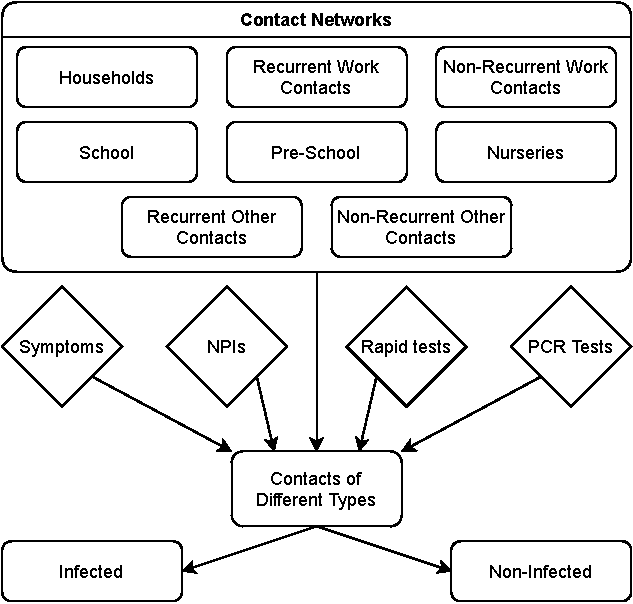
\includegraphics[width=\textwidth]{../figures/model-graph-top-left}
        \caption{{Model description}}
        \label{fig:broad_model_description}
    \end{subfigure}
    \hfill
    \begin{subfigure}[b]{0.425\textwidth}
        \centering
        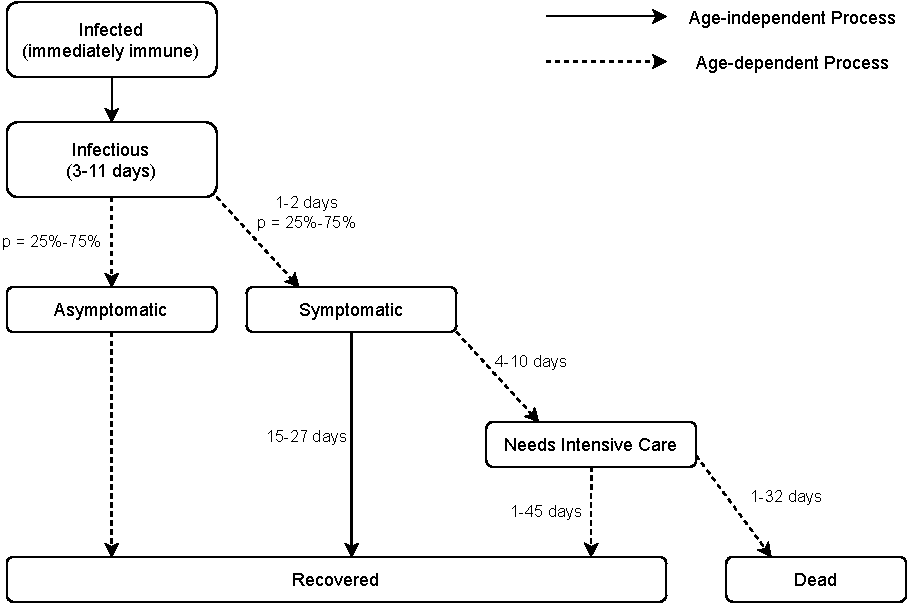
\includegraphics[width=\textwidth]{../figures/model-graph-top-right}
        \vskip4ex


        \caption{Disease progression}
        \label{fig:disease_progression}
    \end{subfigure}
    \vskip3ex
    \begin{subfigure}[b]{0.425\textwidth}
        \centering

        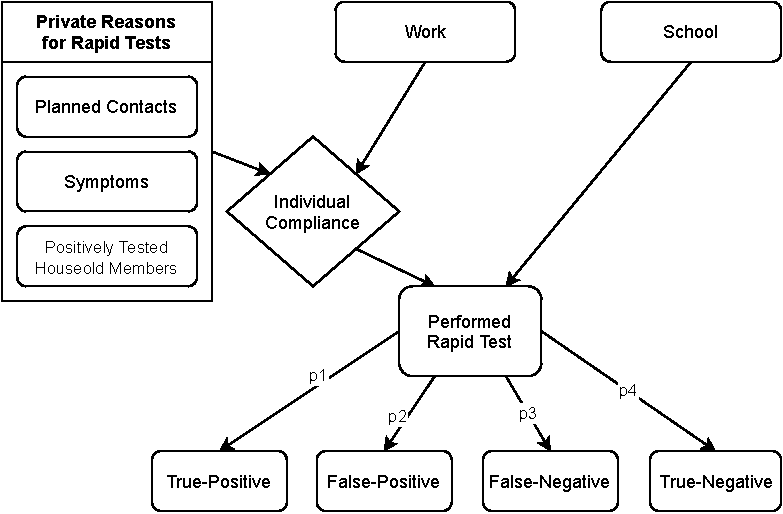
\includegraphics[width=\textwidth]{../figures/model-graph-bottom-left}
        \caption{{Model for antigen tests}}
        \label{fig:antigen_tests}
    \end{subfigure}
    \hfill
    \begin{subfigure}[b]{0.425\textwidth}
        \centering
        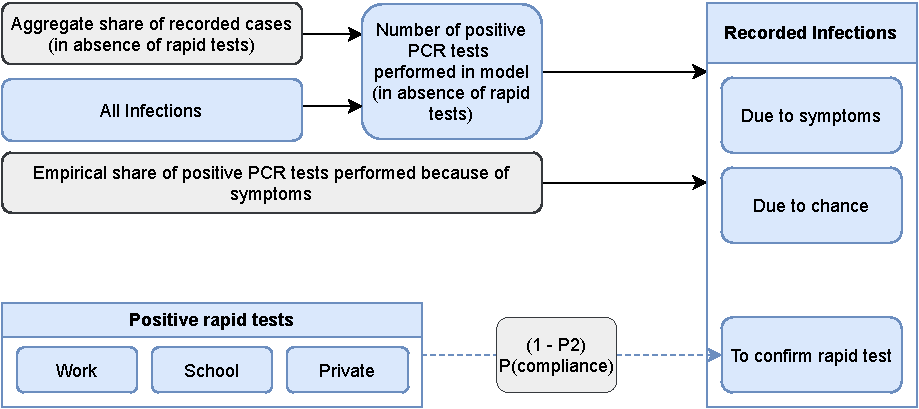
\includegraphics[width=\textwidth]{../figures/model-graph-bottom-right}
        \caption{{Model for undetected cases}}
        \label{fig:model_for_official_cases}
    \end{subfigure}

    \caption{Model description}
    \label{fig:model-description}

    \floatfoot{\noindent Note: ...}
\end{figure}

In our model, susceptibility to contracting the SARS-CoV-2 virus is dependent on age. A
possible infection progresses as shown in Figure~\ref{fig:disease_progression}. We
differentiate between an initial period of infection without being infectious or showing
symptoms, being infectious (presymptomatic or asymptomatic), showing symptoms, requiring
intensive care, and recovery or death as for example also modeled in \cite{Grimm2021}.
The probabilities of transitioning between these states depend on age; their duration is
random within intervals calibrated to medical literature (for a detailed description see
Section~\ref{sec:medical_params}). Conditional on the type of contact, infectiousness is
independent of age \citep{Jones2021}.

The model includes several other features, which are crucial to describe the evolution
of the pandemic in 2020-2021. New virus strains with different profiles regarding
infectiousness can be introduced. Agents may receive a vaccination. With a probability
of 75\% \citep{Hunter2021}, vaccinated agents become immune and they do not transmit the
virus \citep{Petter2021, LevineTiefenbrun2021, Pritchard2021}.\footnote{75\% is
    lower than what is usually reported for after the second dose of the Biontech/Pfizer
    vaccine, which is most commonly used in Germany. We choose it because our model neither
    includes booster shots, nor does it allow vaccinated individuals who became immune to
    transmit the disease\citep{Petter2021, LevineTiefenbrun2021, Pritchard2021}. If
    anything, these assumptions would overstate the effect of vaccines for our study period.
    This would be different if a large fraction of vaccinated individuals had received a
    second dose already.} During the vaccine roll-out, priority may depend on age and
occupation.

We include two types of tests. Polymerase chain reaction (PCR) tests directly reveal
whether an individual is infected or not. PCR tests require some days to be processed and
there are aggregate capacity constraints throughout. In contrast, rapid antigen tests
yield immediate results; after a phase-in period, all tests that are demanded will be
performed. Specificity and sensitivity of these tests is set according to data analyzed
in \cite{Bruemmer2021, Smith2021}; sensitivity depends on the timing of the test relative
to the start of infectiousness. Figure~\ref{fig:antigen_tests} shows our model for rapid
test demand. Schools may require students to be tested regularly. Rapid tests may be
offered by employers for on-site workers. Individuals may demand tests for private
reasons, which include having plans to meet other people\footnote{A positive test will
make them reduce their contacts; this is why tests impact the actual contacts in
Figure~\ref{fig:model-description}.}, showing symptoms of CoViD-19, and because a
household member tested positively for the virus. We endow each agent with an individual
compliance parameter. This parameter determines whether she takes up rapid tests offered
by employers or follows up on private reasons and whether she reduces her contacts if she
tests positive or develops symptoms. The thresholds are higher for tests in a private
setting than for tests at the workplace until mid April and then compliance because of
private reasons becomes higher than compliance at the workplace.

Modelling a population of agents according to actual demographic characteristics means
that we can use a wide array of data to identify and estimate the model's many
parameters.\footnote{See section~\ref{sec:data_and_parameters} of the supplementary
materials for an overview.} We can rely on contact diaries to get pre-pandemic
distributions of contacts for different contact types and their assortativity by age
group. Mobility data is used to model the reductions in work contacts. School and daycare
policies can be incorporated directly from official directives. Aggregate tests,
vaccinations and the prevalence of virus strains can be taken from official records. The
likelihood to receive a test offer or to take up a test offer and the share of
individuals that have ever taken a test or done weekly tests in the last month can be
calibrated from survey data.\comment[id=HM]{Anything else we need to
mention?}\comment[id=K]{I added some more that I think are worth mentioning.} We estimate
the infection probabilities\comment[id=HM]{need to be more precise here, cannot find in
Appendix}\comment[id=K]{I added \ref{subsec:infection_probs}.} that the simulated new
infections predict age- and region-specific time series.\comment[id=K]{We never directly
targeted the federal states if I remember it right. How large was their weight in the
criterion function @Janos?} However, the two sets of time series are not comparable
directly because not all cases will be recorded. We model the fraction of recorded cases
as depicted in Figure~\ref{fig:model_for_official_cases}.\comment[id=HM]{Add a sentence.}

The model is applied to the second and third wave of the CoViD-19 pandemic in Germany,
covering the period mid-September 2020 to the end of May 2021.
Figure~\ref{fig:pandemic_drivers_model_fit} describes the evolution of the pandemic and
of its drivers. The black line in Figure~\ref{fig:aggregated_fit} shows officially
recorded cases; the black line in Figure~\ref{fig:stringency_index} the Oxford Response
Stringency Index \citep{Hale2020}, which tracks the tightness of non-pharmaceutical
interventions. We transform the index so that lower values represent higher levels of
restrictions. A value of zero means all measures incorporated in the index are turned
on. The value 1 represents the situation in mid-September, with restrictions on
gatherings and public events, masking requirements, but open schools and workplaces. In
the seven weeks between mid September and early November, cases increased by a factor of
10. Restrictions were somewhat tightened in mid-October and again in early November. New
infections remained constant throughout November, before rising again in December, which
prompted the most stringent lockdown to this date. Schools and daycare centers were
closed again, so were customer-facing businesses except for grocery and drug stores.
From the peak of the second wave just before Christmas until the trough in mid-February,
newly detected cases decreased by almost three quarters. The third wave in the spring of
2021 is associated with the B.1.1.7 strain, which became dominant in March. See
Figure~\ref{fig:share_b117}. In early March, some NPIs were being relaxed; e.g.,
hairdressers and home improvement stores were allowed to open again to the public. There
were many changes in details of regulations afterwards, but they did not change the
stringency index.

\begin{figure}[!tp]
    \centering

    \begin{subfigure}[b]{0.475\textwidth}
        \centering
        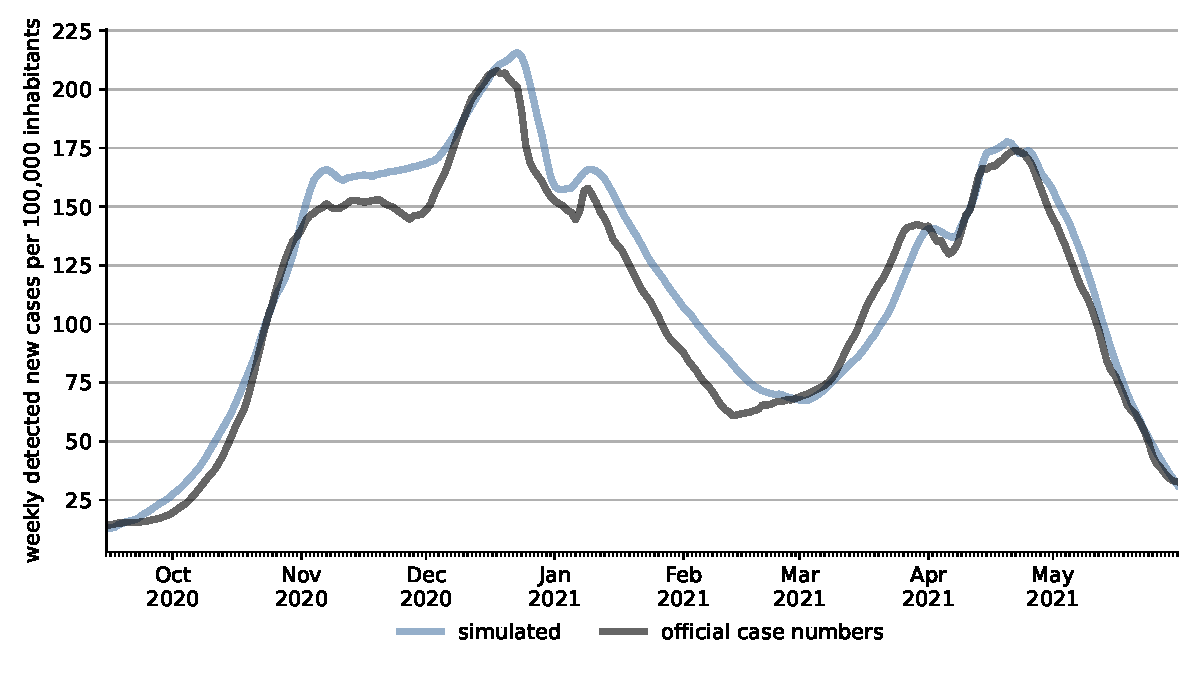
\includegraphics[width=\textwidth]{../figures/results/figures/scenario_comparisons/combined_fit/full_new_known_case}
        \caption{{Recorded cases: Empirical and simulated}}
        \label{fig:aggregated_fit}
    \end{subfigure}
    \hfill
    \begin{subfigure}[b]{0.475\textwidth}
        \centering
        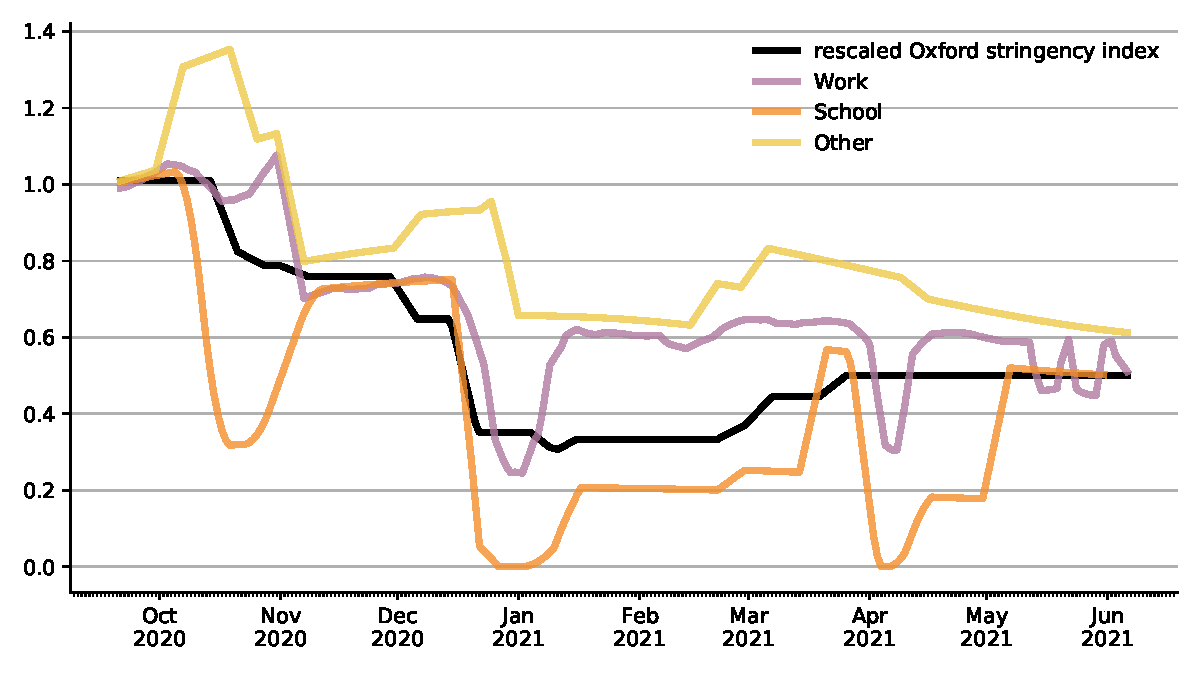
\includegraphics[width=\textwidth]{../figures/results/figures/data/stringency2_with_seasonality}

        \caption{{Stringency of NPIs and infectious contacts}}
        \label{fig:stringency_index}
    \end{subfigure}

    \vskip3ex

    \begin{subfigure}[b]{0.475\textwidth}
        \centering

        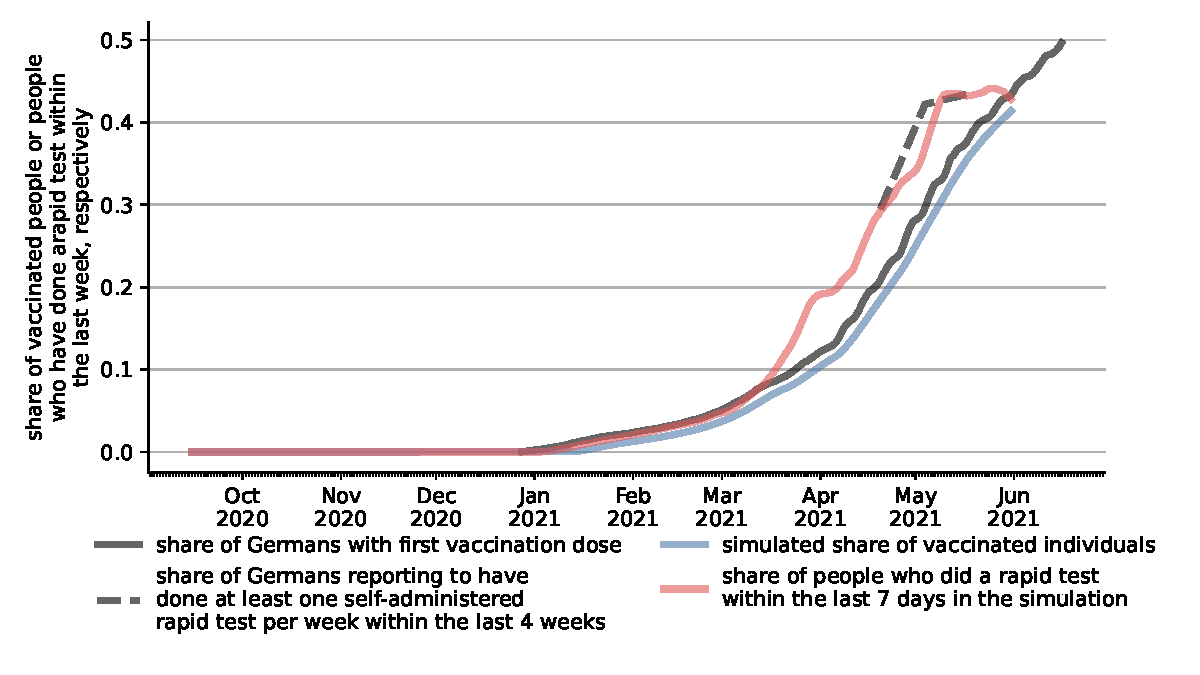
\includegraphics[width=\textwidth]{../figures/results/figures/scenario_comparisons/combined_fit/full_share_rapid_test_in_last_week_and_vaccinated}

        \caption{{Tests and vaccinations}}
        \label{fig:antigen_tests_vaccinations}
    \end{subfigure}
    \hfill
    \begin{subfigure}[b]{0.475\textwidth}
        \centering

        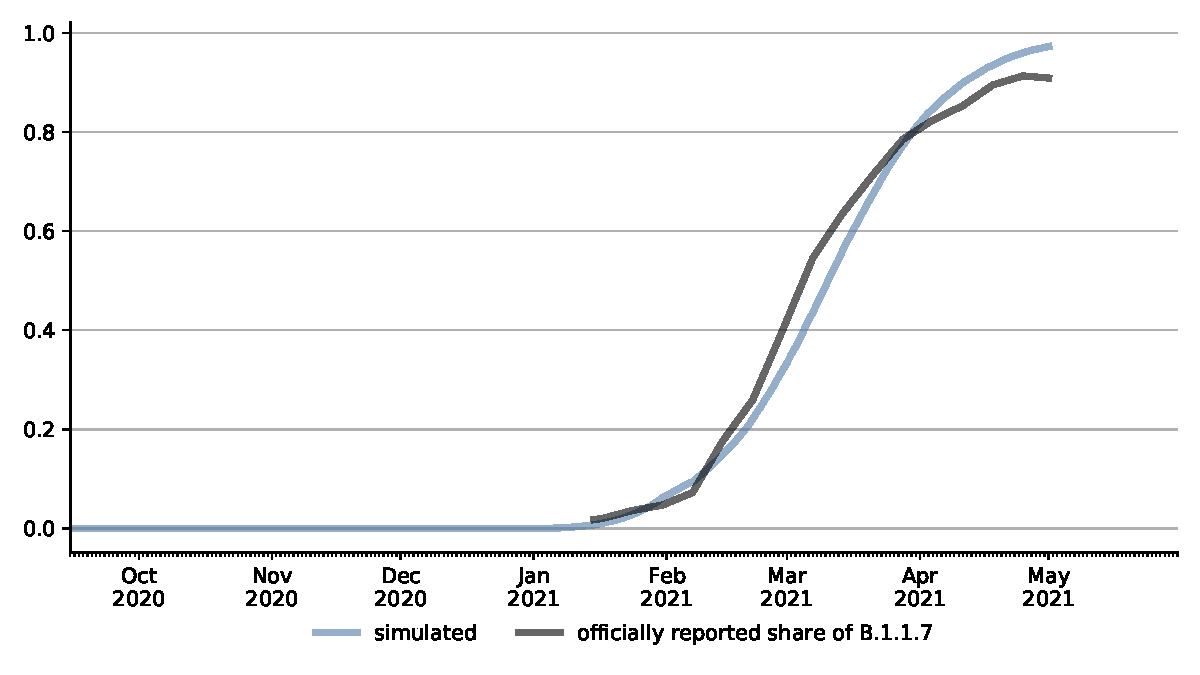
\includegraphics[width=\textwidth]{../figures/results/figures/scenario_comparisons/combined_fit/full_share_b117}

        \caption{Fraction of B.1.1.7 strain}
        \label{fig:share_b117}
    \end{subfigure}

    \caption{Evolution of the pandemic, its drivers, and model fit, September 2020 to May 2021}
    \label{fig:pandemic_drivers_model_fit}

    \floatfoot{\noindent Note: All aggregates; See S.XXX for statistics by age group and
        by geographical region. Also more disaggregated data.

        Sources: ...}

\end{figure}

By this time, the set of policy instruments had become much more diverse. Around the
turn of the year, the first people were vaccinated with a focus on older age groups and
medical personnel (Figure~\ref{fig:antigen_tests_vaccinations}. By the end of May, just
over 40\% had received at least one dose of a vaccine. Around the same time, rapid tests
started to replace regular PCR tests for staff in many medical and nursing facilities.
These had to be administered by medical doctors or in pharmacies. At-home tests approved
by authorities became available in mid-March, rapid test centers were opened and one
test per person and week was made available free of charge. Depending on the state,
customers were only allowed to enter certain stores with a recent negative rapid test
result. These developments are characteristic of many countries: The initial focus on
NPIs to slow the spread of the disease has been accompanied by vaccines and a growing
acceptance and use of rapid tests. At broadly similar points in time, novel strains of
the virus have started to pose additional challenges.

We draw simulated samples of agents from the distribution of recorded infections in
September 2020 and use the model to predict recorded infection rates until the end of
May 2021. See Supplementary Materials~\ref{sec:data_and_parameters} and \ref{sec:model}
for detailed descriptions of the data and the model, respectively. The blue line in
Figure~\ref{fig:aggregated_fit} shows our model's predictions are very close to
officially recorded cases in the aggregate. This is also true for infections by age and
geographical region, which are shown in the supplementary materials
(Figures~\ref{fig:age_group_fit} and \ref{fig:state_fit}, respectively).

The effects of various mechanisms can be disentangled due to the distinct temporal
variation in the drivers of the pandemic. Next to the stringency index, the three lines
in Figure~\ref{fig:stringency_index} summarize how contact reductions, increased hygiene
regulations, and seasonality evolved since early September for each of the three broad
contact networks. For example, a value of 0.75 for the work multiplier means that if the
environment was the same as in September (levels of infection rates, no rapid tests or
vaccinations, only the wildtype virus present), infections at the workplace would be
reduced by 25\%. The lines show the product of the effect of contact reductions,
increased hygiene regulations, and seasonality. See Appendix~\comment[id=HM]{Reference}
for separate plots of the three factors. Two aspects are particularly interesting.
First, all lines broadly follow the stringency index and they would do so even more if
we left out seasonality and school vacations (roughly the last two weeks of October, two
weeks each around Christmas and Easter, and some days in late May). Second, the most
stringent regulations are associated with the period of strong decreases in new
infections between late December 2020 and mid-February 2021. The reversal of the trend
is associated with he spread of the B.1.1.7 variant. The steep drop in recorded cases
during May 2021 is associated with at least weekly rapid tests to around 42~percent of
the population, a vaccination rate that rose from 28\% to 43\%, and mostly seasonality
impacting a fall in the relative infectiousness of contacts outside of work and school.

In order to better understand the contributios  of rapid tests, vaccinations, and of
seasonality on the evolution of infections in 2021,
Figure~\ref{fig:2021_scenarios_broad} considers various scenarios. NPIs are always the
same as in the baseline scenario. Figure~\ref{fig:2021_scenarios_recorded} shows the
model fit (the blue line, same as in Figure~\ref{fig:aggregated_fit}), a scenario
without any of the three factors (red line), and three scenarios turning these factors
off one by one. Figure~\ref{fig:2021_scenarios_newly_infected} does the same for total
infections in the model. Figure~\ref{fig:2021_scenarios_decomposition} employs Shapley
values to decompose the difference in total infections between the scenario without any
of the three factors and our main specification.

\begin{figure}[!tp]
    \centering

    \begin{subfigure}[b]{0.475\textwidth}
        \centering
        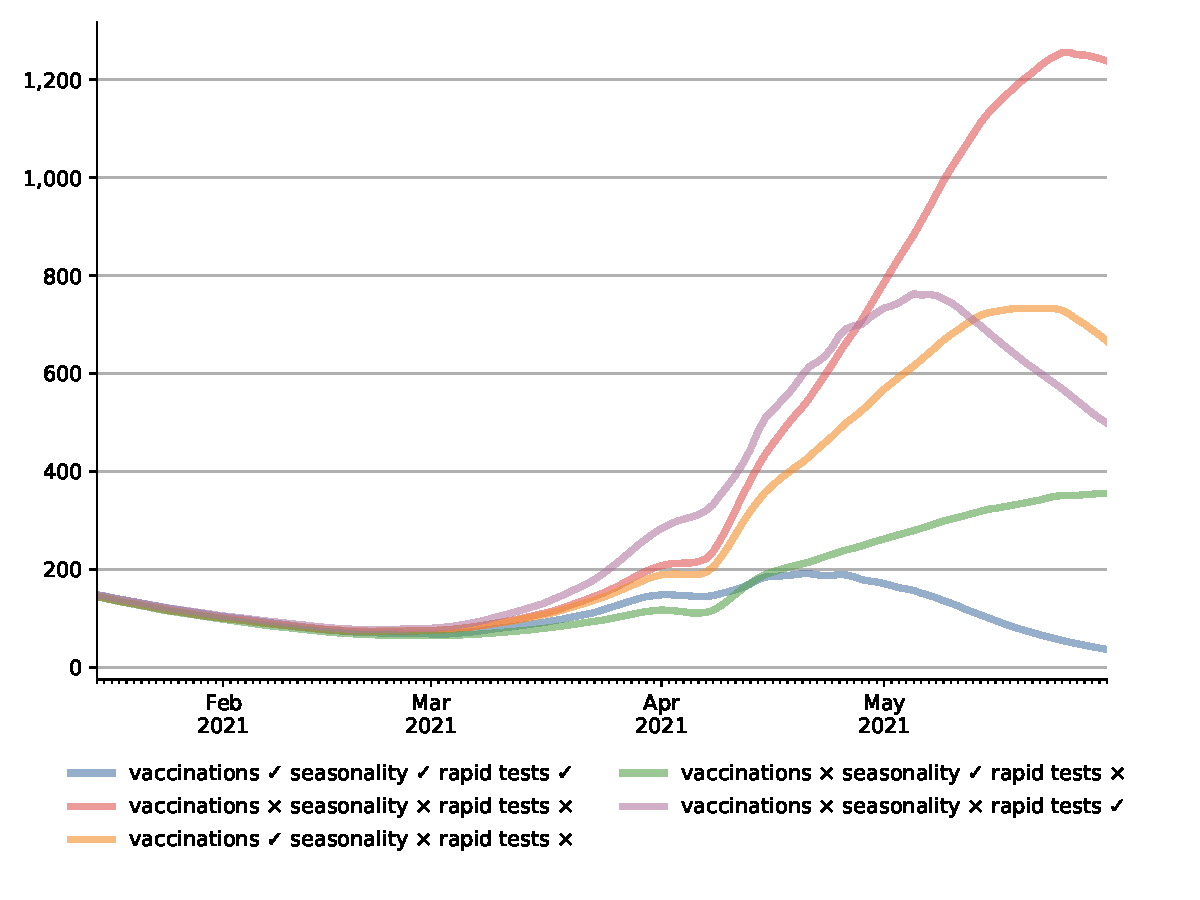
\includegraphics[width=\textwidth]{../figures/results/figures/scenario_comparisons/effect_of_channels_on_pessimistic_scenario/full_new_known_case}
        \caption{{Recorded cases: 2021 scenarios}}
        \label{fig:2021_scenarios_recorded}
    \end{subfigure}
    \hfill
    \begin{subfigure}[b]{0.475\textwidth}
        \centering
        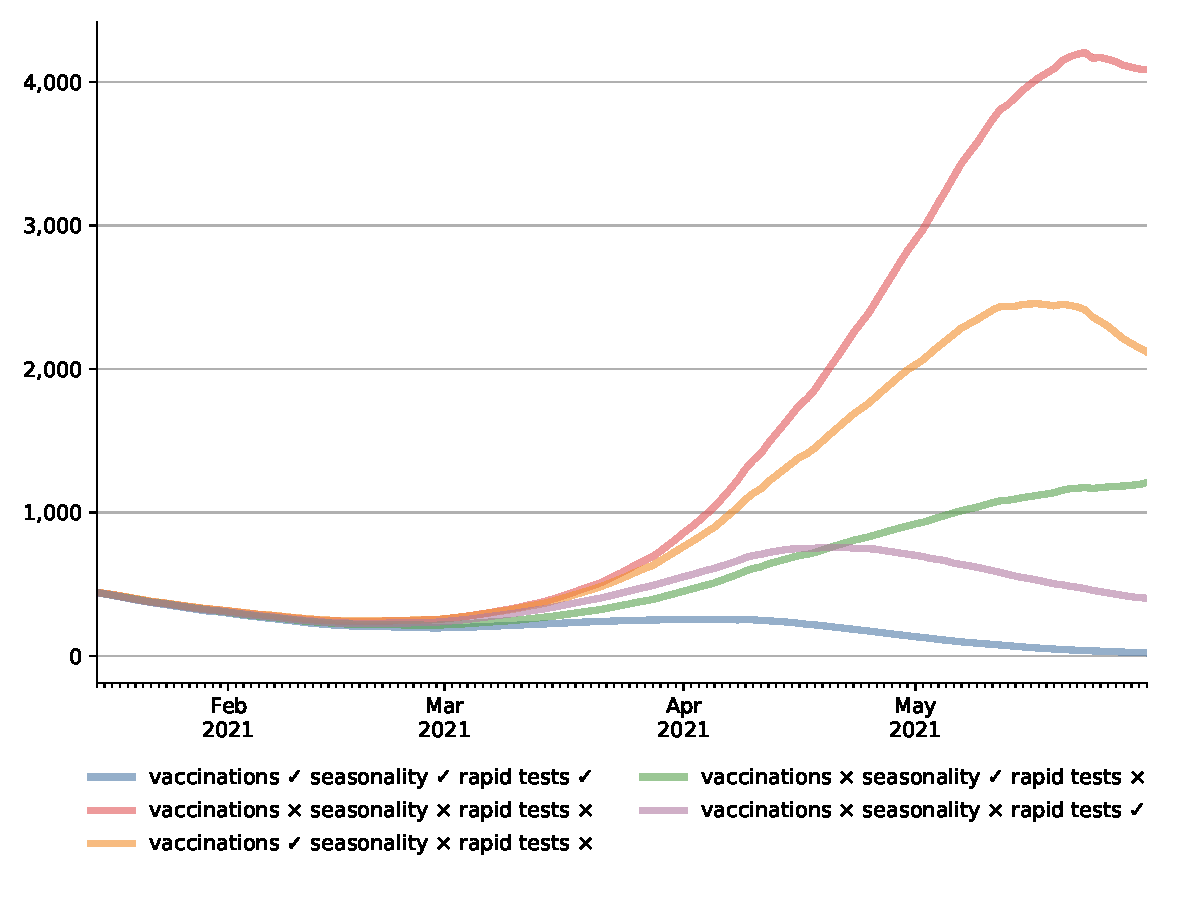
\includegraphics[width=\textwidth]{../figures/results/figures/scenario_comparisons/effect_of_channels_on_pessimistic_scenario/full_newly_infected}
        \caption{{Total cases: 2021 scenarios}}
        \label{fig:2021_scenarios_newly_infected}
    \end{subfigure}

    \begin{subfigure}[b]{0.475\textwidth}
        \centering
        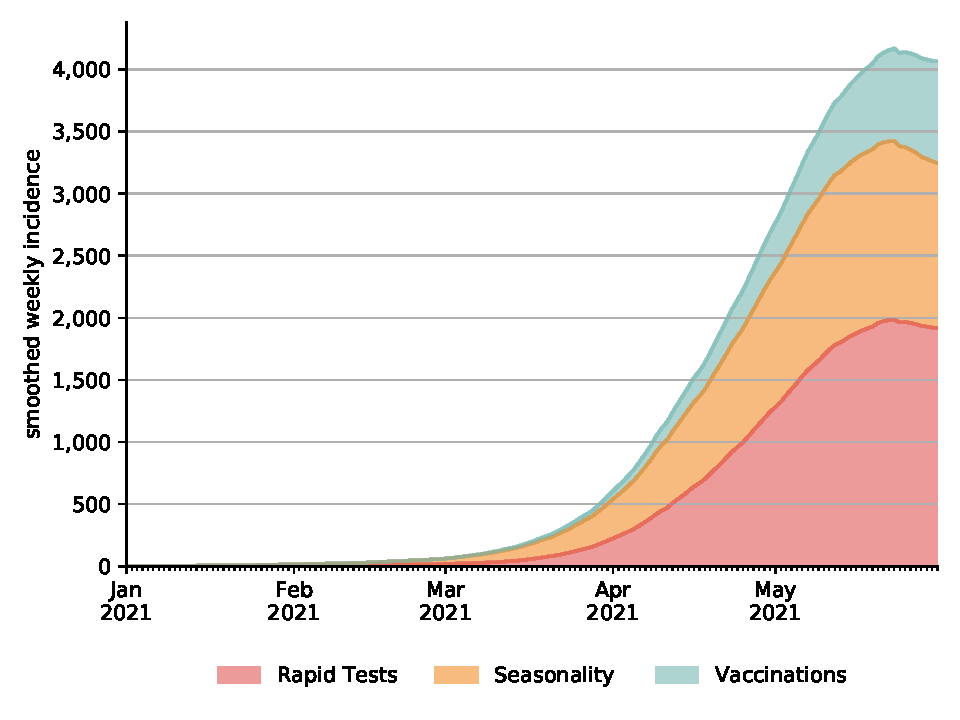
\includegraphics[width=\textwidth]{../figures/results/figures/full_decomposition_channels_area}
        % 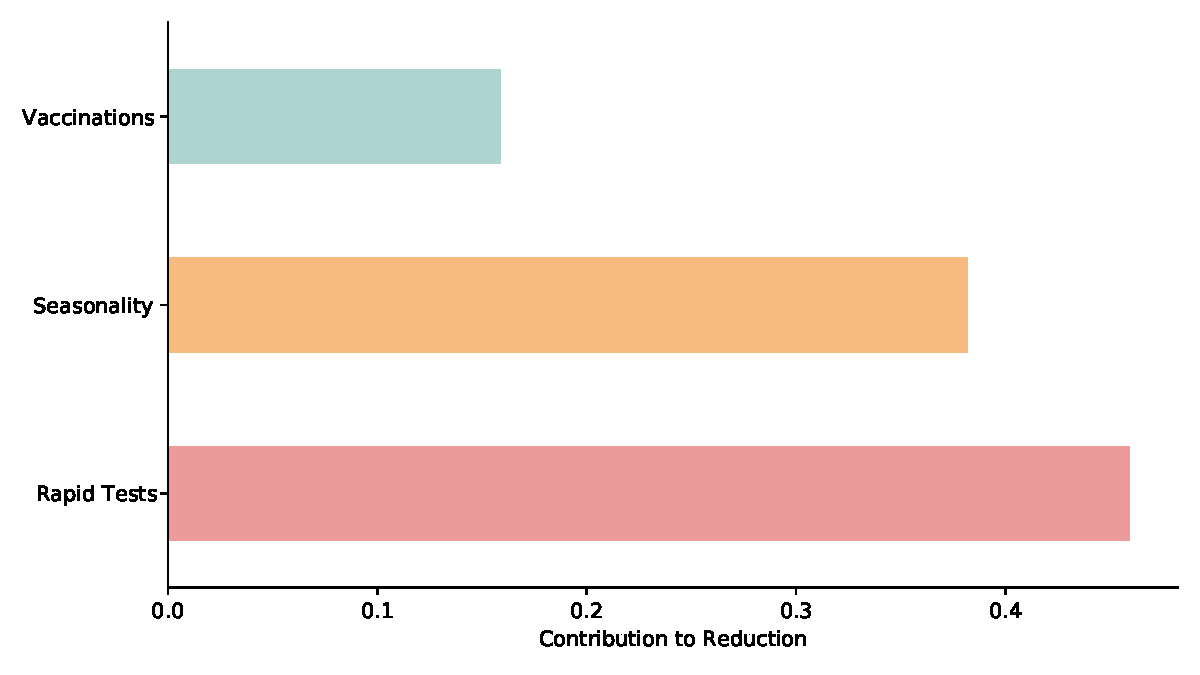
\includegraphics[width=\textwidth]{../figures/results/figures/full_decomposition_channels_bar}
        \caption{Decomposition of the difference between the scenario without any of the
            three factors and the main scenario in
            Figure~\ref{fig:2021_scenarios_newly_infected}.}
        \label{fig:2021_scenarios_decomposition}
    \end{subfigure}
    \hfill
    \begin{subfigure}[b]{0.475\textwidth}
        \centering
        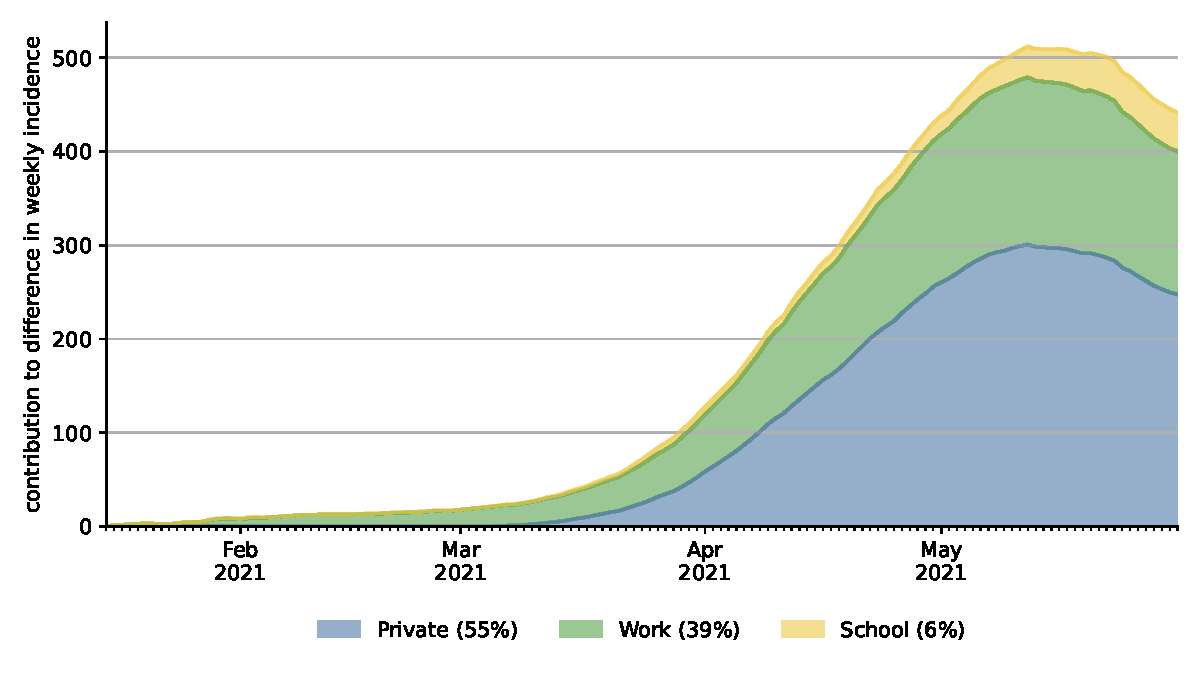
\includegraphics[width=\textwidth]{../figures/results/figures/full_decomposition_rapid_tests_area}
        % 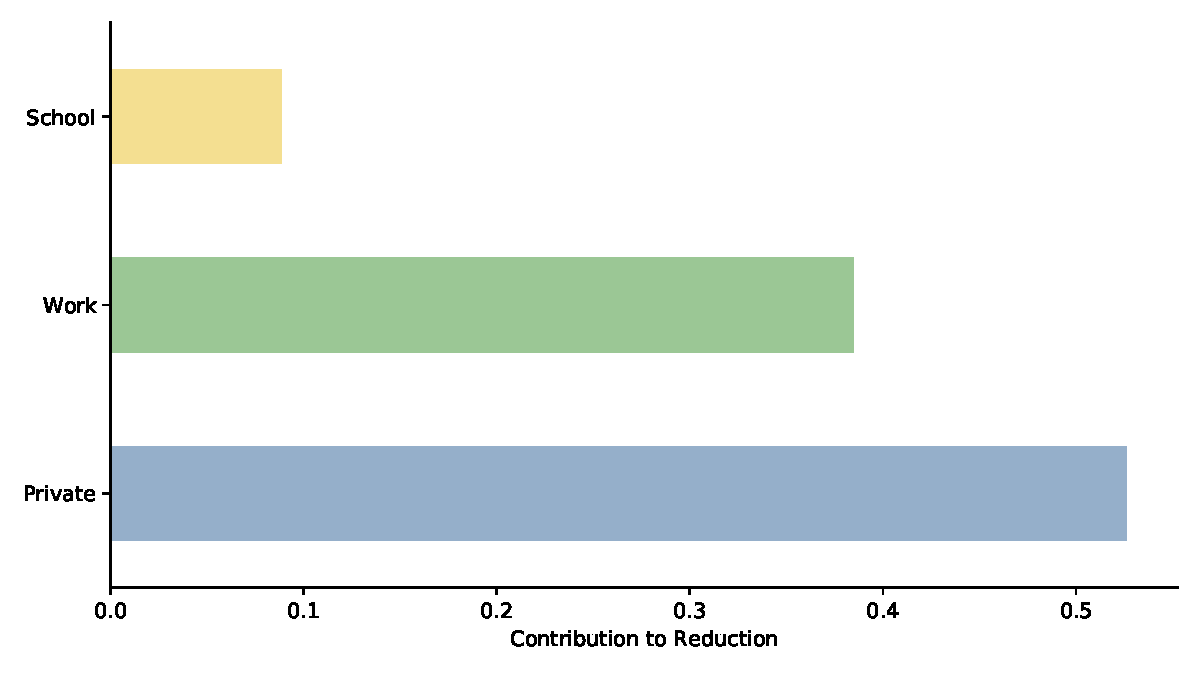
\includegraphics[width=\textwidth]{../figures/results/figures/full_decomposition_rapid_tests_bar}
        \caption{Decomposition of the difference between the scenario without rapid
            tests and the main scenario in Figure~\ref{fig:2021_scenarios_newly_infected}.}
        \label{fig:2021_scenarios_decomposition_tests}
    \end{subfigure}

    \caption{The effect of different interventions on recorded and actual infections}
    \label{fig:2021_scenarios_broad}

    \floatfoot{\noindent Note: All aggregates; See S.XXX for statistics by age group and
        by geographical region.

        The decomposition is based on Shapley values where the individual contribution
        of a channel is its average contribution over different sizes of coalitions
        (combinations with other channels). The individual contribution to a coalition
        is the difference between the effect size of the coalition with the particular
        channel and without.}
\end{figure}

Until mid-March, there is no visible difference between the different scenarios.
Seasonality hardly changes, and only few vaccinations or rapid tests were administered.
Even thereafter, the effect of the vaccination campaign is surprisingly small at first
sight. Whether considering recorded or total infections with only one channel active,
the final level is always the highest in case of the vaccination campaign (orange
lines). The Shapley value decomposition shows that vaccinations contribute about 15\% to
the cumulative difference between scenarios. Reasons for this are the slow start---it
took until March~24th until 10\% of the population had received their first vaccination,
the 20\% mark was reached on April 19th---and the focus on older individuals. These
groups contribute less to the spread of the disease than others due to a lower number of
contacts, see Supplementary Material~\ref{subsec:contacts_by_age}. It is important to
note that the initial focus of the campaign was to prevent deaths and severe disease;
the case fatality was rate considerably lower during the third wave when compared to the
second (4.4\% between October and February and 1.4\% between March and June). It is
important to note that by the end of our study period, when first-dose vaccination rates
reached around 40\% of the population, the numbers of new cases would have started to
decline.

Seasonality has a large effect in slowing the spread of SARS-CoV-2. By May 31, both
observed and recorded cases would be reduced by a factor of four if only seasonality
mattered. However, in this period, cases would have kept on rising throughout, just at a
much lower pace. Nevertheless, we estimate it to be a quantitatively important factor
determining the evolution of the pandemic, explaining most of the early changes and
almost 40\% of the cumulative difference by the end of May.

The largest effect---almost one half when considering the decompositions---comes from
rapid testing. Here, it is crucial to differentiate between recorded cases and actual
cases. Additional testing means that infections become known, which would otherwise
remain undetected. Figure~\ref{fig:2021_scenarios_recorded} shows that this means that
until late April, recorded cases are higher than in the scenario where none of the three
mechanisms is turned on. Compared to the scenario with vaccinations only, this point is
reached around mid-May and it would be June for the comparison with the seasonality-only
scenario. The effect on total cases, however, is visible immediately. Despite the fact
that only a small fraction of the population performed weekly rapid tests in
March\footnote{X\% in the model; 27\% of respondents to the COSMO study reported in
    early March that they \textit{ever} did a rapid test)}\comment[id=HM]{Put in}, new
infections on April 1 would be reduced by 53\% relative to the scenario without
vaccinations, rapid tests, or seasonality.

So why is rapid testing so effective? In order to shed more light on this question,
Figure~\ref{fig:2021_scenarios_decomposition_tests} decomposes the difference in the
scenario without rapid tests only (purple line in
Figure~\ref{fig:2021_scenarios_newly_infected}) and the main specification into the
three channels for rapid tests. Tests for pupils have the smallest effect, which is
largely explained by the relatively small number of students (XXM pupils vs. YYM
workers)\comment[id=HM]{fill in} and the fact that schools did not operate at full
capacity during our period of study. Almost 40\% come from tests at the workplace.
Despite the fact that we phase rapid tests for private reasons are phased in only late,
they make up for more than half of the total effect.

\comment[id=HM]{How many tests are actually performed along each of the three dimensions? Could this be a quantity story rather than the directed testing story I am making up here as wishful thinking?}

The reason lies in the fact that a substantial share of these tests is driven by an
elevated probability to carry the virus, i.e., showing symptoms of CoViD-19 or following
up on a positive test of a household member. The latter is essentially a form of contact
tracing, which has been shown to be very effective.\comment[id=HM]{cite Priesemann
paper, others?} This is also the reason for why the number of tests performed fall at
the very end of our study period. Falling infection rates mean that there are fewer
events triggering private test demand.
\comment[id=HM]{Positive rates along the three channels might be nice here, if previous comment is not a quant story}
\comment[id=HM]{I think there is a story in here about risk conditional on past exposure vs. prospective risk in gatherings, but it is too late to work through it. We might just want to calculate the probabilities.}

Two of the most contentious NPIs concern schools and mandates to work from home. In many
countries, schools switched to remote instruction during the first wave, so did Germany.
After the summer break, they were operating at full capacity with increased hygiene
measures, before being closed again from mid-December on. Some states started opening
them gradually in late February, but usual operaton was not back until the beginning of
June. Figure~\ref{fig:school_scenarios} shows the effects of different policies regarding school starting at Easter, a point where rapid tests had become widely available. 

In light of the large negative effects school closures have on children and
parents\comment[id=HM]{need to cite a couple of poor learning outcomes / mental health
papers. There must be well-published ones}---and in particular on those with low
socio-economic status---the results in

Effects:
\begin{itemize}
    \item Schools were essentially closed
    \item What are the different $R_t$-values? In no-test scenario and $R_t>1$, might be
          worth chopping off 0.05 or whatever that might be?
    \item With tests it is really hard to make a case for that
\end{itemize}

Alternative:
\begin{itemize}
    \item Germany quite lenient on home office relative to other countries (employer had
          to allow)
    \item Testing: Rapid tests are cheap (less than 1\euro), just a nuisance.
\end{itemize}

Results
\begin{itemize}
    \item Advantage of testing in both cases: Recurrent. Small cost relative to other
          stuff. Certain publicness.
    \item Mandatory tests: Screening effect for hard-to-reach populations (do not
          consider in this paper, also due to poor data in DE)
\end{itemize}


\begin{figure}[!tp]
    \centering

    \begin{subfigure}[b]{0.475\textwidth}
        \centering
        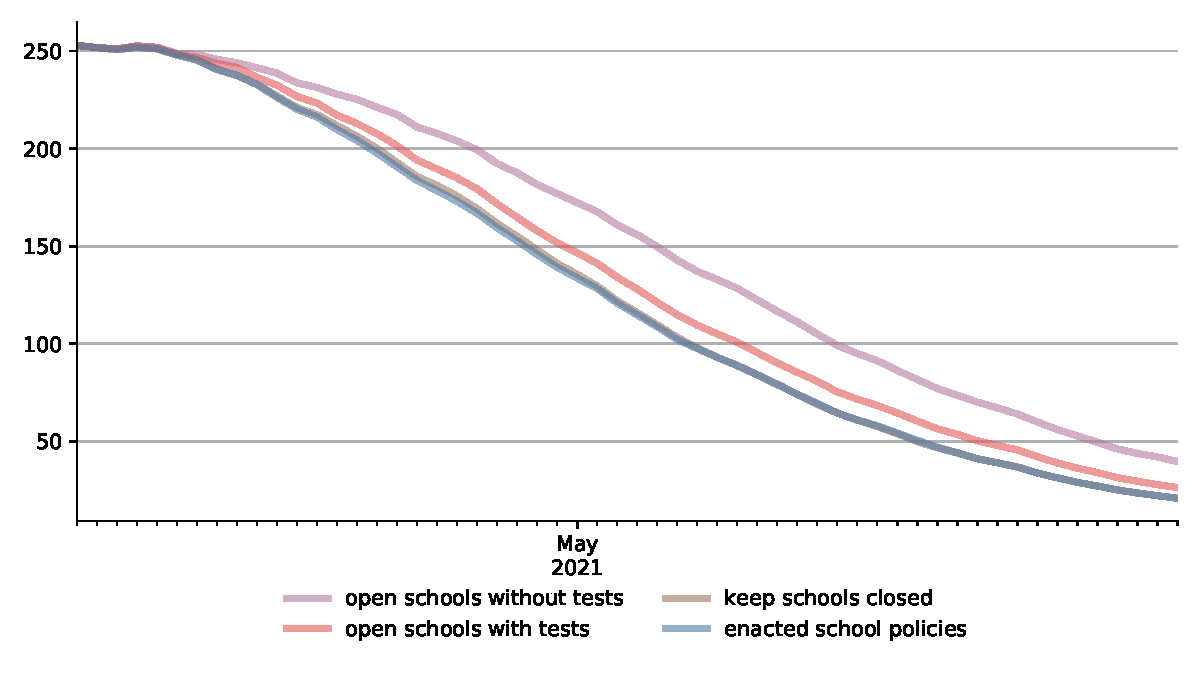
\includegraphics[width=0.9 \textwidth]{../figures/results/figures/scenario_comparisons/school_scenarios/full_newly_infected}
        \caption{{Effects of different schooling scenarios}}
        \label{fig:school_scenarios}
    \end{subfigure}
    \hfill
    \begin{subfigure}[b]{0.475\textwidth}
        \centering
        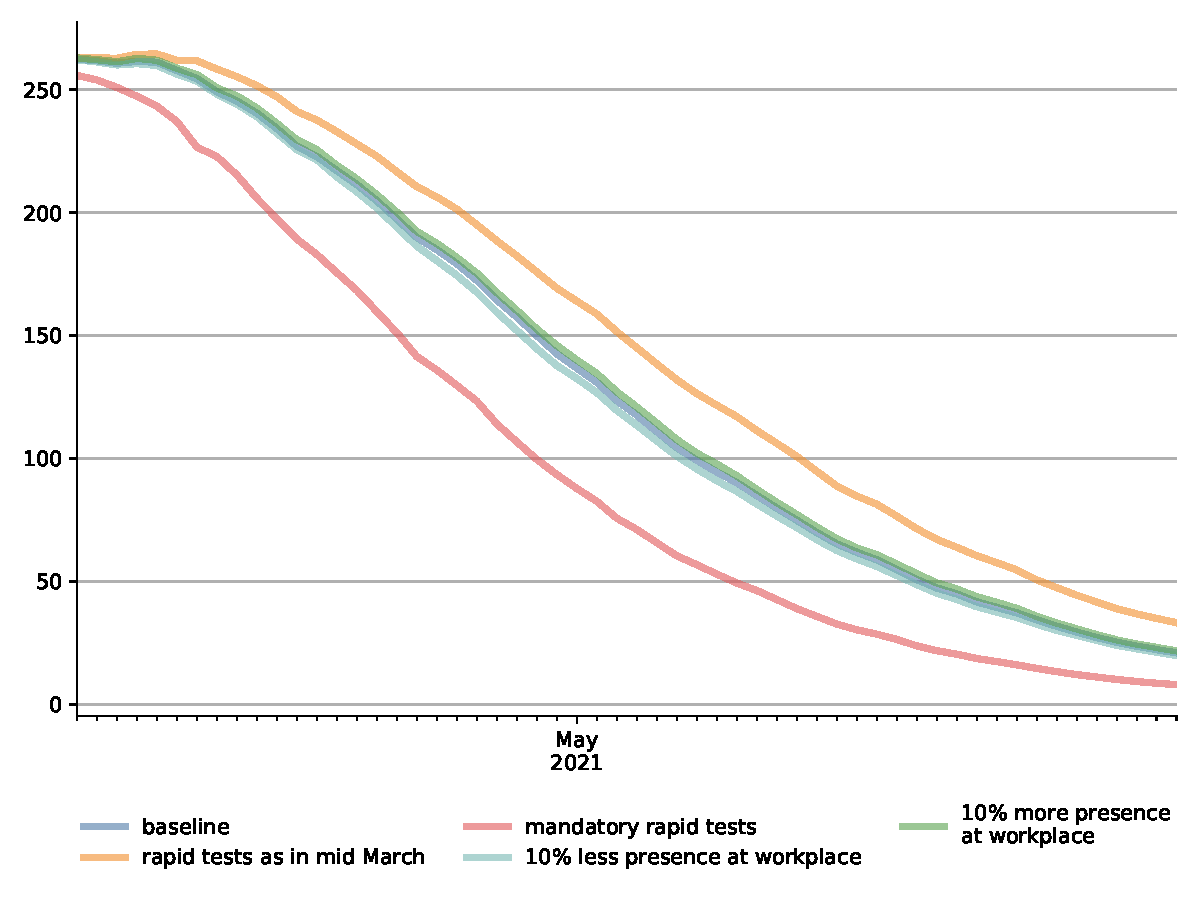
\includegraphics[width=0.9 \textwidth]{../figures/results/figures/scenario_comparisons/new_work_scenarios/full_newly_infected}
        \caption{{Effects of different work scenarios}}
        \label{fig:workplace_scenarios}
    \end{subfigure}
    \vskip3ex

    \caption{Effects of different scenarios for policies regarding schools and workplaces.}
    \label{fig:school_workplace_scenarios}

    \floatfoot{\noindent Note: Interventions start at Easter because there were no
        capacity constraints for rapid tests afterwards.}

\end{figure}


\phantomsection % Needed for the bibliography bookmark to point to the correct page

\begin{refcontext}[sorting=nyt]  % Sort BIBLIOGRAPHY by alphabet (while CITATIONS are sorted by year)
\printbibliography[heading=bibintoc]
\end{refcontext}

\clearpage

\begin{center}
    {
        \Large 
        Supplementary Material for\\[2ex]
    
        \textbf{\papertitle}
    }
    \vskip4ex
    {
        \large
        Janoś Gabler,
        
        Tobias Raabe,
        
        Klara Röhrl,
        
        Hans-Martin von Gaudecker

    }
\end{center}

\tableofcontents

\clearpage

\begin{appendices}
    \begin{refsection}

    \section{Data and Parameters}
\label{sec:data_and_parameters}

The model is described by a large number of parameters that govern the number of
contacts a person has, the likelihood of becoming infected on each contact, the
likelihood of developing light or strong symptoms or even dying from the disease as well
as the duration each stage of the disease takes.

Most of these parameters can be calibrated from existing datasets or the medical
literature or calibrated from surveys and empirical datasets.

\subsection{Medical Parameters}

This section discusses the medical parameters used in the model, their sources and how we arrived at the distributions used in the model.\footnotemark

\footnotetext{Additional information can be found in the \href{https://sid-dev.readthedocs.io/en/latest/reference_guides/epi_params.html}{online documentation}.}


\subsubsection{Length of Presymptomatic Stage / Incubation Period}


Estimates of the incubation period usually give a range from 2 to 12 days. A meta analysis by \citet{McAloon2020} comes to the conclusion that ``The incubation period distribution may be modeled with a lognormal distribution with pooled $\mu$ and $\sigma$ parameters (95\% CIs) of 1.63 (95\% CI 1.51 to 1.75) and 0.50 (95\% CI 0.46 to 0.55), respectively.'' For simplicity we discretize this distribution into four bins.


\subsubsection{Begin of Infectiousness}

The period between infection and onset of infectiousness is called latent or latency period. However, the latency period is rarely given in epidemiological reports on Covid-19. Instead, scientists and agencies usually report the incubation period, the period from infection to the onset of symptoms. A few studies used measurements of virus shedding to estimate infectiousness during the course of the disease. When measurements started before the onset of symptoms the development of the viral load before symptoms gives us an indication of number of days between the onset of infectiousness and symptoms.

The European Centre for Disease Prevention and Control estimates that people become infectious between one and two days before the symptoms set in. This is similar to \citet{He2020} who estimate this to take 2.3 days and is in line with \citet{Peak2020}.

Given these numbers and the length of the incubation period we can calculate the latency period for symptomatic people. To our knowledge no estimates for the latency period of asymptomatic cases of COVID-19 exist. We assume it to be the same for symptomatic and asymptomatic cases.

Thus, we arrive at the following distribution for latency periods: 40\% have one day. 35\% have two days. 20\% have three days and 5\% have 5 days.


\subsubsection{Duration of Infectiousness}

We assume that the duration of infectiousness is the same for both symptomatic and asymptomatic individuals as evidence suggests little differences in the transmission rates of SARS-CoV-2 virus between symptomatic and asymptomatic patients (\citet{Yin2020}) and that the viral load between symptomatic and asymptomatic individuals are similar (\citet{Zou2020}, \citet{Byrne2020}, \citet{Singanayagam2020}).

Our distribution of the duration of infectiousness is based on \citet{Byrne2020}.

For symptomatic cases they arrive at 0-5 days before symptom onset (figure 2) and 3-8 days of infectiousness afterwards.\footnote{Viral loads may be detected much later but 8 days seems to be the time after which most people are culture negative, as also reported by \citet{Singanayagam2020}} Thus, we arrive at 0 to 13 days as the range for infectiousness among individuals who become symptomatic (see also figure 5). This duration range is very much in line with the meta-analysis’ reported evidence for asymptomatic individuals (see their figure 1). Thus, we arrive at 0 to 13 days as the range for infectiousness among individuals who become symptomatic. This duration range is very much in line with the meta-analysis' reported evidence for asymptomatic individuals.

Following this evidence we assume the following discretized distribution of the infectiousness period: 10\% of individuals are infectious for three days, 25\% for five days, another 25\% for seven days, 20\% for nine days and 20\% for eleven days.


\subsubsection{Duration of Symptoms}

We use the duration to recovery of mild and moderate cases reported by \cite[Figure~S3, Panel~2]{Bi2020} for the duration of symptoms for asymptomatic and non-ICU requiring symptomatic cases.

We collapse the data to the following distribution: 10\% recover after 15 days and 30\% require 18, 22 or 27 days respectively.

These numbers are only used for mild cases. We do not disaggregate by age. Note that the length of symptoms is not very important in our model given that individuals stop being infectious before their symptoms cease.


\subsubsection{Time from Symptom Onset to Admission to ICU}

The data on how many percent of symptomatic patients will require ICU is pretty thin. We rely on data by the US CDC (\citet{Stokes2020}) and \href{https://github.com/BDI-pathogens/OpenABM-Covid19/blob/572e24ca2dbf7153789a92ad3a27e4c515d0e576/documentation/parameters/parameter_dictionary.md}{the OpenABM-Project}. Table~\ref{tab:symptomatic-to-ICU} shows our derivations for the probabilities of requiring intensive care per age group.

\begin{table}[tb]
    \caption{Shares of symptomatic patients who will require ICU care by age groups.}
    \label{tab:symptomatic-to-ICU}
    \centering

    \begin{tabular}{ll}
        \toprule
        Age Group & Share \\
        \midrule
        0-9 & 0.00005 \\
        10-19 & 0.00030 \\
        20-29 & 0.00075 \\
        30-39 & 0.00345 \\
        40-49 & 0.01380 \\
        50-59 & 0.03404 \\
        60-69 & 0.10138 \\
        70-79 & 0.16891 \\
        80-100 & 0.26871 \\
        \bottomrule
    \end{tabular}

    \tablenotes{The data is taken from \citet{Stokes2020} and \href{https://github.com/BDI-pathogens/OpenABM-Covid19/blob/572e24ca2dbf7153789a92ad3a27e4c515d0e576/documentation/parameters/parameter_dictionary.md}{the OpenABM-Project}.}

\end{table}

For those who will require intensive care we follow \citet{Chen2020} who estimate the time from symptom onset to ICU admission as 8.5 $\pm$ 4 days.

This aligns well with numbers reported for the time from first symptoms to hospitalization: \citet{Gaythorpe2020} report a mean of 5.76 with a standard deviation of 4. This is also in line with the durations collected by \href{https://www.rki.de/DE/Content/InfAZ/N/Neuartiges_Coronavirus/Steckbrief.html#doc13776792bodyText16}{the Robert Koch Institut}.

We assume that the time between symptom onset and ICU takes 4, 6, 8 or 10 days with equal probabilities. These times mostly matter for the ICU capacities.


\subsubsection{Death and Recovery from ICU}

We take the survival probabilities and time to death and time until recovery from intensive care from the \href{https://tinyurl.com/y5owhyts}{OpenABM Project}.

They report time until death to have a mean of 11.74 days and a standard deviation of 8.79 days. Approximating this with the normal distribution, we have nearly 10\% probability mass below 0. We use it nevertheless as several other distributions (such as chi squared and uniform) were unable to match the variance.
Discretizing this leads to 41\% of individuals who die from Covid-19 to die after one day in intensive care. 22\% day after 12 days, 29\% after 20 days and 7\% after 32 days. Again, we rescale this for every age group among those that will not survive.

They report time until recovery to have a mean of 18.8 days and a standard deviation of 12.21 days. Approximating this with the normal distribution, we have over 5\% probability mass below 0. Discretizing this of those who recover in intensive care 22\% do so after one day, 30\% after 15 days, 28\% after 25 days and 18\% after 45 days.


\subsection{Number of Contacts}
\label{sub:number_of_contacts}

We calibrate the parameters for the predicted numbers of contacts from contact diaries
of over 2000 individuals from Germany, Belgium, the Netherlands and Luxembourg
\citep{Mossong2008}. Each contact diary contains all contacts an individual had
throughout one day, including information on the other person (such as age and gender)
and information on the contact. Importantly, for each contact individuals entered of
which type the contact (school, leisure, work etc.) was and how frequent the contact
with the other person is.

Simplifying the number of contacts, we arrive at the following distributions of the
numbers of contacts by contact type.

\begin{figure}
    \centering
    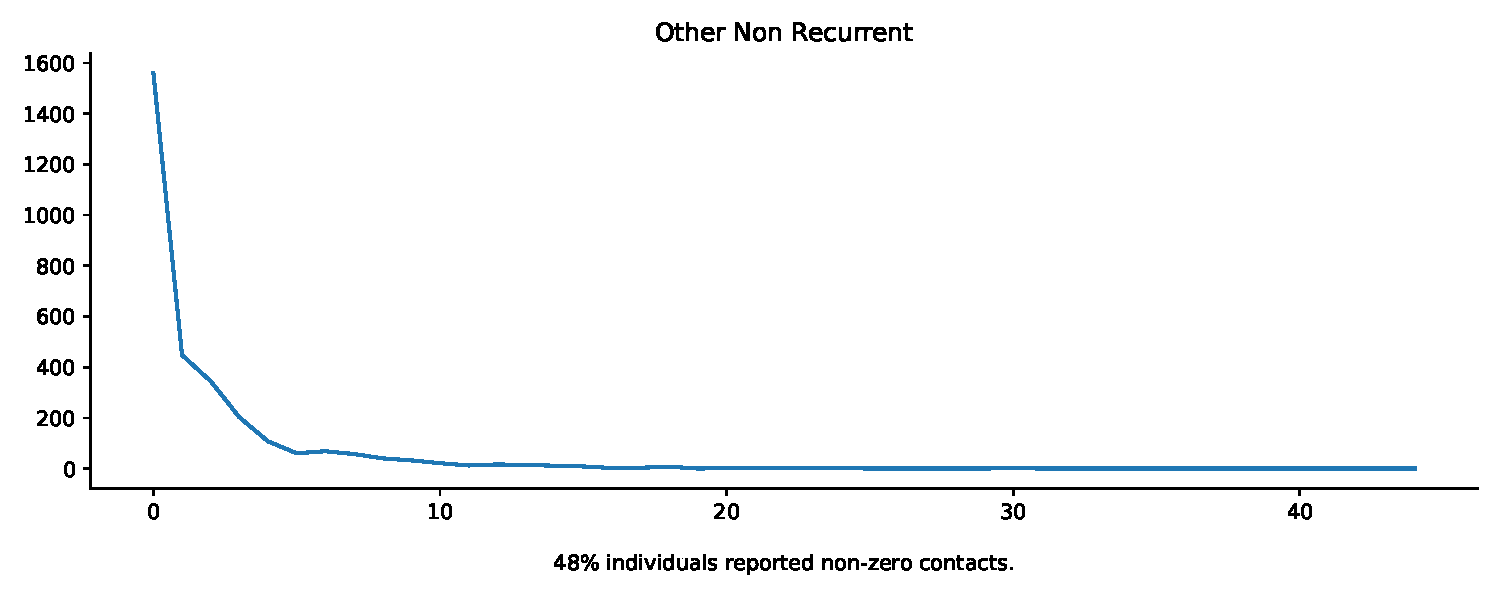
\includegraphics[width=\textwidth]{../figures/results/figures/data/distributions_of_the_number_of_contacts/other_non_recurrent}
    \caption{Number of Non Recurrent Other Contacts}
    \label{n_contacts_other_non_recurrent}
    \floatfoot{\noindent In the model it is sampled every day which of these numbers of
    contacts a person is planned to have. Note that the contact diaries include such high
    values that super spreading events are well possible in our model. The planned number
    of contacts is reduced by policies, seasonality and individual responses to events
    such as receiving a positive rapid test to the number of actual contacts with
    transmission potential. Other contacts include all contacts that are not household
    members, school contacts or work contacts, for example leisure contacts or contacts
    during grocery shopping. We assume that individuals in households with children or
    teachers or retired individuals have additional contacts during school vacations to
    cover things like family visits or travel during vacations. We estimate this to be on
    average 0.5 additional contacts per vacation day.}
\end{figure}


\begin{figure}
    \centering
    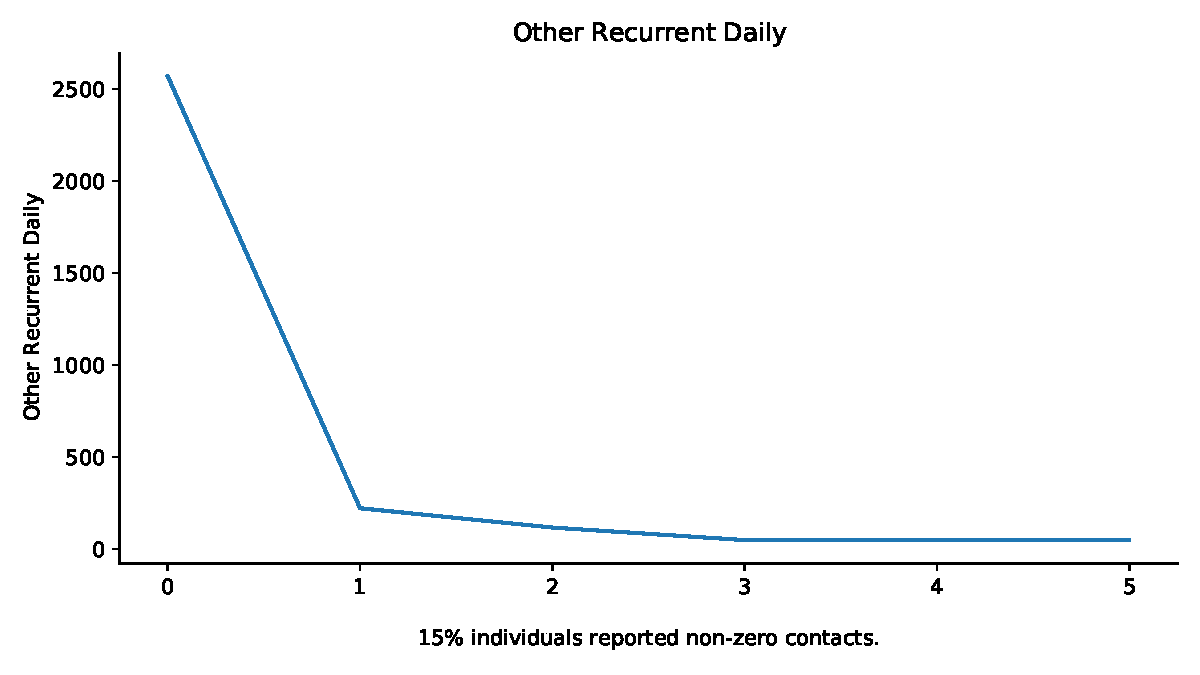
\includegraphics[width=\textwidth]{../figures/results/figures/data/distributions_of_the_number_of_contacts/other_recurrent_daily}
    \caption{Number of Daily Recurrent Other Contacts}
    \label{n_contacts_other_daily_recurrent}
    \floatfoot{\noindent Individuals are assigned to groups that are time constant and
    that meet daily. The share of individuals that attend in a way that has transmission
    potential is reduced by policies, seasonality and individual responses to events such
    as receiving a positive rapid test. Other contacts include all contacts that are not
    household members, school contacts or work contacts, for example leisure contacts or
    contacts during grocery shopping.}
\end{figure}


\begin{figure}
    \centering
    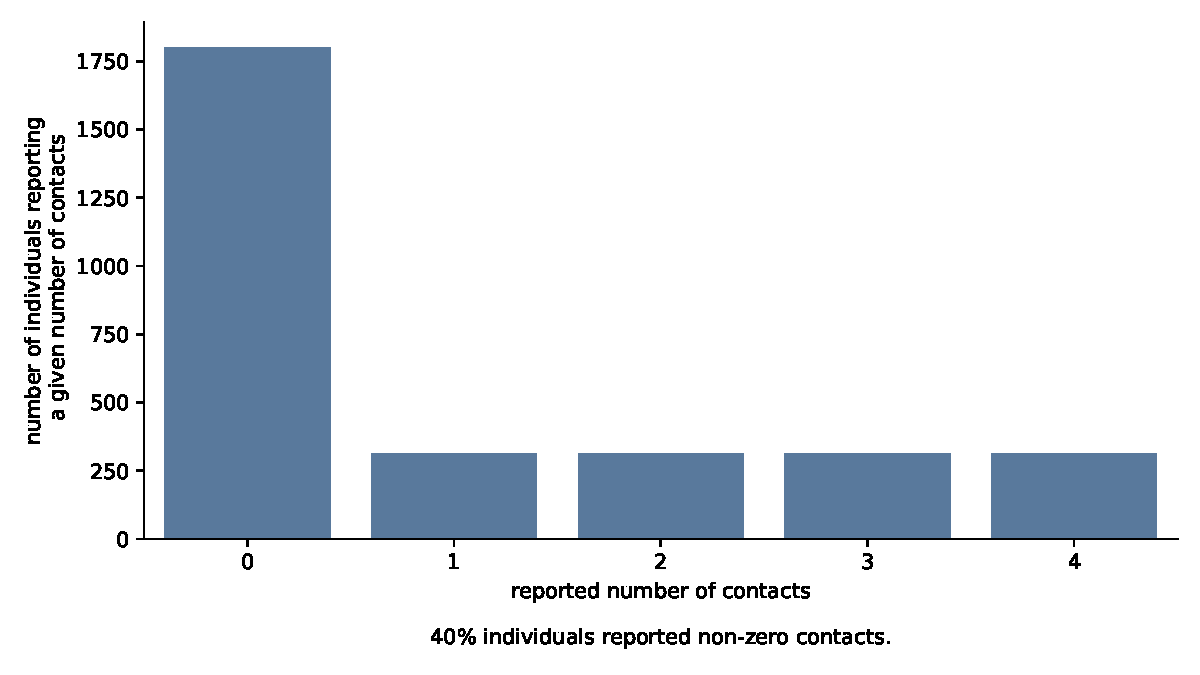
\includegraphics[width=\textwidth]{../figures/results/figures/data/distributions_of_the_number_of_contacts/other_recurrent_weekly}
    \caption{Number of Weekly Recurrent Other Contacts}
    \label{n_contacts_other_weekly_recurrent}
    \floatfoot{\noindent Individuals are assigned to up to four groups that are time
    constant and that meet weekly. The share of individuals that attend in a way that has
    transmission potential is reduced by policies, seasonality and individual responses
    to events such as receiving a positive rapid test. Other contacts include all
    contacts that are not household members, school contacts or work contacts, for
    example leisure contacts or contacts during grocery shopping.}
\end{figure}

% work contacts

\begin{figure}
    \centering
    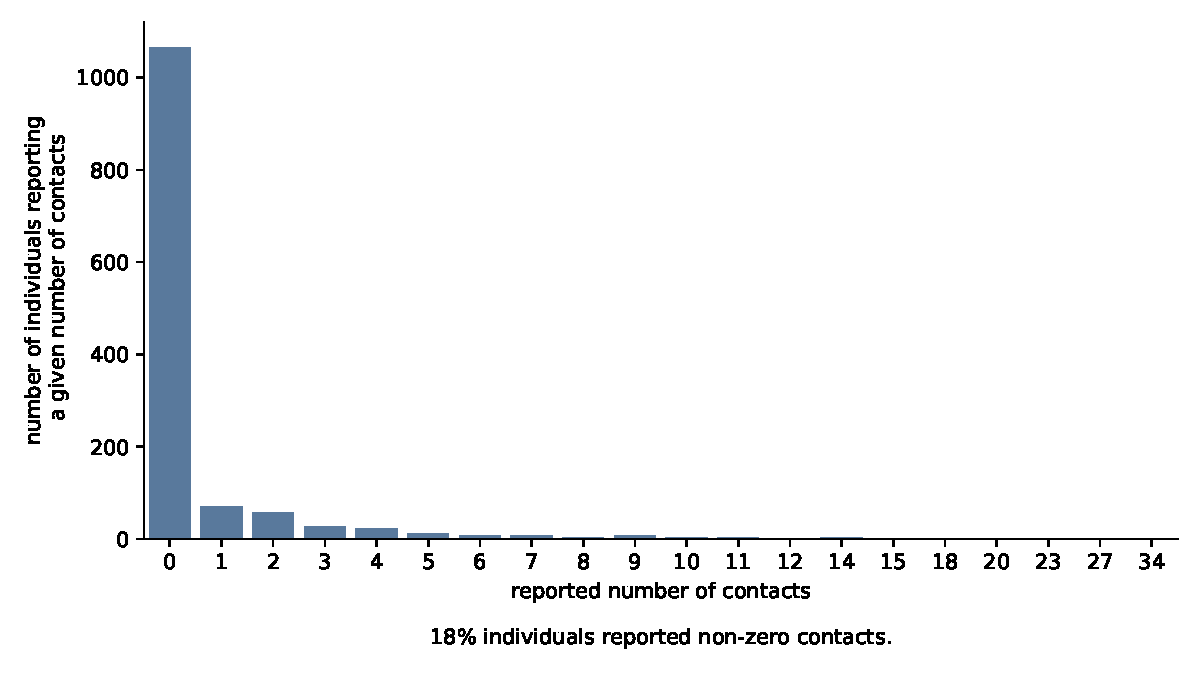
\includegraphics[width=\textwidth]{../figures/results/figures/data/distributions_of_the_number_of_contacts/work_non_recurrent}
    \caption{Number of Non Recurrent Work Contacts}
    \label{n_contacts_work_non_recurrent}
    \floatfoot{\noindent In the model it is sampled every day which of these numbers of
    contacts a working person is planned to have. Note that the contact diaries include
    such high values that super spreading events are well possible in our model. The
    planned number of contacts is reduced by policies, seasonality and individual
    responses to events such as receiving a positive rapid test to the number of actual
    contacts with transmission potential. Work contacts only take place between working
    individuals.}
\end{figure}


\begin{figure}
    \centering
    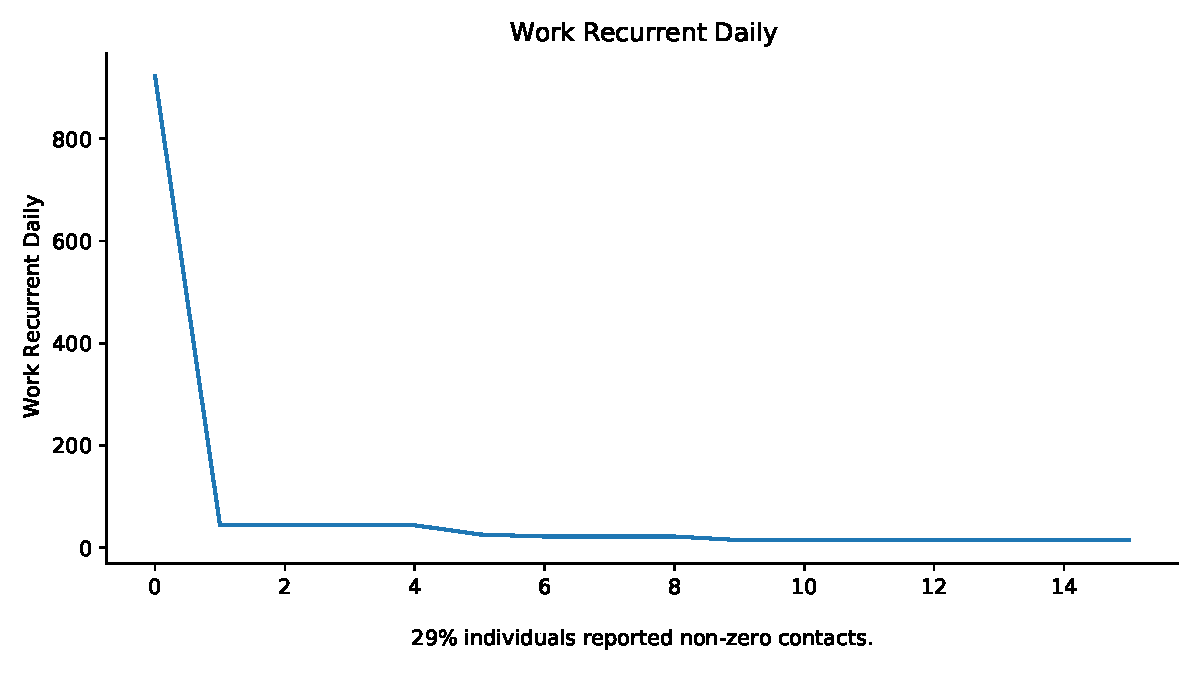
\includegraphics[width=\textwidth]{../figures/results/figures/data/distributions_of_the_number_of_contacts/work_recurrent_daily}
    \caption{Number of Daily Recurrent Work Contacts}
    \label{n_contacts_work_daily_recurrent}
    \floatfoot{\noindent Working individuals are assigned to groups that are time
    constant and that meet daily to match the given distribution of daily work contacts.
    You can think of these as for example colleagues with which one shares an office
    space. The share of individuals that attend in a way that has transmission potential
    is reduced by policies (such as a work from home mandate), seasonality and individual
    responses to events such as receiving a positive rapid test. Work contacts only take
    place between working individuals.}
\end{figure}


\begin{figure}
    \centering
    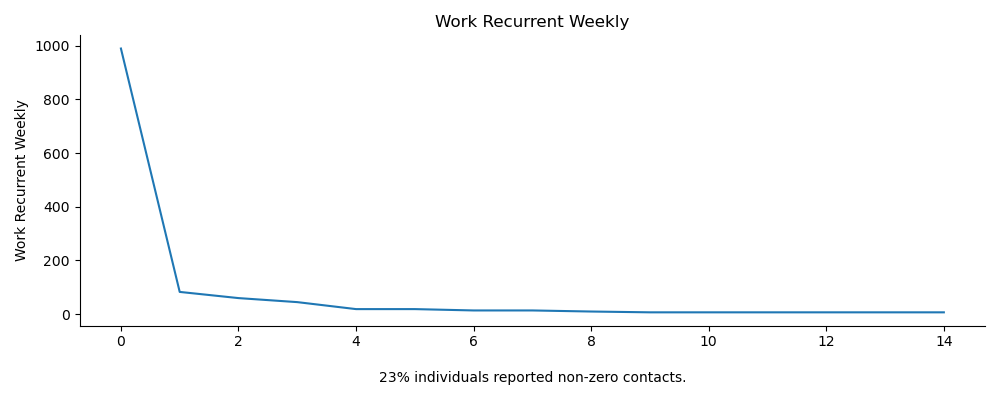
\includegraphics[width=\textwidth]{../figures/results/figures/data/distributions_of_the_number_of_contacts/work_recurrent_weekly}
    \caption{Number of Weekly Recurrent Work Contacts}
    \label{n_contacts_work_weekly_recurrent}
    \floatfoot{\noindent  Working individuals are assigned to up to 14 groups that are time
    constant and meet weekly. Groups are scheduled to meet on separate days of the work
    week. These contact models cover weekly team meetings etc. The share of individuals
    that attend in a way that has transmission potential is reduced by policies,
    seasonality and individual responses to events such as receiving a positive rapid
    test. Work contacts only take place between working individuals.}
\end{figure}


\FloatBarrier


\subsection{Contacts by age}
\label{subsec:contacts_by_age}

As mentioned in section \ref{sec:matching}, the probability that two individuals are
matched can depend on background characteristics. In particular, we allow this
probability to depend on age and county of residence. While we do not have good data on
geographical assortativity and just roughly calibrate it such that 80\% of contacts are
within the same county, we can calibrate the assortative mixing by age from the same
data we use to calibrate the number of contacts.\comment[id=HM]{Redo
\ref{fig:assortativity_other} /\ref{fig:assortativity_work} with total number of
contacts or better add a similar figure showing total number of contacts by age in all
networks}

\begin{figure}[ht]
    \centering
    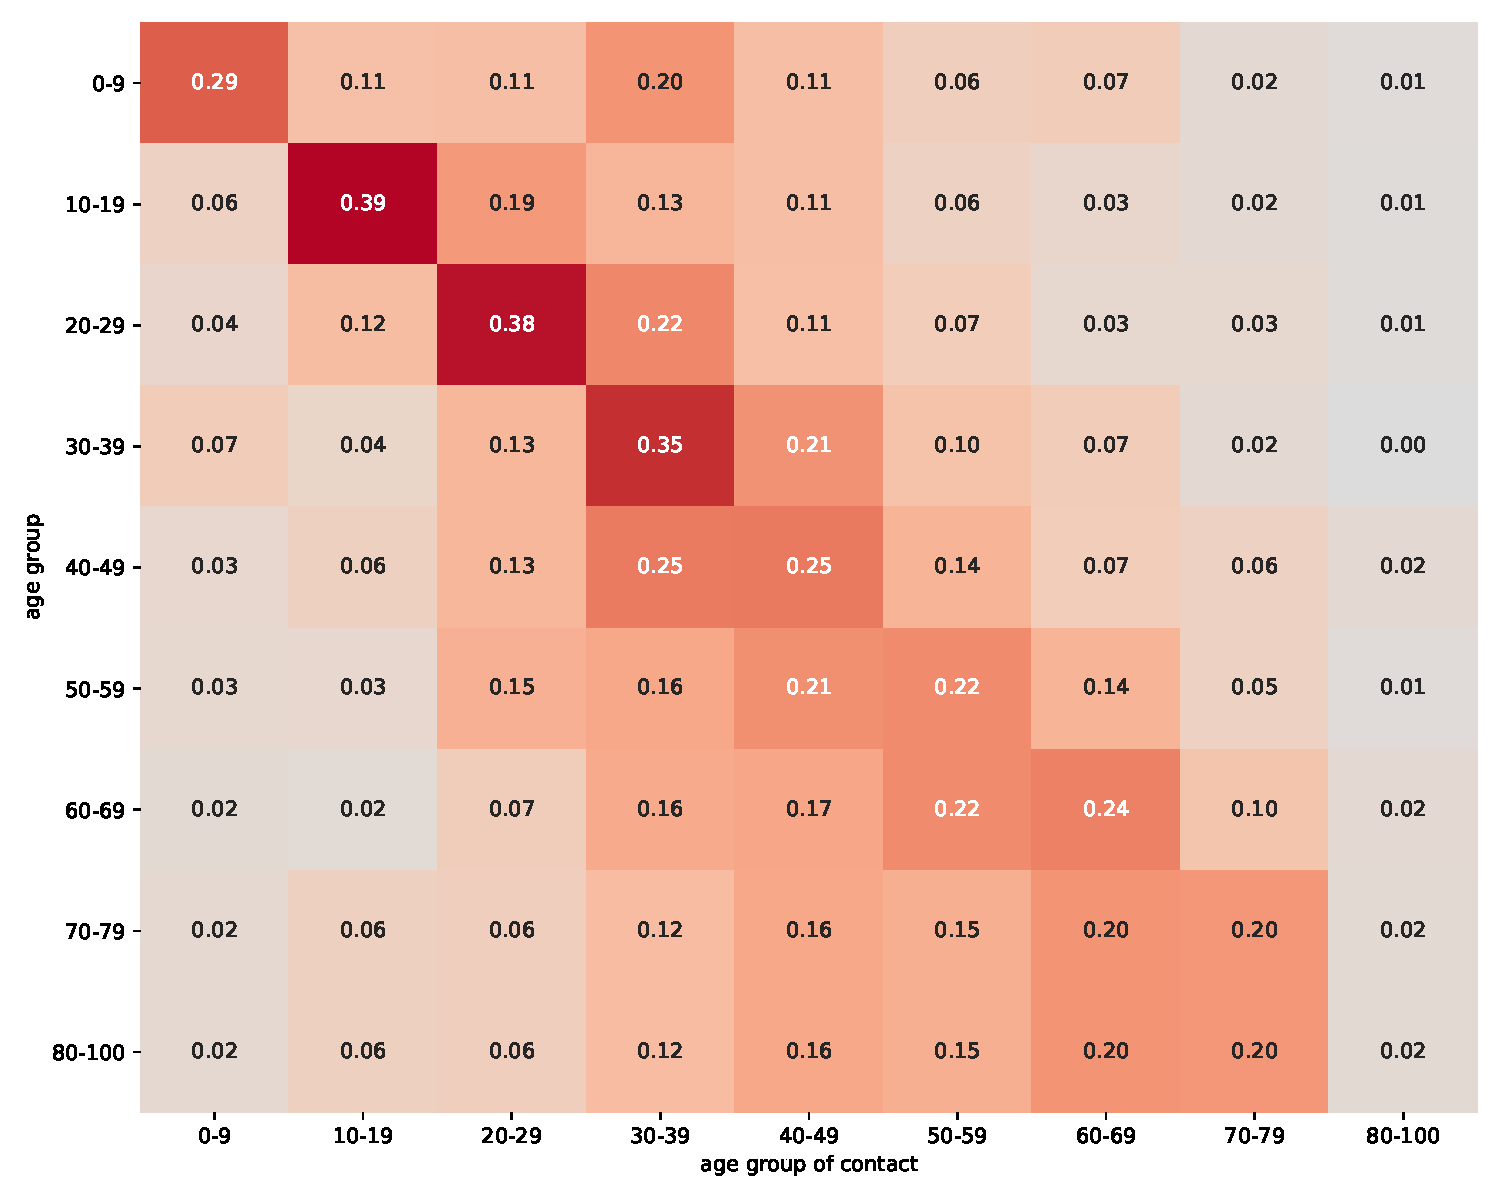
\includegraphics[width=0.9 \textwidth]{../figures/results/figures/data/assortativity_other_non_recurrent}
    \caption{Distribution of Non Recurrent Other Contacts by Age Group}
    \label{fig:assortativity_other}
    \floatfoot{\noindent The figure shows the distribution of non recurrent other contacts by age
        group. A row shows the share of contacts a certain age group has with all other
        age groups. Higher values are colored in darker red tones. The diagonal
        represents the share of contacts with individuals from the same age group.}
\end{figure}


Figure~\ref{fig:assortativity_other} shows that assortativity by age is especially strong
for children and younger adults. For older people, the pattern becomes more dispersed
around their own age group, but within-age-group contacts are still the most common
contacts.

\begin{figure}[ht]
    \centering
    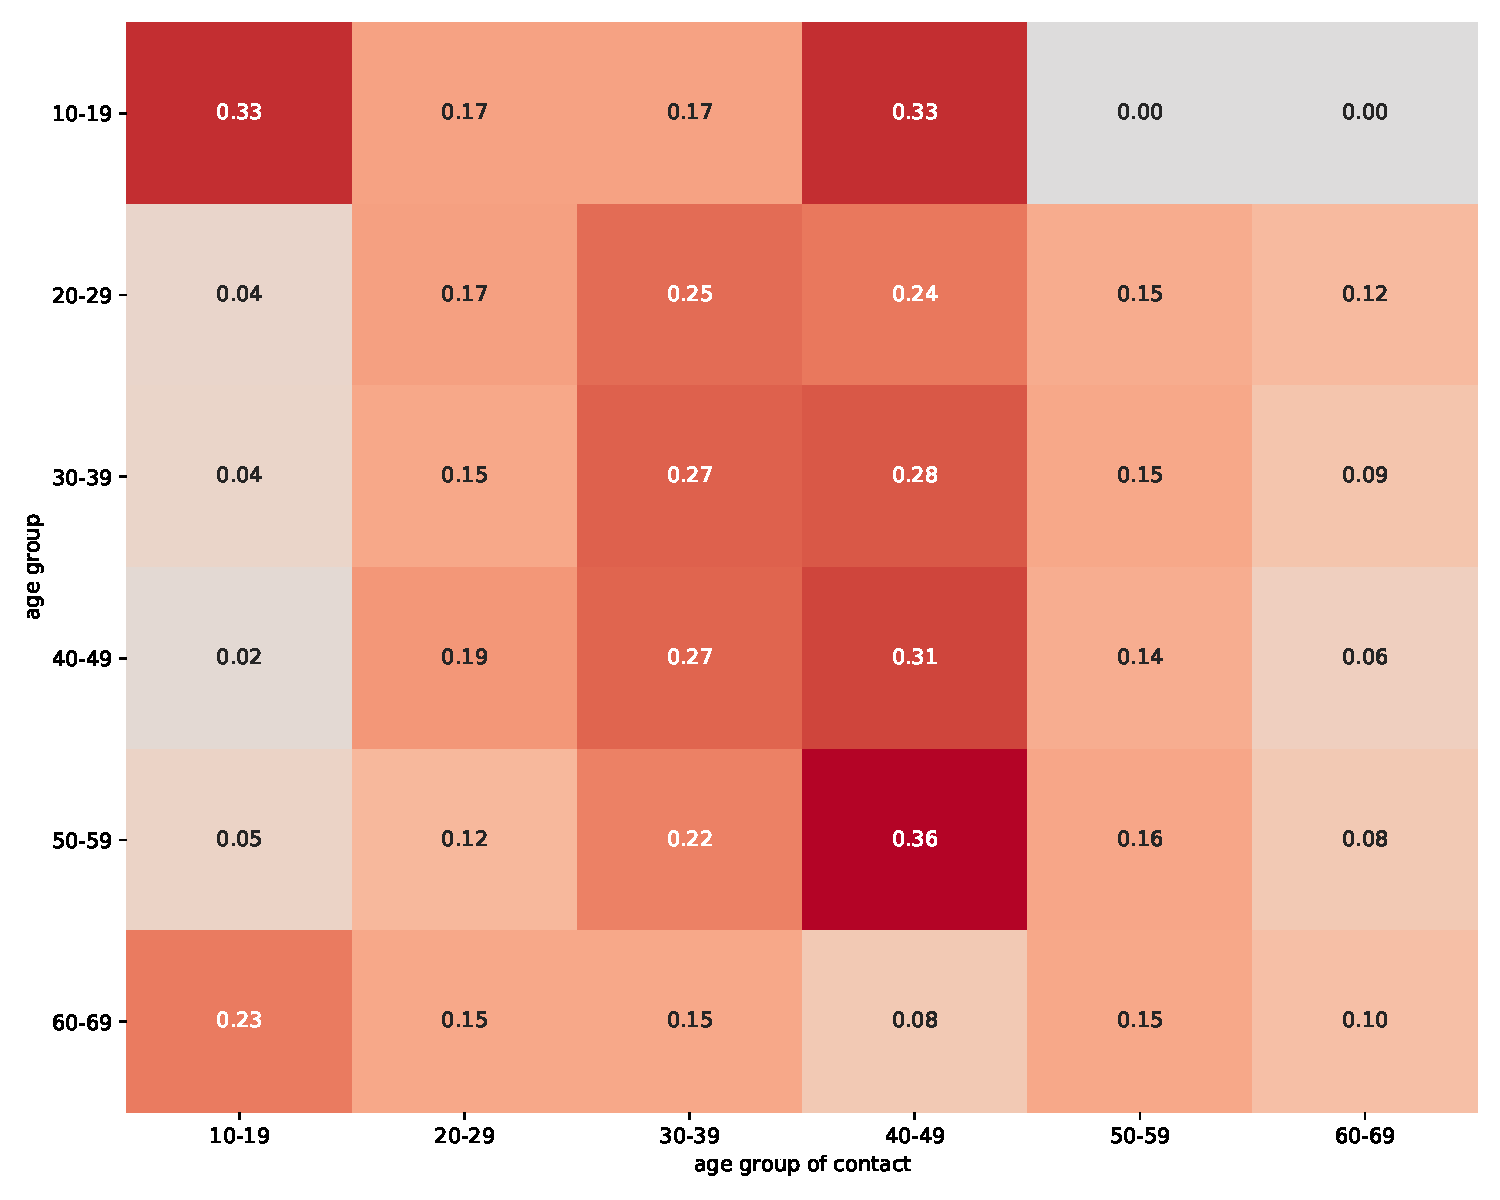
\includegraphics[width=0.9 \textwidth]{../figures/results/figures/data/assortativity_work_non_recurrent}
    \caption{Distribution of Random Work Contacts by Age Group}
    \label{fig:assortativity_work}
    \floatfoot{\noindent The figure shows the distribution of non recurrent work contacts by age
        group. A row shows the share of contacts a certain age group has with all other
        age groups. Higher values are colored in darker red tones. The diagonal
        represents the share of contacts with individuals from the same age group. We
        only show age groups that have a significant fraction of working individuals.}
\end{figure}

Figure~\ref{fig:assortativity_work} shows that assortativity by age is also important
among work contacts.

Our other two types of contacts, households and schools, get their assortativity by
construction. Schools are groups where the same children of the mostly same age group and
county meet with teachers every day. Household composition follows directly from the
German microcensus data we use to construct our synthetic population.\comment[id=HM]{So
no work in here? How about school? Can we add a column with marginals and another one
with work / (school?), too?}\comment[id=K]{I hope adding work and writing about school and
households addresses all questions. I think marginals would be confusing because they may not add up to one given that age groups have different group sizes.}

\FloatBarrier


\subsection{Infection Probabilities}
\label{sec:estimation}

To calibrate infection probabilities outside of the model, it would be important to know
the exact duration and distance of each contact type as well as viral loads. Since this
is not available in any data set, we estimate those parameters inside the model with the
method of simulated moments \citep{McFadden1989} by minimizing the distance between
simulated and observed infection rates. Since our model includes a lot of randomness, we
average simulated infection rates over several model runs.

Currently, we use data for Germany from October 2020 until June 2021. We do not use
earlier periods for three reasons. Firstly, in the beginning PCR tests were highly
limited and therefore it would be difficult to find good initial conditions for our
simulations. In addition during the summer the case numbers were extremely low. This
could lead to the epidemic going extinct in our simulation. Additionally, our model does
not include international travel or other imports of cases. These would be important but
difficult to model during the summer months.

To avoid over-fitting and simplify the numerical optimization problem, we only allow for
five different probabilities: 1) for contacts in schools 2) contacts in preschools and
nurseries. 3) for work contacts. 4) for households. 5) for other contacts.

The infection probabilities estimated from our model are as follows: For household
contacts (each individual meets all his or her household members every day) the infection
probability is 10\%, for school contacts (all students and teachers meet all other
students and teachers that attend school that day and there are three classes taking
place each day) the probability of infection is 1.2\%, for preschools and nurseries that
infection probability is 0.5\%. Work contacts carry a risk of 14.5\% and other activities
(including leisure activities such as meeting friends) carry the highest risk with
15.875\%.

\subsection{Policies}

\FloatBarrier

In our empirical application we distinguish four groups of contact types: households,
education, work and other contacts. For households we assume that the individuals'
contacts in their households do not change over our estimation period. For nurseries,
preschools and schools we implement vacations as announced by the German federal states
as well as school closures, emergency care and A / B schooling where only one half of
students attends every other week or day. For the moment we ignore that lack of childcare
leads working parents to stay home.
%
% Schließung von Kindertagesstätten und Schulen: 37,4 Millionen ausgefallene Arbeitstage
% http://www.iab-forum.de/schul-und-kitaschliessungen-krankheit-quarantaene-die-coronabedingten-arbeitsausfaelle-der-erwerbstaetigen-steigen-auf-592-millionen-arbeitstage/
%
%
% https://www.sueddeutsche.de/politik/schulschliessung-lockdown-bildung-1.5190377: In
% allen Ländern geht trotz des Lockdowns ein erheblicher Anteil der Schülerinnen und
% Schüler in die Schule.
% https://gfx.sueddeutsche.de/apps/e525337/www/_image_desktopw1840q70-1e2e2bf78b7d4430
% 18% der Grundschüler in Notbetreuung in BW
%
For our work models\footnote{We distinguish non-recurrent work contacts, daily work
contacts and weekly work contacts.} we use the reductions in work mobility reported in
the Google Mobility Data \citep{Google2021} to calibrate our work policies. Reductions in
work contacts are not random but governed through a work contact priority where the
policy changes the threshold below which workers stay home. Figure
\ref{fig:work_multiplier} shows the share of workers that go to work in our model over
time.

\begin{figure}[ht]
    \centering
    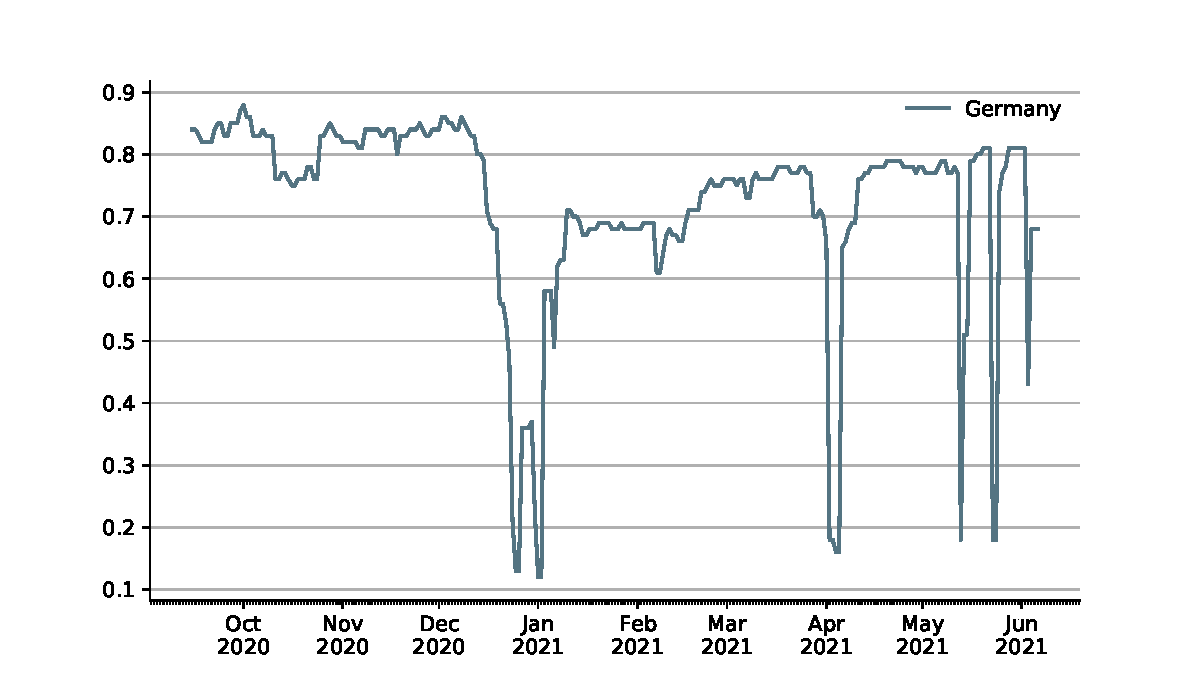
\includegraphics[width=\textwidth]{../figures/results/figures/data/work_multiplier_since_sep}
    \caption{Share of Workers with Work Contacts}
    \label{fig:work_multiplier}
    \floatfoot{\noindent The figure shows the work mobility as reported by \cite{Google2021}. We
        take this as a proxy of the share of workers who are not in home office, i.e. who
        still have physical work contacts. The figure interpolates over weekends as we
        handle weekend effects through information on work on weekends in the German
        census data we use. The figure shows the share aggregated over Germany as a
        whole. To capture the effect that local policies, school vacations and public
        policies have on work contacts we use the data by German state to determine which
        workers go to work depending on the state they live in.}
\end{figure}


For the last group of contacts which cover things like leisure activities, grocery
shopping etc. we have no reliable data by how much policies reduce them. In addition,
they are likely to be affected by social and psychological factors such as pandemic
fatigue and vacations. Because of this we estimate them like the infection probabilities
to fit the time series data. We use very few change points and tie them to particular
events such as policy announcements or particular holidays.

\FloatBarrier

\subsection{Rapid Test Demand}


\begin{figure}
    \centering
    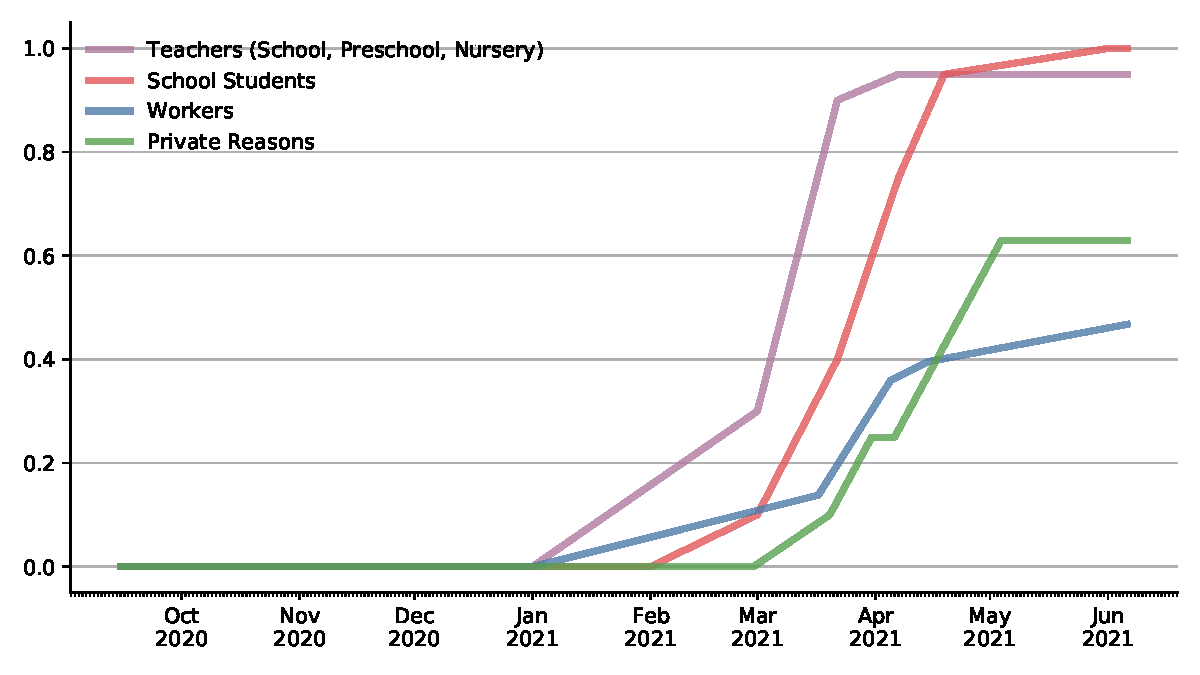
\includegraphics[width=\textwidth]{../figures/results/figures/data/testing/rapid_test_demand_shares}
    \caption{\textbf{Share of Individuals that do a Rapid Test.}}
    \floatfoot{\noindent \textcolor{red}{J: Talk about the interpretation of each line.}}
    \label{fig:rapid_test_demand}
\end{figure}

In our model, there are five reasons why rapid tests are done:
\begin{enumerate}
    \item someone plans to have work contacts
    \item someone is an employees of an educational facility or school pupil
    \item someone lives in a household where someone has tested positive or developed
          symptoms
    \item someone has developed symptoms but has not received a PCR test
    \item someone plans to participate in a weekly non-work meeting
\end{enumerate}

% work rapid tests

For work contacts, we know from the COSMO study (\cite{Betsch2021}, 20th/21st of April)
that 60\% of workers who receive a test offer by their employer regularly use it. We
assume this to be time constant.

In addition, there are some surveys that allow us to trace the expansion of employers
who offer tests to their employees. Mid march, 20\% of employers offered tests to their
employees \citep{DIHK2021}. In the second half of March, 23\% of employees reported
being offered weekly rapid tests by their employer \citep{Ahlers2021}. This share
increased to 60\% until the first days of April \cite{ZDF2021}. Until mid April 70\% of
workers were expected to receive a weekly test offer \citep{AerzteZeitung2021}. However,
according to surveys conducted in mid April \citep{Betsch2021}, less than two thirds of
individuals with work contacts receive a test offer. Starting on April 19th employers
were required by law to provide two weekly tests to their employees
\citep{Bundesanzeiger2021}. We assume that compliance is incomplete and only 80\% of
employers actually offer tests.\comment[id=HM]{Can we use the IZA/BMAS survey? Not sur
about citing evening news in scientific papers.}

% educ rapid tests

\comment[id=J]{Sources still missing below this}

We assume that employees in educational facilities start getting tested in 2021 and that
by March 1st 30\% of them are tested weekly. The share increases to 90\% for the week
before Easter. At that time both Bavaria and Baden-Württemberg were offering tests to
teachers and North-Rhine Westphalia and Lower Saxony were already testing students and
tests for students and teachers were already mandatory in Saxony. After Easter we assume
that 95\% of teachers get tested twice per week.

Tests for students started later so we assume that they only start in February and only
10\% of students get tested by March 1st. Relying on the same sources as above we
approximate that by the week before Easter this share had increased to 40\%.

After Easter we assume the share of students receiving twice weekly tests to based on
tests already being mandatory in North-Rhine Westphalia and Bavaria while still being
voluntary in Baden-Württemberg. There tests become mandatory on April 19th.


% household member rapid tests



% own symptom rapid test demand



% private meeting test demand



\comment[id=J]{Add a section on how we calibrate rapid test demand; Mainly describe the
datapoints we have and say that we usually interpolate linearly in between data points.
(Only exception to that is private rapid test demand, which we fit to data)}


\begin{figure}[ht]
    \centering
    \caption{Share of Individuals With Rapid Tests}
    \label{fig:share_ever_rapid_test}
    \begin{subfigure}{.55\textwidth}
        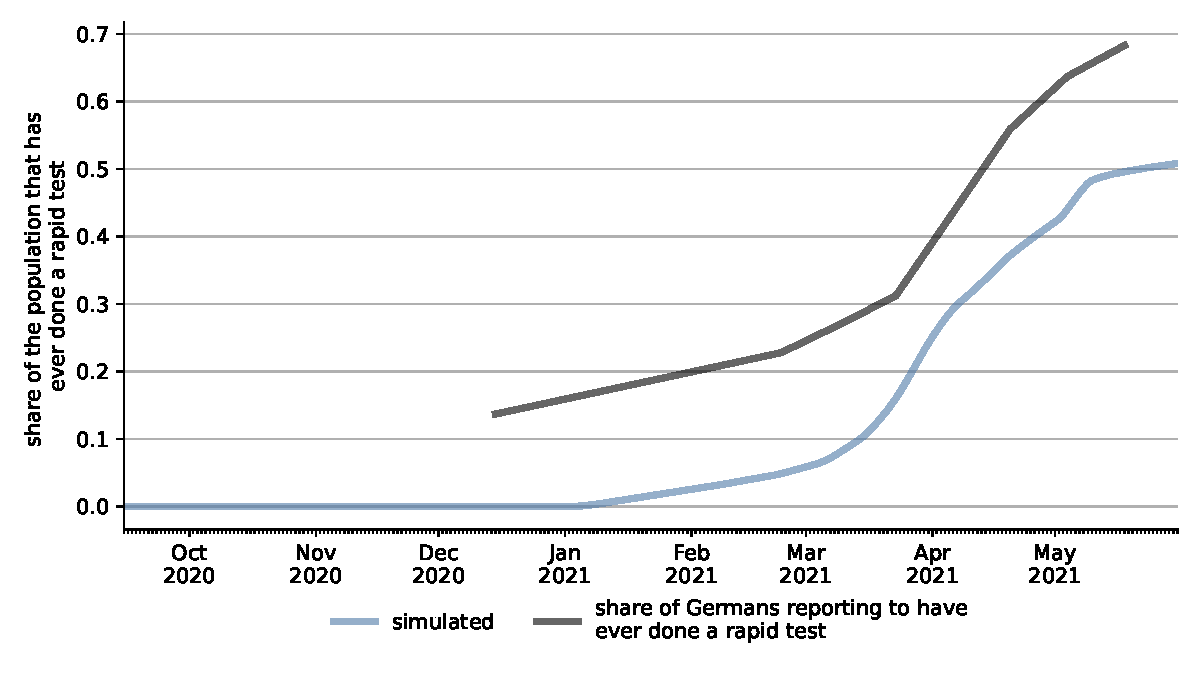
\includegraphics[width=0.9 \textwidth]{../figures/results/figures/scenario_comparisons/combined_fit/full_share_ever_rapid_test}
    \end{subfigure}%
    \begin{subfigure}{.55\textwidth}
        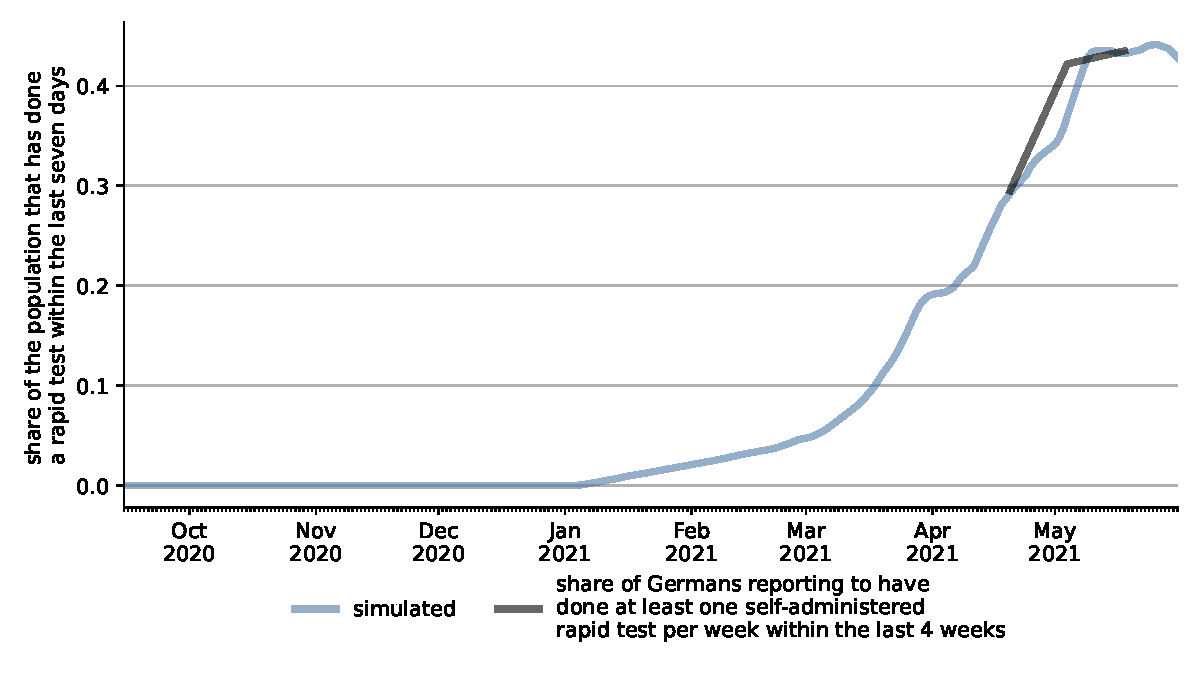
\includegraphics[width=0.9 \textwidth]{../figures/results/figures/scenario_comparisons/combined_fit/full_share_rapid_test_in_last_week}
        %   \caption{Share of Individuals Having Done a Rapid Test in the Last Week}
    \end{subfigure}
    \label{fig:share_rapid_test_last_week}
    \floatfoot{\noindent The figure compares the share of individuals who have ever done a rapid
        test or done a rapid test within the last week in our simulations to the shares
        reported in the
        \href{https://projekte.uni-erfurt.de/cosmo2020/web/topic/wissen-verhalten/80-schnelltests/}{COVID-19
            Snapshot Monitoring survey}. The left panel compares the share of individuals
        who have ever done a rapid test. The right panel compares the share of
        individuals who have done a rapid test within the last seven days in our
        simulation compared to the share reporting to have done at least weekly rapid
        tests in the last four weeks in the COSMO survey. Overall our calibration of
        rapid tests are slightly conservative. The overall share is below that in the
        study. We fit the share of weekly tests quite exactly. However, the study only
        covers adults while our share also includes children who are tested very
        regularly when attending school.}
\end{figure}


    \FloatBarrier

    \section{Detailed Model Description}
\label{sec:model}

\subsection{Literature Review}
\label{sec:literature_review}

We build on two strands of literature: Recent extensions of the epidemiological SEIR
model and agent-based simulation models.

The traditional SEIR model is not fine-grained enough to model nuanced policies. This
has motivated a large number of researchers to extend the standard model to allow for
more heterogeneity and flexibility. Examples are \citet{Grimm2020},
\citet{Donsimoni2020} and \citet{Acemoglu2020} who develop multi group SEIR models to
analyze the effects of targeted lockdowns and \citet{Berger2020} who extend the SEIR
model to analyze testing and conditional quarantines. For a more comprehensive review
see \citet{Avery2020}. Others have used the results of a standard SEIR model as input
for economic models that estimate the cost of policies (e.g. \citet{Dorn2020}).

While the popularity of the SEIR model is mainly due to its simplicity, the extensions
are quite complex. It is unlikely that there will be a SEIR model that combines all
proposed extensions. Moreover, the extensions do not address other key issues: The main
parameter of the SEIR model, the basic reproduction number ($R_0$), is not
policy-invariant. It is a composite of the number of contacts each person has and the
infection probability of the contacts. In fact, policy simulations are done by setting
$R_0$ to a different value but it is hard to translate a real policy into the value of
$R_0$ it will induce. In other words, SEIR models are not suited for evaluating the
effect of policies which have never been experienced before.

Another commonly used model class in epidemiology are agent-based simulation models. In
these models individuals are simulated as moving particles. Infections take place when
two particles come closer than a certain contact radius (e.g. \citet{Silva2020} and
\citet{Cuevas2020}). While the simulation approach makes it easy to incorporate
heterogeneity in disease progression, it is hard to incorporate heterogeneity in meeting
patterns. Moreover, policies are modeled as changes in the contact radius or momentum
equation of the particles. The translation from real policies to corresponding model
parameters is a hard task.

\citet{Hinch2020} is a recent extension of the prototypical agent-based simulation model
that replaces moving particles by contact networks for households, work and random
contacts. This model is similar in spirit to ours but focuses on contact tracing rather
than social distancing policies.

The above assessment of epidemiological models is not meant as a critique. We are aware
that these models were not designed to predict the effect of fine-grained social
distancing policies in real time and are very well suited to their purpose. We invite
epidemiologists to provide feedback and collaborate to improve our model.


\subsection{Summary}
\label{sub:model_summary}

To alleviate these problems we propose a different model structure. Our model inherits many features from agent-based simulation models but replaces the contacts between moving particles by contacts between individuals who work, go to school, live in a household and enjoy leisure activities. The structure of the model is depicted in Figure~\ref{fig:model_graph}.

\begin{figure}[!ht]
    \centering
    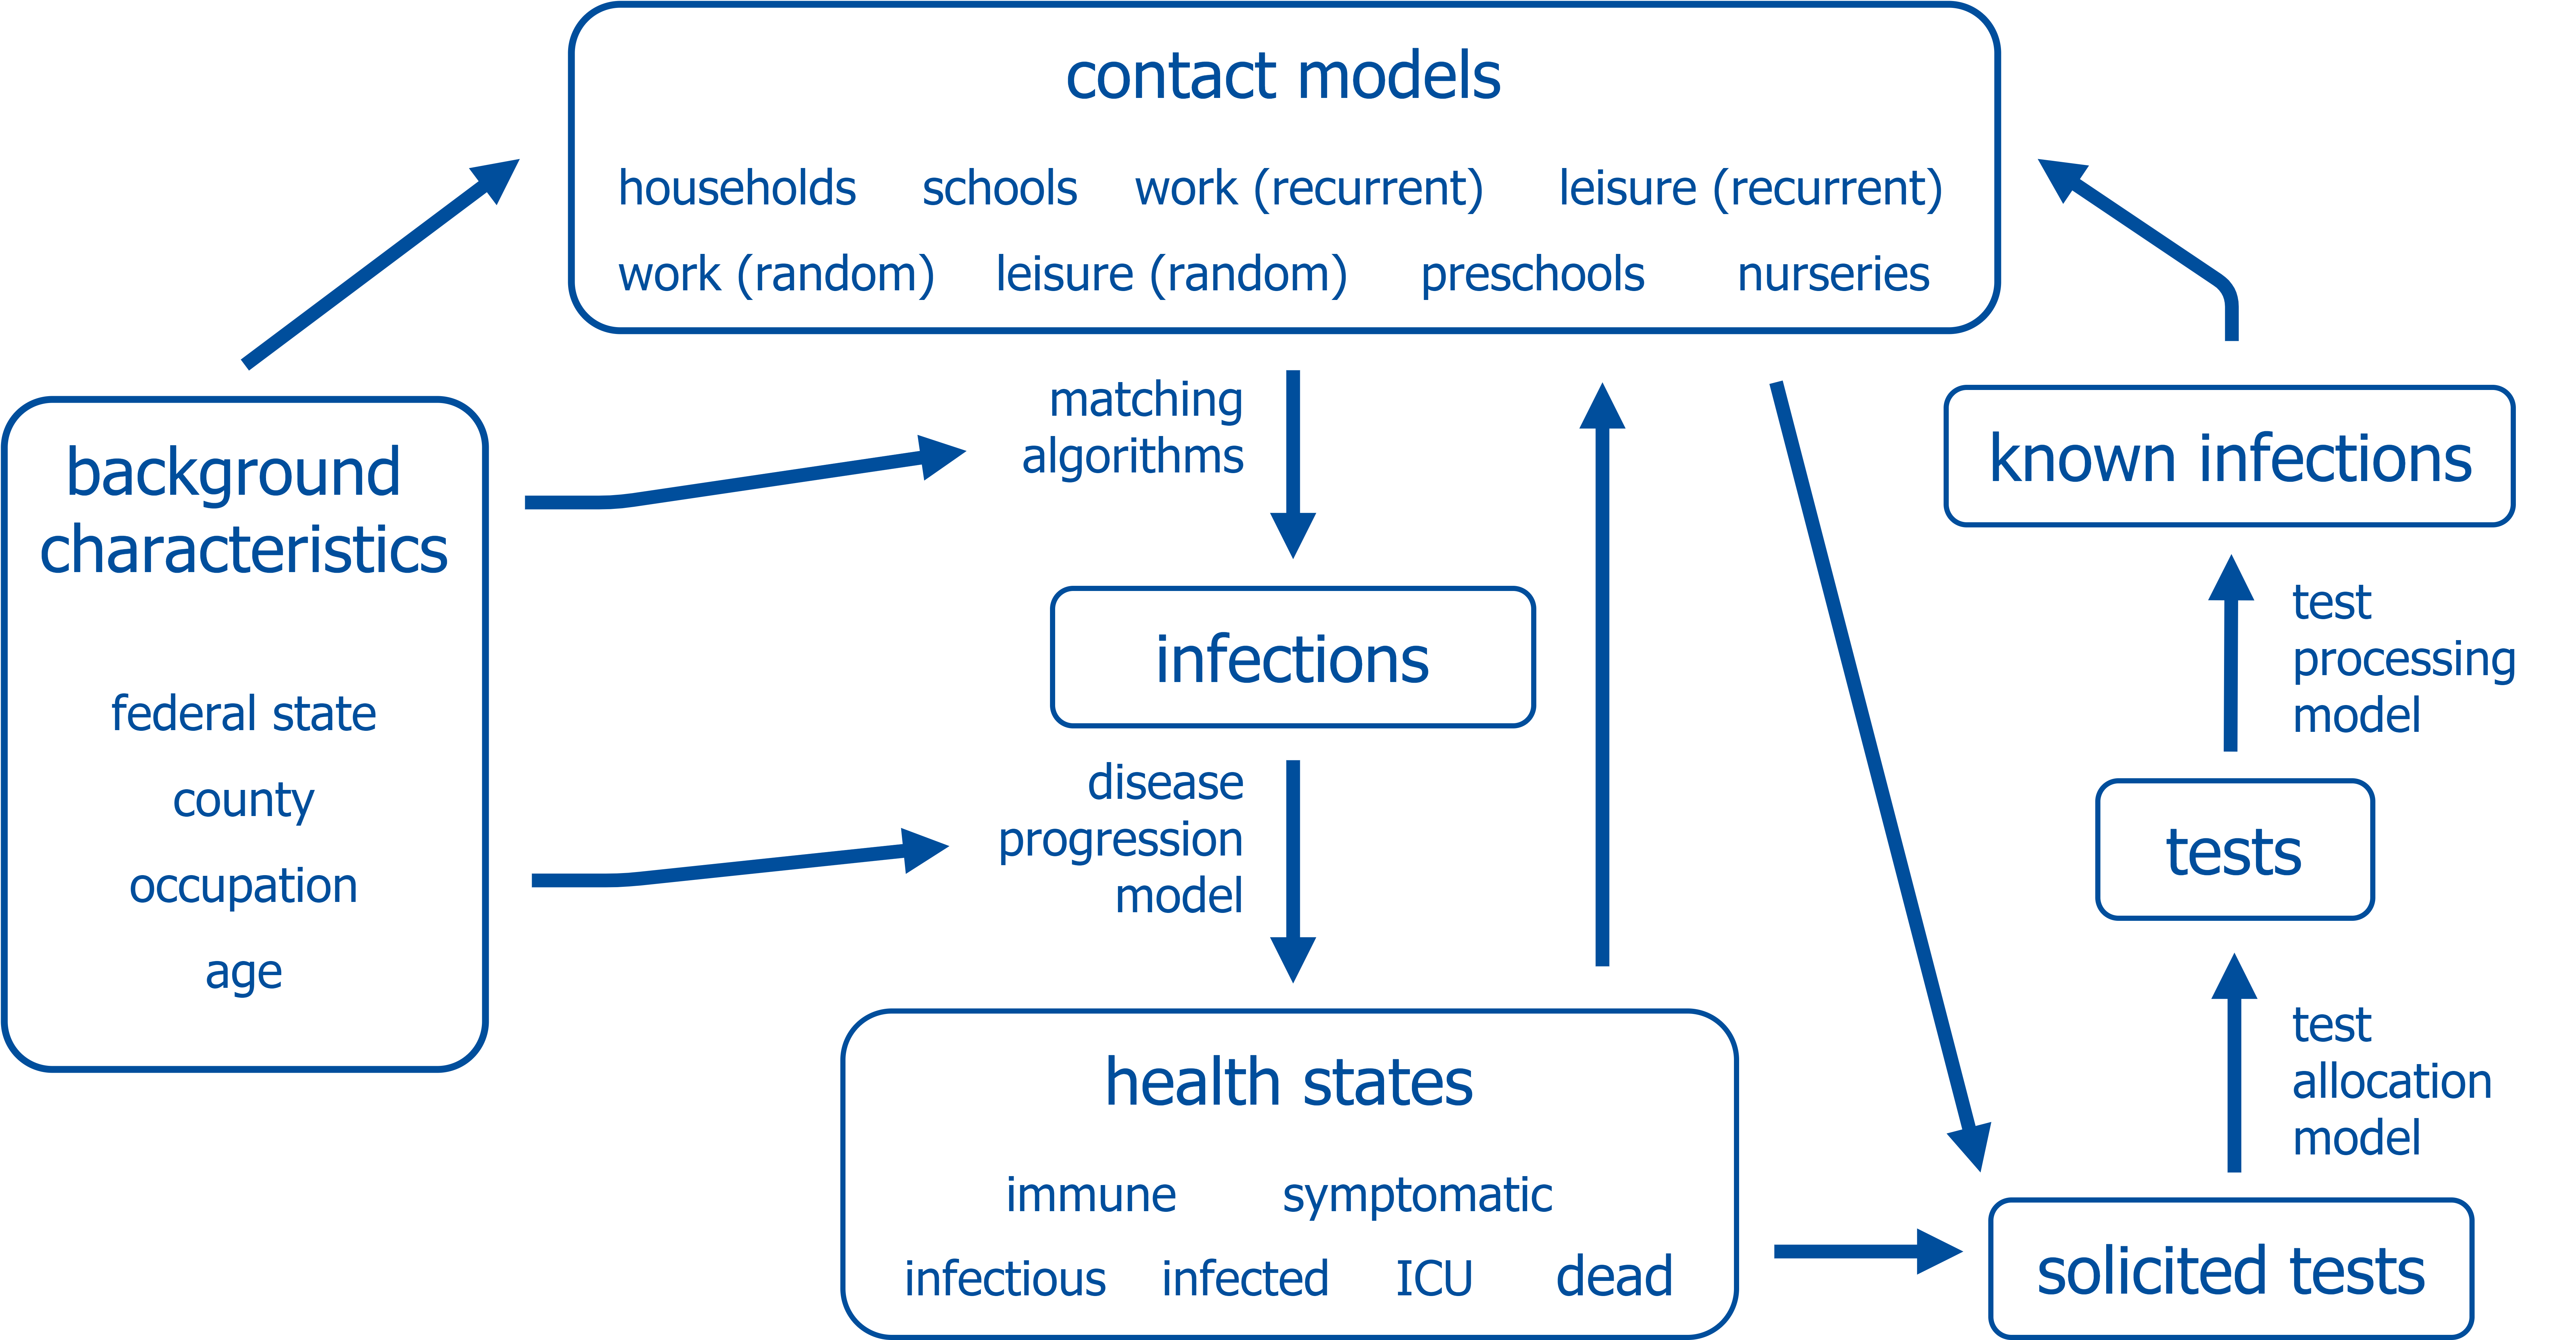
\includegraphics[width=0.7\textwidth]{../figures/model_detailed.png}
    \caption{Simplified graph of the model}
    \label{fig:model_graph}
\end{figure}

The background characteristics include age, county and occupation of each simulated individual. Contact models are functions that map individual characteristics into a predicted number of contacts. Currently we distinguish between eight types of contact models which are all listed in Figure~\ref{fig:model_graph}: households, recurrent and random work contacts, recurrent and random leisure contacts, and nursery, preschool, and school contacts.

The predicted number of contacts is translated into infections by a matching algorithm. There are different matching algorithms for recurrent contacts (e.g. classmates, family members) and non-recurrent contacts (e.g. clients, contacts in supermarkets). The infection probability can differ for each contact type. All types of contacts can be assortative with respect to geographic and demographic characteristics.

Once a person is infected, the disease progresses in a fairly standard way which is also depicted in Figure~\ref{fig:course_of_disease}. Asymptomatic cases and cases with mild symptoms are infectious for some time and recover eventually. Cases with severe symptoms additionally require hospitalization and lead to either recovery or death.

There are two possible ways to enable testing for Covid-19 in the model. The first way allows to specify the ratio of known to unknown infections for each day. A random sample of all newly infected individuals will then receive a test result in the following days. The second approach consists of three steps. First, individuals demand a test because they, e.g., experience symptoms. Secondly, tests are allocated to individuals while respecting governmental access restrictions to test. Thirdly, depending of the capacities of laboratories, tests are processed for some time until the individual receives her test result.

In addition, people who have symptoms, received a positive test, or had a risk contact can reduce their number of contacts across all contact types endogenously.

The model makes it very simple to translate policies into model quantities. For example, school closures imply the complete suspension of school contacts. A strict lockdown implies shutting down work contacts of all people who are not employed in a systemically relevant sector. It is also possible to have more sophisticated policies that condition the number of contacts on observable characteristics, risk contacts or health states.

Another key advantage of the model is that the number of contacts an individual has of each contact type can be calibrated from publicly available data \citep{Mossong2008}. This in turn allows us to estimate policy-invariant infection probabilities from time series of infection and death rates using the method of simulated moments \citep{McFadden1989}. Since the infection probabilities are time-invariant, data collected since the beginning of the pandemic can be used for estimation. Moreover, since we can model the testing strategies that were in place at each point in time, we can correct the estimates for the fact that not all infections are observed.

Last but not least, performing simulations whose starting point is set amidst the pandemic requires special adjustments to arrive at a realistic distribution of courses of diseases. We solve the initial conditions problem by matching reported infections to individuals in our data while also correcting for reporting lag and undetected cases.

In the following sections we describe each of the model components in more detail.


\subsection{Modeling Numbers of Contacts}
\label{sec:number_of_contacts}

Consider a hypothetical population of 1,000 individuals in which 50 were infected with a
novel infectious disease. From this alone, it is impossible to say whether only
those 50 people had contact with an infectious person and the disease has an infection
probability of 1 per contact or whether everyone met an infectious person but the
disease has an infection probability of only 5 percent per contact. SEIR models do not
distinguish contact frequency from the infectiousness of each contact and
combine the two in one parameter that is not invariant to social distancing policies.

To model social distancing policies, we need to disentangle the effects of the number of
contacts of each individual and the effect of policy-invariant infection probabilities
specific to each contact type. Since not all contacts are equally infectious, we
distinguish different contact types.

The number and type of contacts in our model can be easily extended. Each type of
contacts is described by a function that maps individual characteristics, health states
and the date into a number of planned contacts for each individual. This allows to model
a wide range of contact types.

In our empirical application we distinguish the following  contact types that
are depicted in Figure~\ref{fig:model_contacts_infections} and can be further grouped
in the categories household, work, education and others.

types of contacts:

\begin{itemize}
    \item Households: Each household member meets all other household members every day.
    % Household sizes and structures are calibrated to be representative for Germany.


    \item Recurrent work contacts, capturing contacts with coworkers, repeating
          clients and superiors. Some of these recurrent contacts take place on
          every workday, others just once per week.

    \item Random work contacts: Working adults have contacts with randomly drawn other
          people, which are assortative in geographical location and age.


    \item Schools: Each student meets all of his classmates every day. Class sizes are
    calibrated to be representative for Germany and students have the same age. Schools
    are closed on weekends and during vacations, which vary by states. School classes
    also meet six teachers everyday and some of the teachers meet each other.

    \item Preschools: Children who are at least three years old and younger than six may
    attend preschool. Each group of nine children interacts with the same two adults
    every day. The children in each group are of the same age. The remaining mechanics
    are similar to schools.

    \item Nurseries: Children younger than three years may attend a nursery and interact
    with one adult. The age of the children varies within groups. The remaining
    mechanics are similar to schools.

    \item Random other contacts: Contacts with randomly drawn other
    people, which are assortative with respect to geographic location and and age group.
    This contact type reflects contacts during leisure activities, grocery shopping,
    medical appointments, etc..

    \item Recurrent other contacts representing contacts with friends neighbors or
        family members who do not live in the same household. Some of these contacts
        happen daily, others only once per week.


\end{itemize}

The number of random and recurrent contacts at the workplace, during leisure activities
and at home is calibrated with data provided by \citet{Mossong2008}. For details see
Section~\ref{subsec:data_number_of_contacts}. In particular, we sample the number of
contacts or group sizes from empirical distributions that sometimes depend on age. It
would also be possible to use economic or other behavioral models to predict the number
of contacts.

% Theoretically, each contact type can have its own infection probability. However, to
% reduce the number of free parameters and thus avoid a potential over-fitting we only
% estimate different infection probabilities for the areas work, school, preschool and
% nurseries, households and other contacts.


\subsection{Reducing Numbers of Contacts via NPIs}
\label{sec:policies}

Our model makes it very easy to model a wide range of NPIs, either in isolation or
simultaneously. This is important for two reasons: Firstly, it allows to predict and
quantify the effect of novel NPIs. Secondly, it allows to model the actually implemented
policy environment in great detail, which is necessary to use use the full time series
of infections and fatality rates to estimate the model parameters.\footnote{
See \citet{Avery2020} for an explanation why it can be harmful to use too long time
series to estimate simple SEIR type models.}


Instead of thinking of policies as completely replacing how many contacts people have,
it is often more helpful to think of them as adjusting the pre-pandemic number of
contacts. Therefore, we implement policies as a step that happens after the number of contacts is
calculated but before individuals are matched.

On an abstract level, a policy is a functions that modifies the number of contacts of
one contact type. This function can be random or deterministic. For example, school
closures simply set all school contacts to zero. A work from home mandate leads to a
share of workers staying home every day whereas those who cannot work from home are
unaffected. Hygiene measures at work randomly reduce the number of infectious contacts
for all workers who still go to work.

Policies can also interact. For example, school vacations are temporally reducing school
contacts to zero while at the same time increasing other contacts to account for
increased leisure activities and family visits during this time. This is important to
reproduce the finding that school vacations do not reduce infection numbers even though
schools lead to infections when open \citep{Isphording2021}.

The most complex policies are typically found in the education sector. Since the
beginning of 2021 schools have switched back and fourth between full closures,
split class approaches with alternating schedules for some or all age groups and
reopening while maintaining hygiene measures. On top of that there are different
policies for allowing young students whose parents work full time to attend school
even on days where they normally would not. For details on how we calibrate these
policies see Section~\ref{subsec:policies}.

Importantly, policies can depend on the health states of participating individuals.
This allows to quarantine entire school classes if one student tested positive or
to implement official or private contact tracing.

For some policies the exact effect on each contact type is not easy to determine. If
this refers to a policy has been active during the estimation period, it is possible to
estimate such parameters by fitting the model to time series data of infection rates.
This is only possible if the policy was not active during the whole estimation period
and thus the infection probabilities can be identified separately. We do this to account
for hygiene measures at school and in the workplace that have been in effect since
November 2020.

Not all things that reduce contacts compared to the pre-pandemic level are driven
by NPIs. Therefore, we also model endogenous contact reductions that can depend on
the health state of individuals, known risk contacts or the local incidence of
infections. Examples are strong contact reductions for symptomatic individuals or those
who have a positive PCR or rapid tests or contact reductions when a houshold member
tested positive. The extent to which contacts are reduced can be calibrated from
surveys. For an application of our model showcasing private contact tracing in the
context of the Christmas holidays see \cite{Gabler2020}.








\subsection{Endogenous Contact Reductions}
\label{sec:endogenous_contact_reductions}

Policies are not the only way in which the number of contacts are reduced compared to
the pre-pandemic level. It is important to model those other channels. Otherwise, the
effect of policies would be overestimated and policy recommendations based on the model
would be biased.

Examples of endogenous contact reductions are manifold: symptomatic people stay at home;
Members of risk groups try to reduce their number of contacts more strongly than others;
People self-isolate if they know they had a risk contact.

Since we model the number of contacts as arbitrary functions of background
characteristics and health states, it is easy to implement such considerations.

In our current empirical application we only model that symptomatic people reduce their
number of contacts across all contact types (except for households) by 70 \%. Within
households they reduce contacts by 50\%. We are working on extending this to allow for
formal and informal contact tracing as well as quarantines after positive test results.
For an application of our model showcasing private contact tracing in the context of the
Christmas holidays see \cite{Gabler2020}.


\subsection{Matching Individuals}
\label{sec:matching}

The empirical data described above only allows to estimate the number of contacts each person has. In order to simulate transmissions of Covid-19, the numbers of contacts has to be translated into actual meetings between people. This is achieved by matching algorithms:

As described in section \ref{sec:number_of_contacts}, some contact types are recurrent (i.e. the same people meet regularly), others are non-recurrent (i.e. it would only be by accident that two people meet twice). The matching process is different for recurrent and non recurrent contact models.

Recurrent contacts are described by two components: 1) A variable in the background characteristics. An example would be a school class identifier which could come from actual data or be drawn randomly to achieve representative class sizes. 2) A deterministic or random function that takes the value 0 (non-participating) and 1 (participating) and can depend on the weekday, date and health state. This can be used to model vacations, weekends or symptomatic people who stay home (see section \ref{sec:endogenous_contact_reductions} for details).

The matching process for recurrent contacts is then extremely simple: On each simulated day, every person who does not stay home meets all other group members who do not stay home. The assumption that all group members have contacts with all other group members is not fully realistic, but seems like a good approximation to reality, especially in light of the suspected role of aerosol transmission for Covid-19 (\cite{Morawska2020, Anderson2020}).

The matching in non-recurrent contact models is more difficult and implemented in a two stage sampling procedure to allow for assortative matching. Currently most contact models are assortative with respect to age (it is more likely to meet people from the same age group) and county (it is more likely to meet people from the same county) but in principle any set of discrete variables can be used. This set of variables that influence matching probabilities introduce a discrete partition of the population into groups. The first stage of the two stage sampling process samples on the group level. The second stage on the individual level.

Below, we first show pseudo code for the non-recurrent matching algorithm and then describe how the algorithm works in words.

%%% ToDo: Get syntax highlighting for the pseudo code. Try out different languages.

\begin{lstlisting}
while unmatched contacts remain:
    model, id = draw contact model and individual
    for contact in remaining_contacts[id, model]:
        draw group of other person
        draw other person from that group
        determine if id infects other or vice versa
        remaining_contacts[id, model] -= 1
        remaining_contacts[other, model] -= 1
\end{lstlisting}


We first randomly draw a contact type and individual. For each contact oth the drawn contact type that person has, we first draw the group of the other person (first stage). Next, we calculate the probability to be drawn for each member of the group, based on the number of remaining contacts. I.e. people who have more remaining contacts are drawn with a higher probability. This has to be re-calculated each time because with each matched contact, the number of remaining contacts changes. We then draw the other individual, determine whether an infection takes place and if so update the health states of the newly infected person. Finally, we reduce the number of remaining contacts of the two matched individuals by one.

The recalculation of matching probabilities in the second stage is computationally intensive because it requires summing up all remaining contacts in that group. Using a two stage sampling process where the first stage probabilities remain constant over time makes the matching computationally much more tractable because the number of computations increases quadratically in the second stage group size.


\FloatBarrier

\subsection{Course of the Disease}
\label{sub:course_of_disease}

The following medical parameters describing the progression of the disease are taken from systematic reviews (e.g. \citet{He2020}). After an infection occurs, the disease progresses in the way depicted in Figure~\ref{fig:course_of_disease}.

\begin{figure}[!tp]
    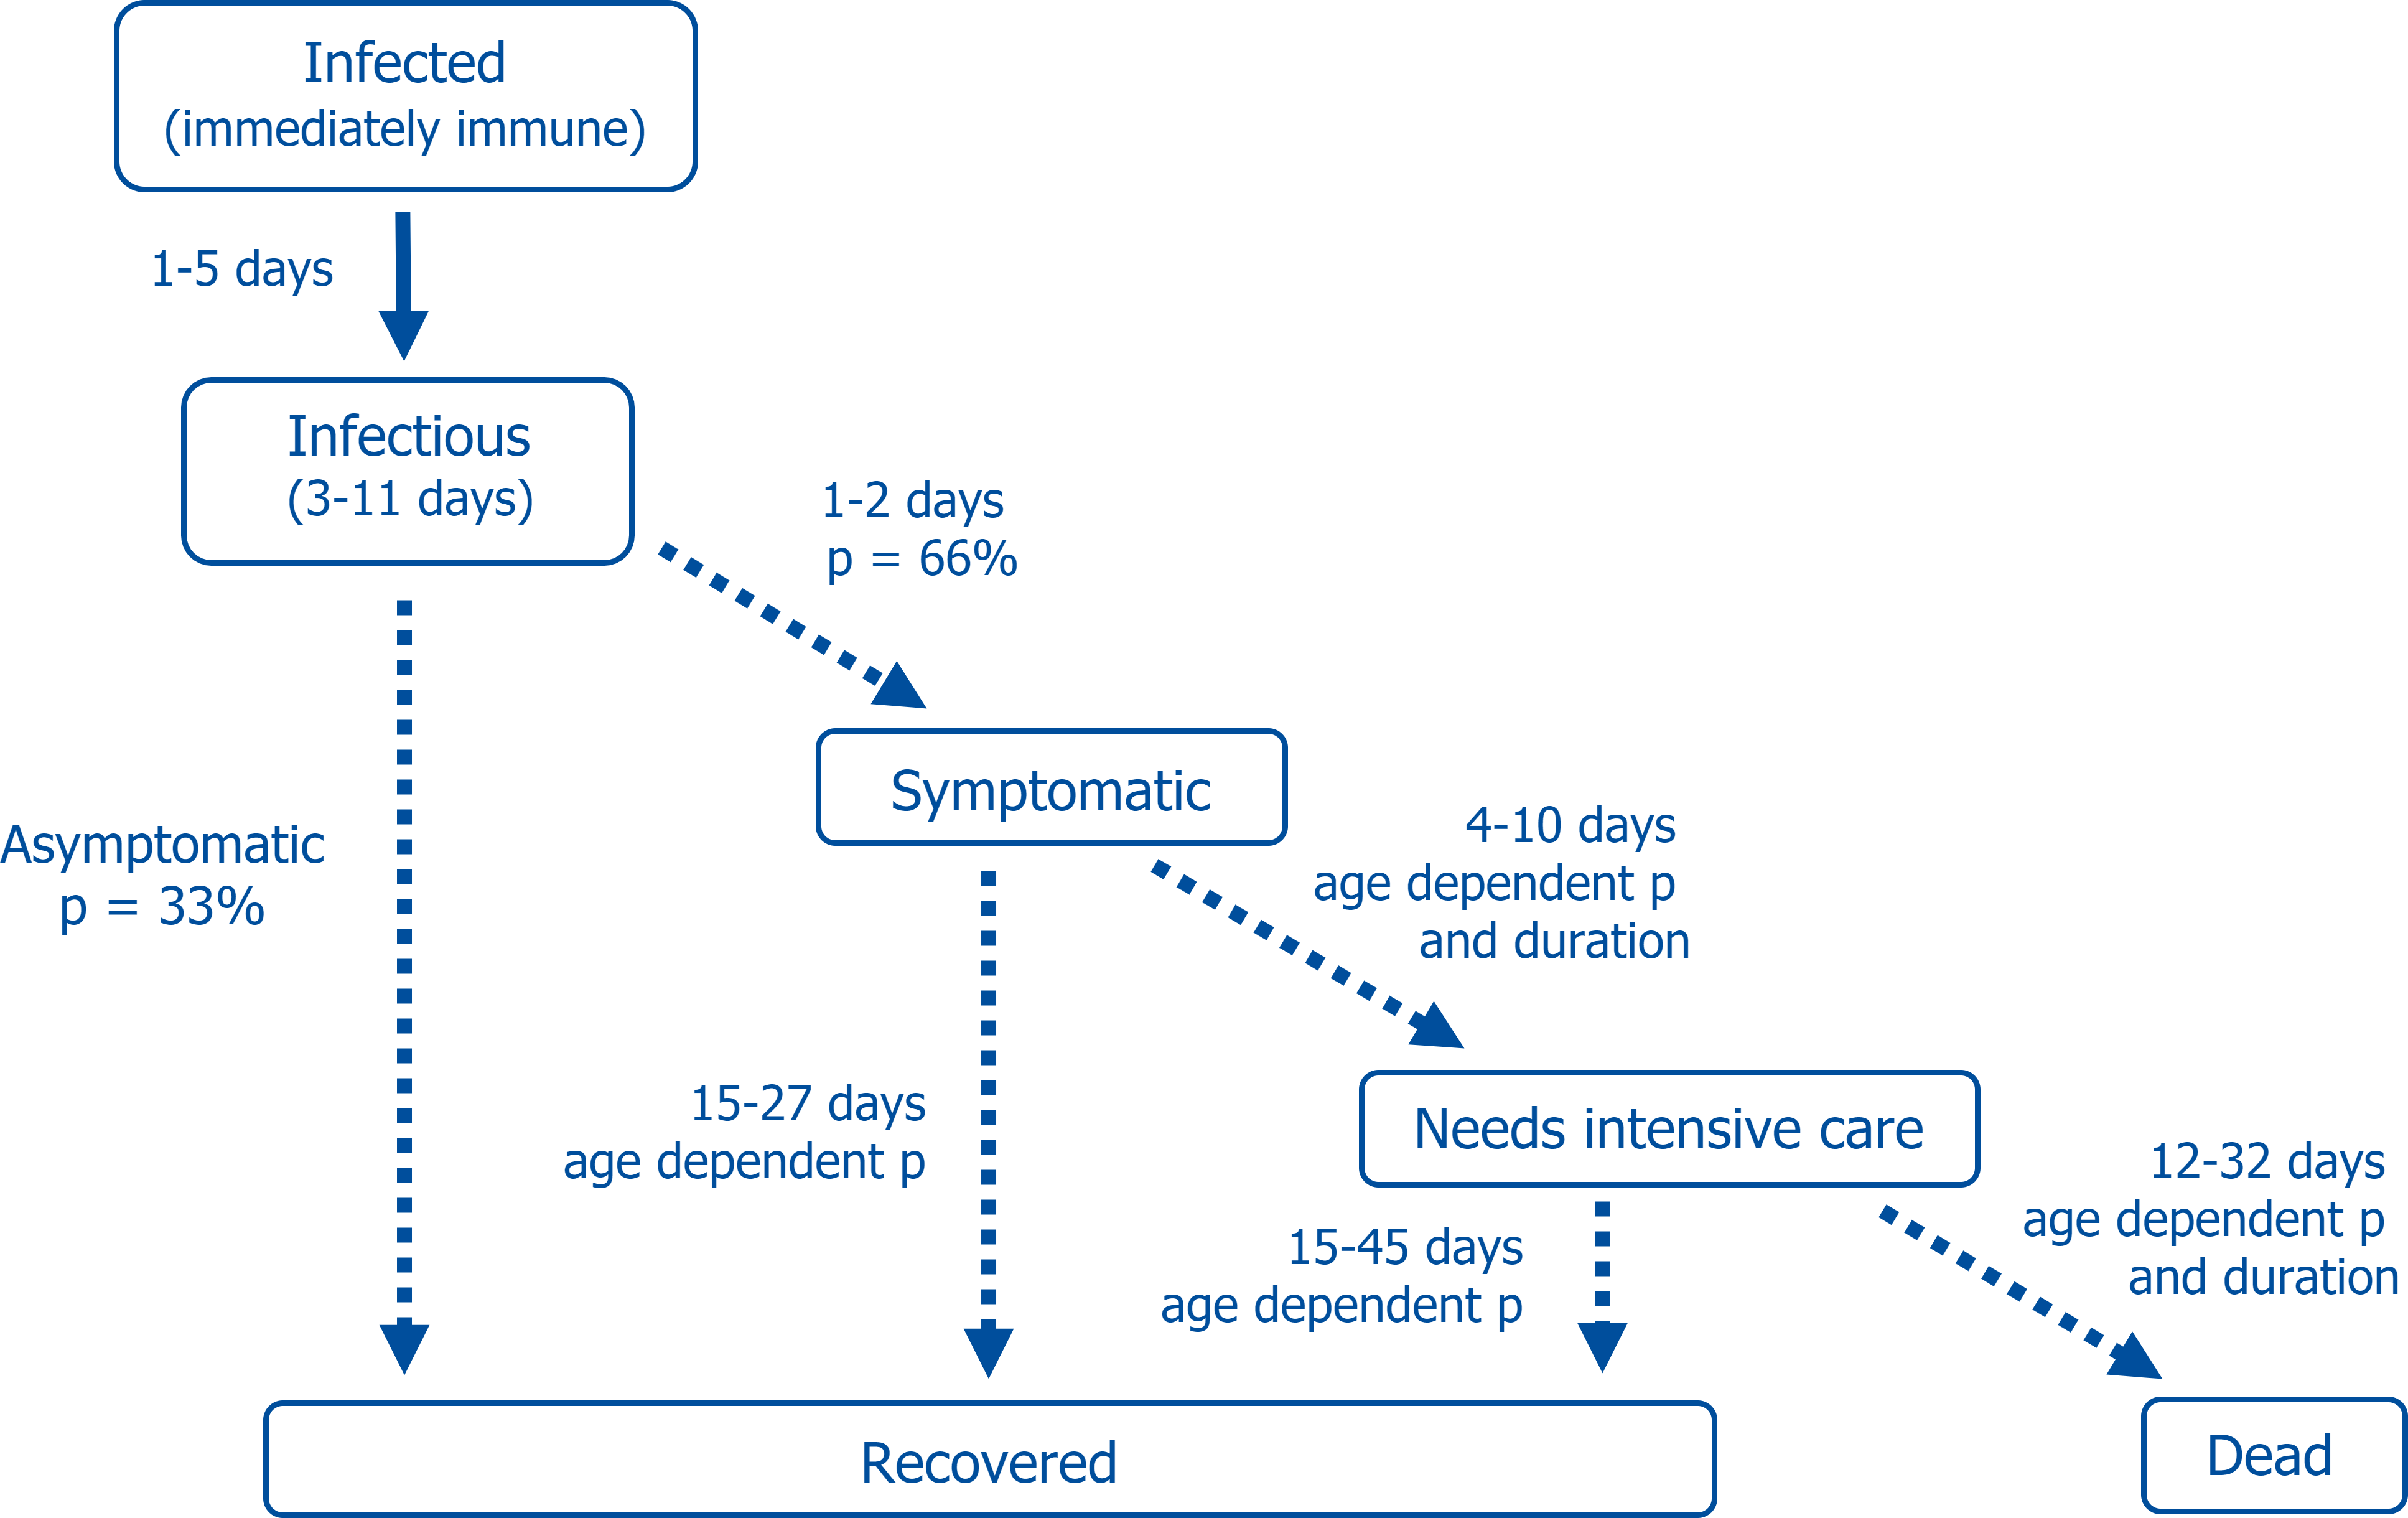
\includegraphics[width=\textwidth]{../figures/disease_progression.png}
    \caption{Course of Disease in the model}
    \label{fig:course_of_disease}
\end{figure}

First, infected individuals will become infectious after one to five days. About one third of people stays asymptomatic. The rest develops symptoms about one to two days after they become infectious. Modeling asymptomatic and pre-symptomatic cases is important because those people do not reduce their contacts or demand a test and can potentially infect many other people \citep{Donsimoni2020}.

A small share of symptomatic people will develop strong symptoms that require intensive care. The exact share and time span is age-dependent. An age-dependent share of intensive care unit (ICU) patients will die after spending up to 32 days in intensive care. Moreover, if the ICU capacity was reached, all patients who require intensive care but do not receive it die.

It would be easy to make the course of disease even more fine-grained. For example, we could model people who require hospitalization but not intensive care. So far we opted against that because only the ICU capacity might become a bottleneck in Germany.

We allow the progression of the disease to be stochastic in two ways: Firstly, state changes only occur with a certain probability (e.g. only a fraction of infected individuals develops symptoms). Secondly, the number of periods for which an individual remains in a state is drawn randomly. The parameters that govern these processes are taken from the literature. They can vary with the age of an individual.

Detailed information on the calibration of the disease parameters is available as part of our \href{https://sid-dev.readthedocs.io/en/latest/reference_guides/epi_params.html}{online documentation}.


\subsection{Testing} % (fold)
\label{sub:testing}

Having a realistic model of PCR and rapid tests is crucial for two reasons: Firstly, only
via a testing model can the simulated infections from the model be made comparable to
official case numbers. Secondly, individuals with undetected or not yet detected
infections are an important driver of the pandemic.

In principle, our modeling approach is flexible enough to incorporate mechanistic test
demand, allocation and processing models. However, there is not enough data available to
calibrate such a mechanistic model.

Therefore, we build a simpler model of PCR and rapid tests that can be calibrated with
available data on test demand and availability and -- nevertheless
-- can produce a share of undetected cases that varies over time and across age groups
and agrees with other estimates over the time periods where they are available.

PCR tests are modeled since the beginning of the simulation and determine whether a
infection is officially recorded. Rapid tests are only added at the beginning of 2021.
Positive rapid tests do not enter official case numbers directly, but most people with a
positive rapid tests demand a confirmatory PCR test. However, positive rapid tests can
have a strong effect on the infection dynamics because they trigger contact reductions
and additional rapid tests.

During 2020 people can demand PCR tests either because they have symptoms or randomly.
The probability that a PCR test is performed in each of the two situations depends on the
number of new infections and the number of available tests. Thus, it varies strongly over
time and is unknown.

To distribute the correct number of PCR tests among symptomatic and asymptomatic
infections without knowing explicit test demand probabilities, we use the following
approach: First, we calculate the total number of positive PCR tests by multiplying the
number of newly infected individuals with an estimate of the share of detected cases
from the Dunkelzifferradar project \citep{Dunkelzifferradar2020}. Next, we determine how
many of these tests should go to symptomatic and asymptomatic individuals from data by
the RKI \citep{ARS2020}. Then, we sample the individuals to which those tests
are allocated from the pools of symptomatic and asymptomatic infected but not yet tested
individuals.

Sampling uniformly from the pool of symptomatic individuals ensures that age groups who
are more likely to develop symptoms are also more likely to receive tests. Thus, the
share of detected cases is much higher for the elderly than for children in time periods
where many tests are done because of symptoms.

At the beginning of 2021, two challenges arise: Firstly, the externally estimated share
of detected cases from Dunkelzifferradar project \citep{Dunkelzifferradar2020} can no
longer be used because it is based on the case fatality rate which changes drastically
due to vaccinations. Secondly, rapid tests become available at a large scale.

We solve the first challenge by assuming that the share of detected cases would have 
remained at the level it reached before Christmas if rapid tests had not become 
available. While this is only an approximation to reality, changes in the share of 
detected cases that would have happened without rapid tests are very likely to be small 
compared to the changes caused by rapid tests. In addition, the number of PCR tests per 
1000 remains in the same 1.5 to 2.5 window without a visible trend over our estimation 
period \citep{owid_n_pcr_tests} which is in line with less than 0.08\% of the 
population receiving a positive rapid test on any given day in our model.

The second challenge is solved by mechanistic rapid test demand models for the
workplace, schools and by private individuals. The calibration of these models is
described in Section~\ref{subsec:rapid_test_demand}.
Figure~\ref{fig:antigen_tests_vaccinations} shows that the number of performed rapid
tests in the model fits the empirical data well (where empirical data is available).

In contrast to PCR tests, rapid tests are not perfect and can be falsely positive or
falsely negative. While the specificity of rapid tests is calibrated at 99.4\%
\citep{Bruemmer2021}, their sensitivity strongly depends on the timing of the rapid test
relative to the start of infectiousness \citep{Smith2021}. Before the onset of
infectiousness the sensitivity is very low (35\%). On the first day of infectiousness it
is much higher (88\%) but still lower than during the remaining infectious period (92\%).
After infectiousness stops, the sensitivity drops to 50\%.

Modeling the diagnostic gap before and at the beginning of infectiousness is very
important to address concerns that rapid tests are too unreliable to serve as screening
devices.

We do not distinguish between self administered rapid tests and those that are
administered by medical personnel. While there were concerns that self administered
tests are less reliable, a recent study has found no basis for this concern
\citep{Lindner2020}.

While rapid tests do not directly enter official case numbers, 82\%
($\chi_{confirmation}$) of positively tested individuals seek a PCR test
\citep{Betsch2021}. Importantly, those PCR tests are made in addition to the tests that
would have been done otherwise. Section~\ref{subsec:results_share_known_cases} discusses
the effect of rapid tests on the share of detected cases.



\subsection{Initial Conditions} % (fold)
\label{sub:initial_conditions}

Consider a situation where you want to start a simulation with the beginning set amidst
the pandemic. It means that several thousands of individuals should already have
recovered from the disease, be infectious, symptomatic or in intensive care at the start
of your simulation. Additionally, the sample of infectious people who will determine the
course of the pandemic in the following periods is likely not representative of the whole
population because of differences in behavior (number of contacts, assortativity), past
policies (school closures), etc.. The distribution of health states in the population at
the beginning of the simulation is called initial conditions.

To come up with realistic initial conditions, we match reported infections from official
data to simulated individuals by age group and county. We use one month of data to
generate initial conditions with in all possible health states. Meanwhile health states
evolve until the beginning of the simulation period without simulating infections by
contacts. We also correct reported infections for a reporting lag and scale them up by
the share of detected cases to arrive at the true number of infections.

% subsection initial_conditions (end)



    \section{Additional Results}
\label{sec:additional_results}

\subsection{Simulated vs. Empirical Data}
\label{subsec:new_cases_fit}

This compares simulated data from our model with empirical data from Germany. We look at
observed infections, fatality rates, the spread of the B117 mutation, vaccinations and
rapid test demands. Where available we do not only look at aggregated statistics but also
analyze the model fit for age groups.\comment[id=J]{summarize the
fit}\comment[id=HM]{Also need to show simulated total infections somewhere. So far only
ever shown for 2021.}


\begin{figure}[ht]
  \centering
  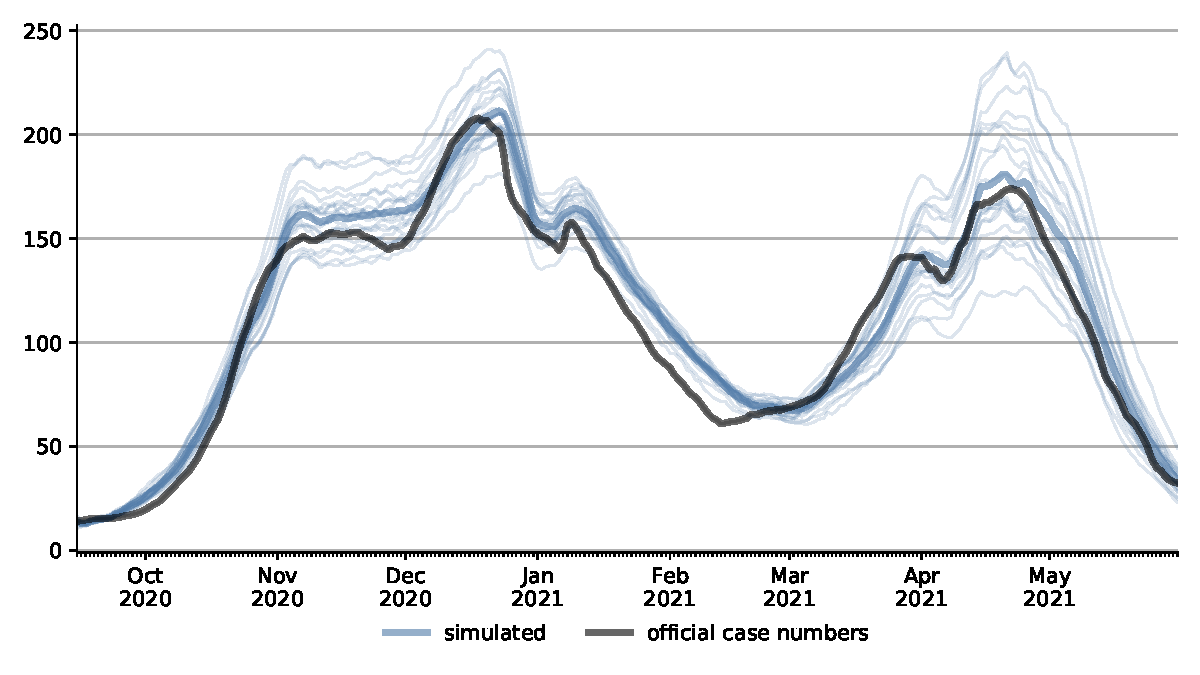
\includegraphics[width=\textwidth]{../figures/results/figures/scenario_comparisons/combined_fit/full_new_known_case_with_single_runs}
  \caption{Simulated and Empirical Infections}
  \figurenotes{The figure shows the weekly incidence rates per 100,000 people for the
  reported versus the simulated infections rates.}
  \label{fig:aggregated_fit2}
\end{figure}


\begin{figure}[ht]
  \centering
  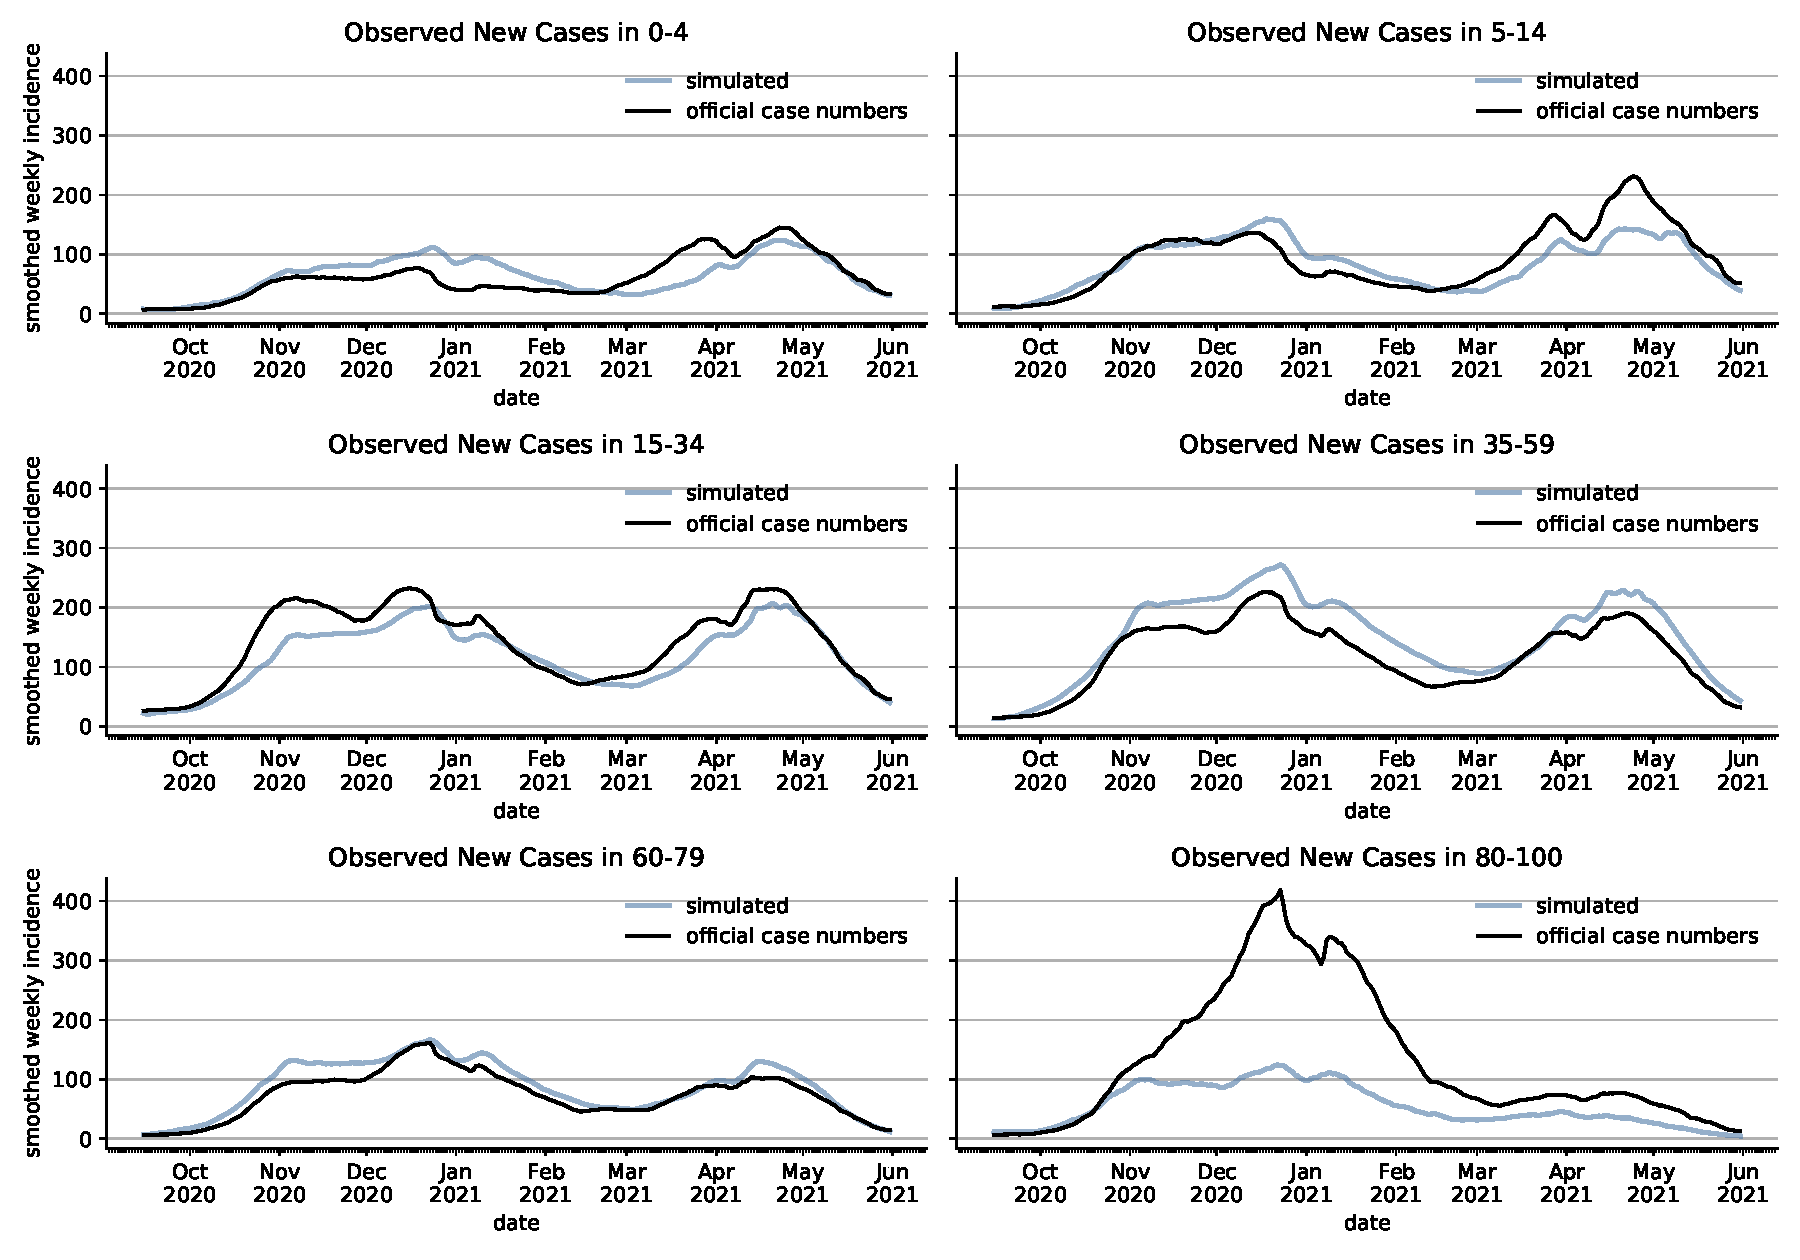
\includegraphics[width=\textwidth]{../figures/results/figures/incidences_by_group/age_group_rki/full_combined_baseline_new_known_case}
  \caption{Simulated and Empirical Infections by Age Group}
  \figurenotes{The figure shows the weekly incidence rates per 100,000 people for the
  reported versus the simulated infections rates for different age groups.}
  \label{fig:age_group_fit}
\end{figure}


\begin{figure}[ht]
  \centering
  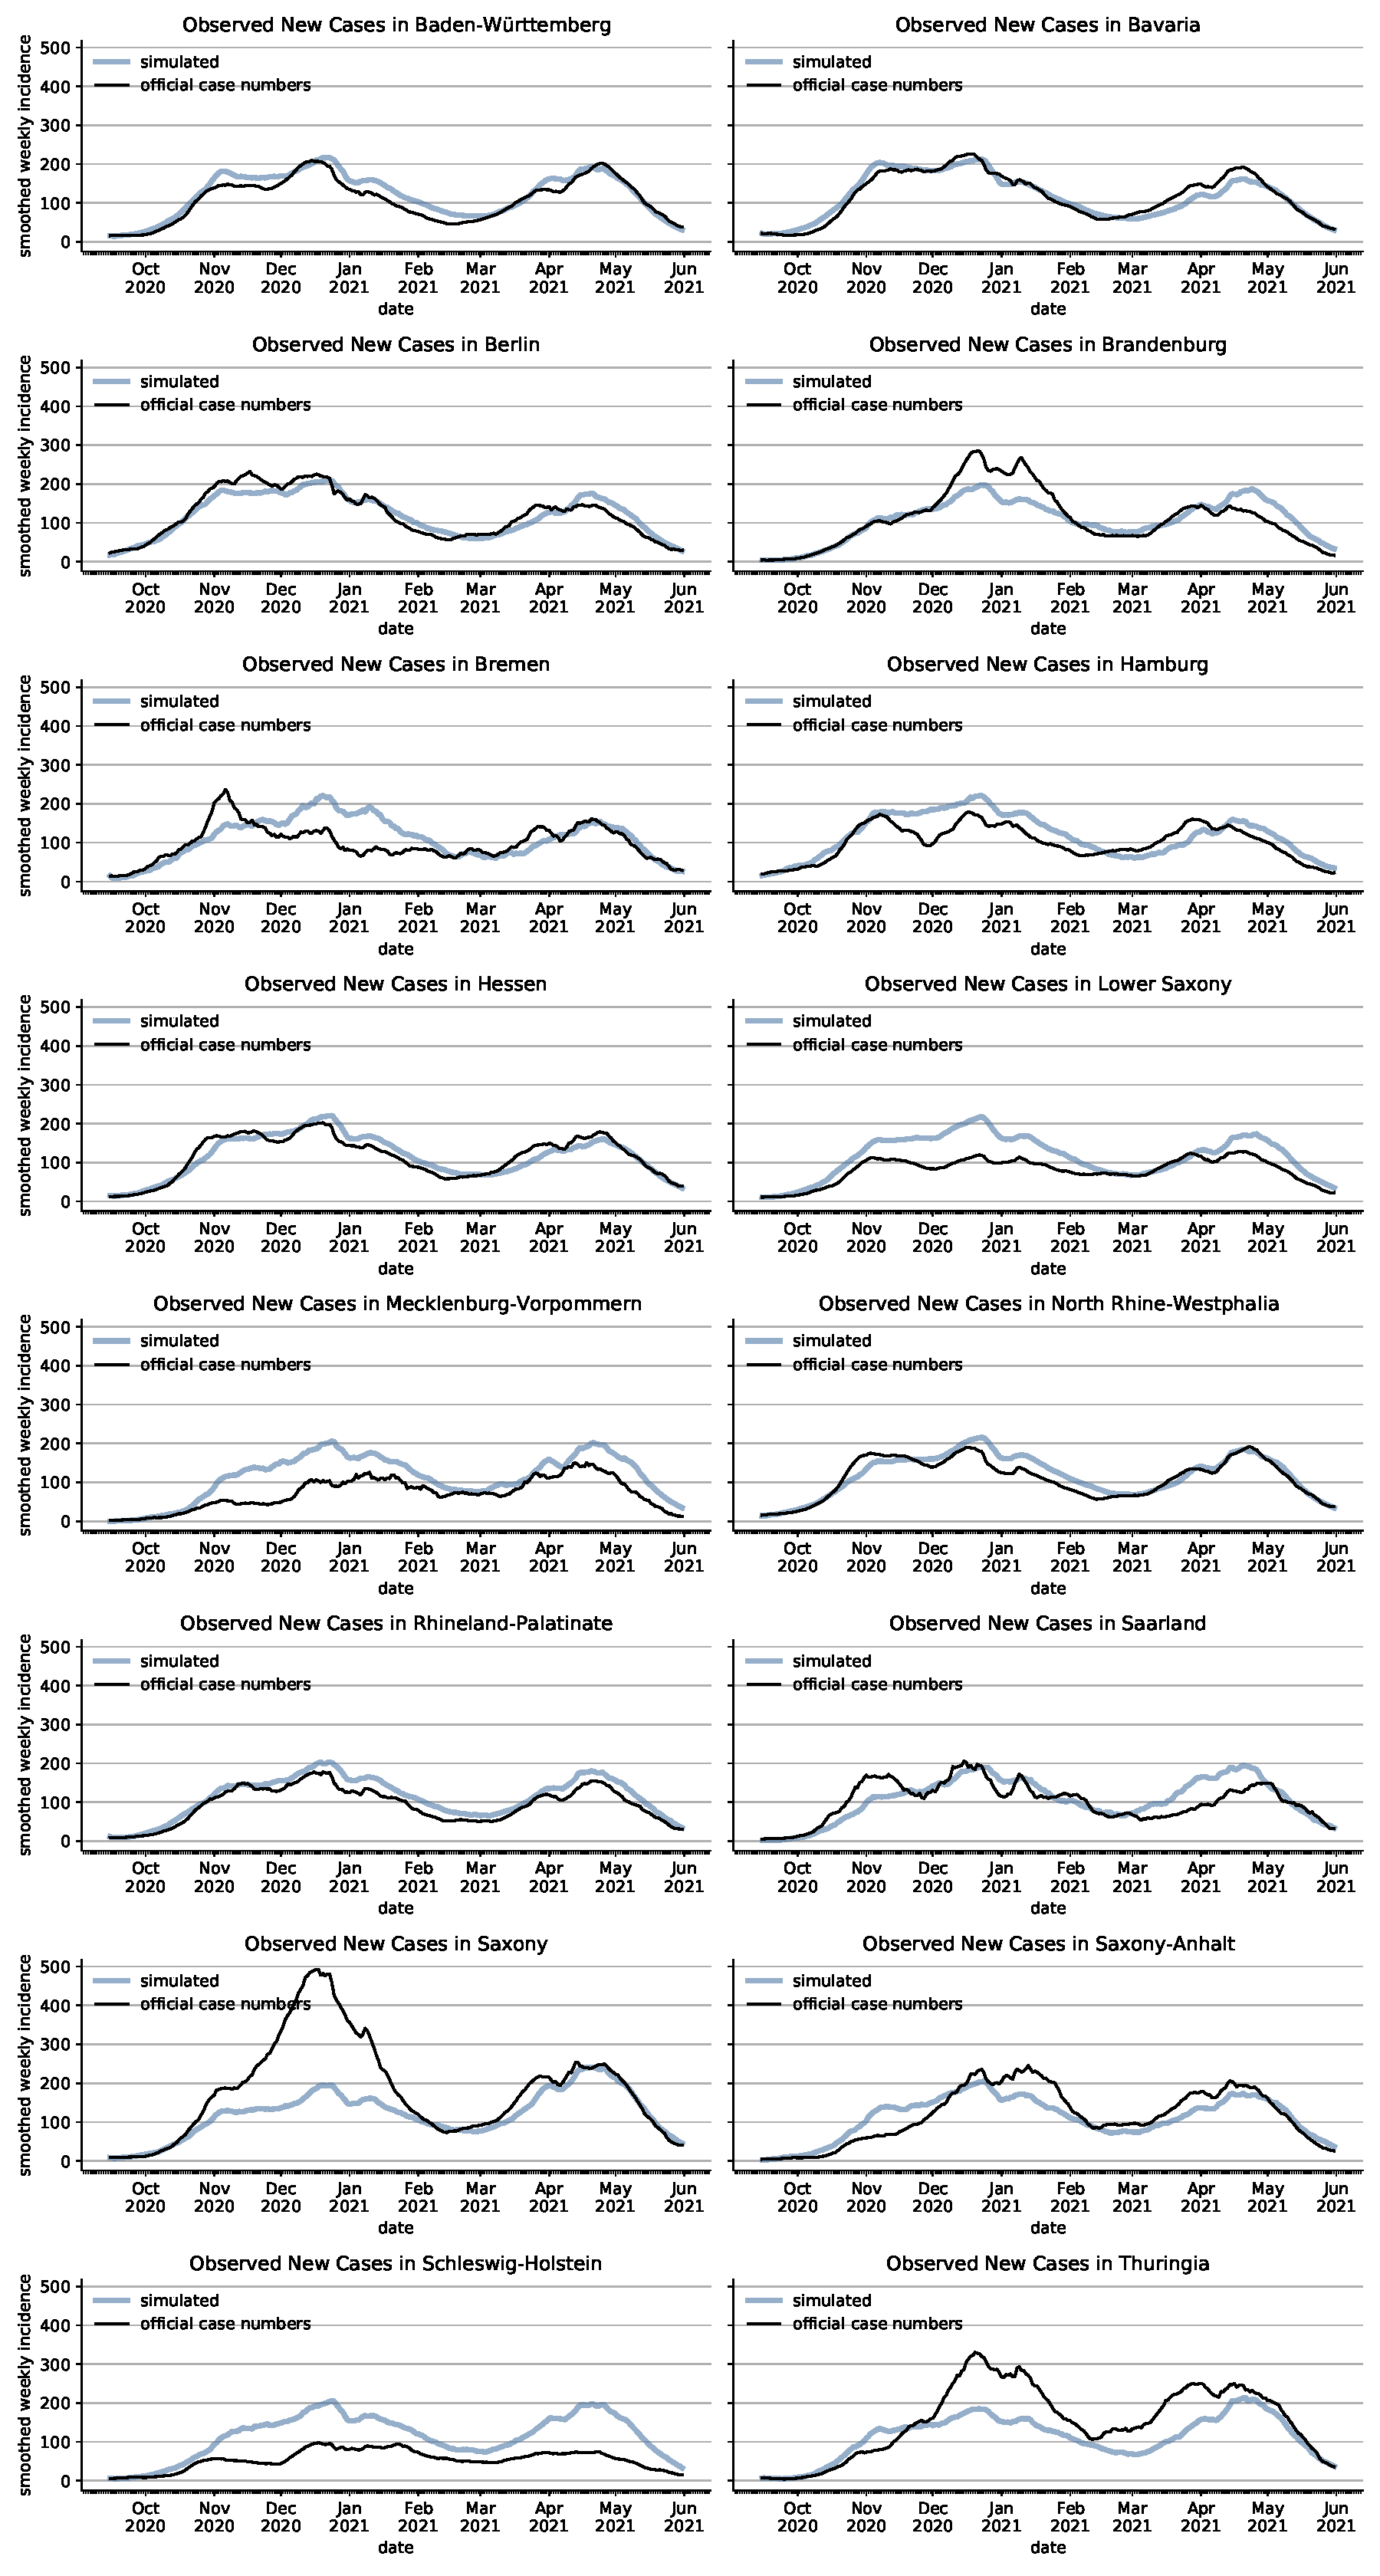
\includegraphics[width=\textwidth]{../figures/results/figures/incidences_by_group/state/full_combined_baseline_new_known_case}
  \caption{Simulated and Empirical Infections by Federal State}
  \figurenotes{The figure shows the weekly incidence rates per 100,000 people for the
  reported versus the simulated infections rates for different federal states.}
  \label{fig:state_fit}
\end{figure}


\FloatBarrier


\subsection{Share of Cases that are Detected  \comment[id=K]{Figure notes missing}}
\label{subsec:appendix_share_known_cases}

\begin{figure}[ht]
  \centering
  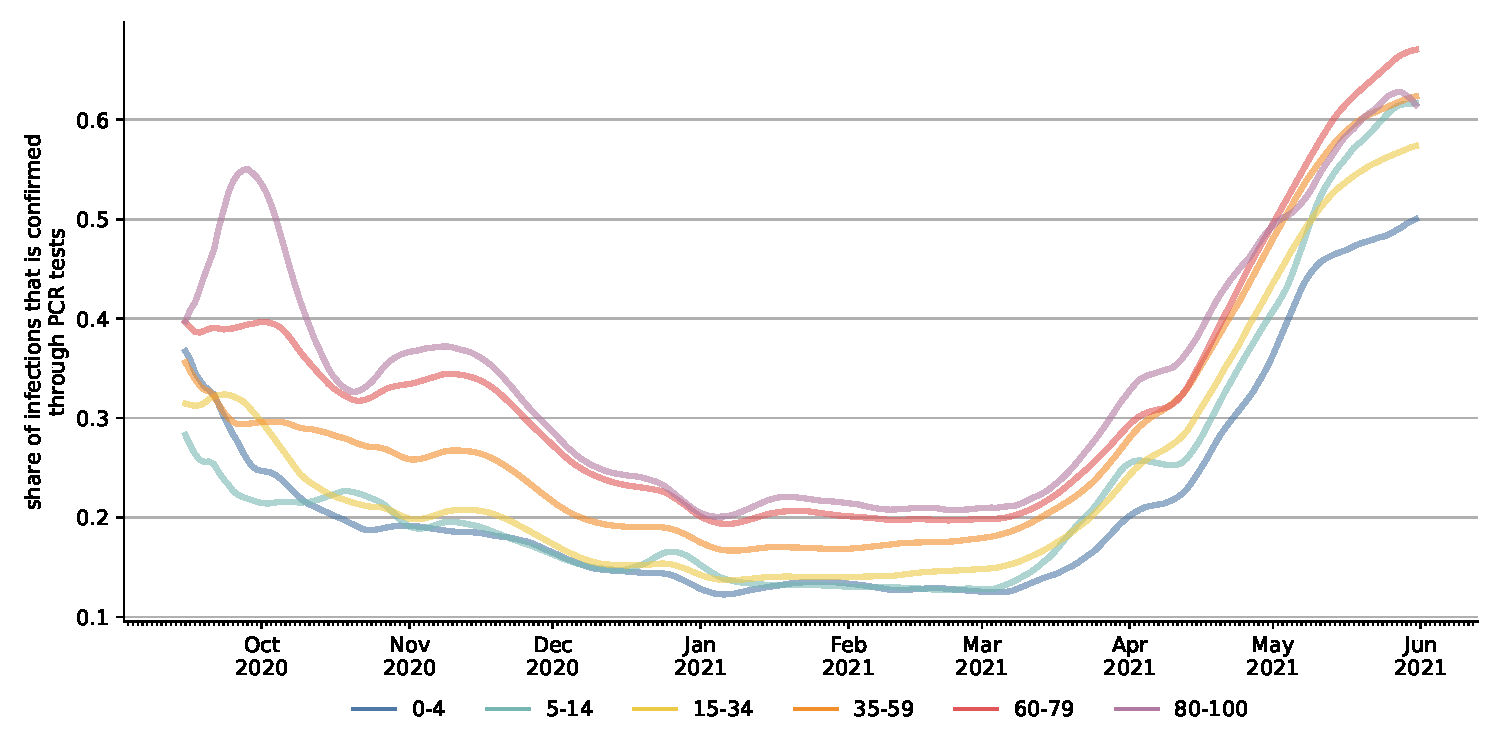
\includegraphics[width=\textwidth]{../figures/results/figures/share_known_cases/full_combined_baseline_by_age_group_rki}
  \caption{Share of Detected Cases by Age Group in the Main Prediction}
  \label{fig:share_known_cases_by_age_group}
  \floatfoot{\noindent}
\end{figure}

It's noteworthy that the share of detected cases increases rapidly in May for the five to
fourteen year olds. This is a direct result of the mandatory tests in
school.

\subsection{Rapid Tests \comment[id=K]{The figures will likely change layout later}}
\label{subsec:appendix_rapid_tests}

\begin{figure}[ht]
  \centering
  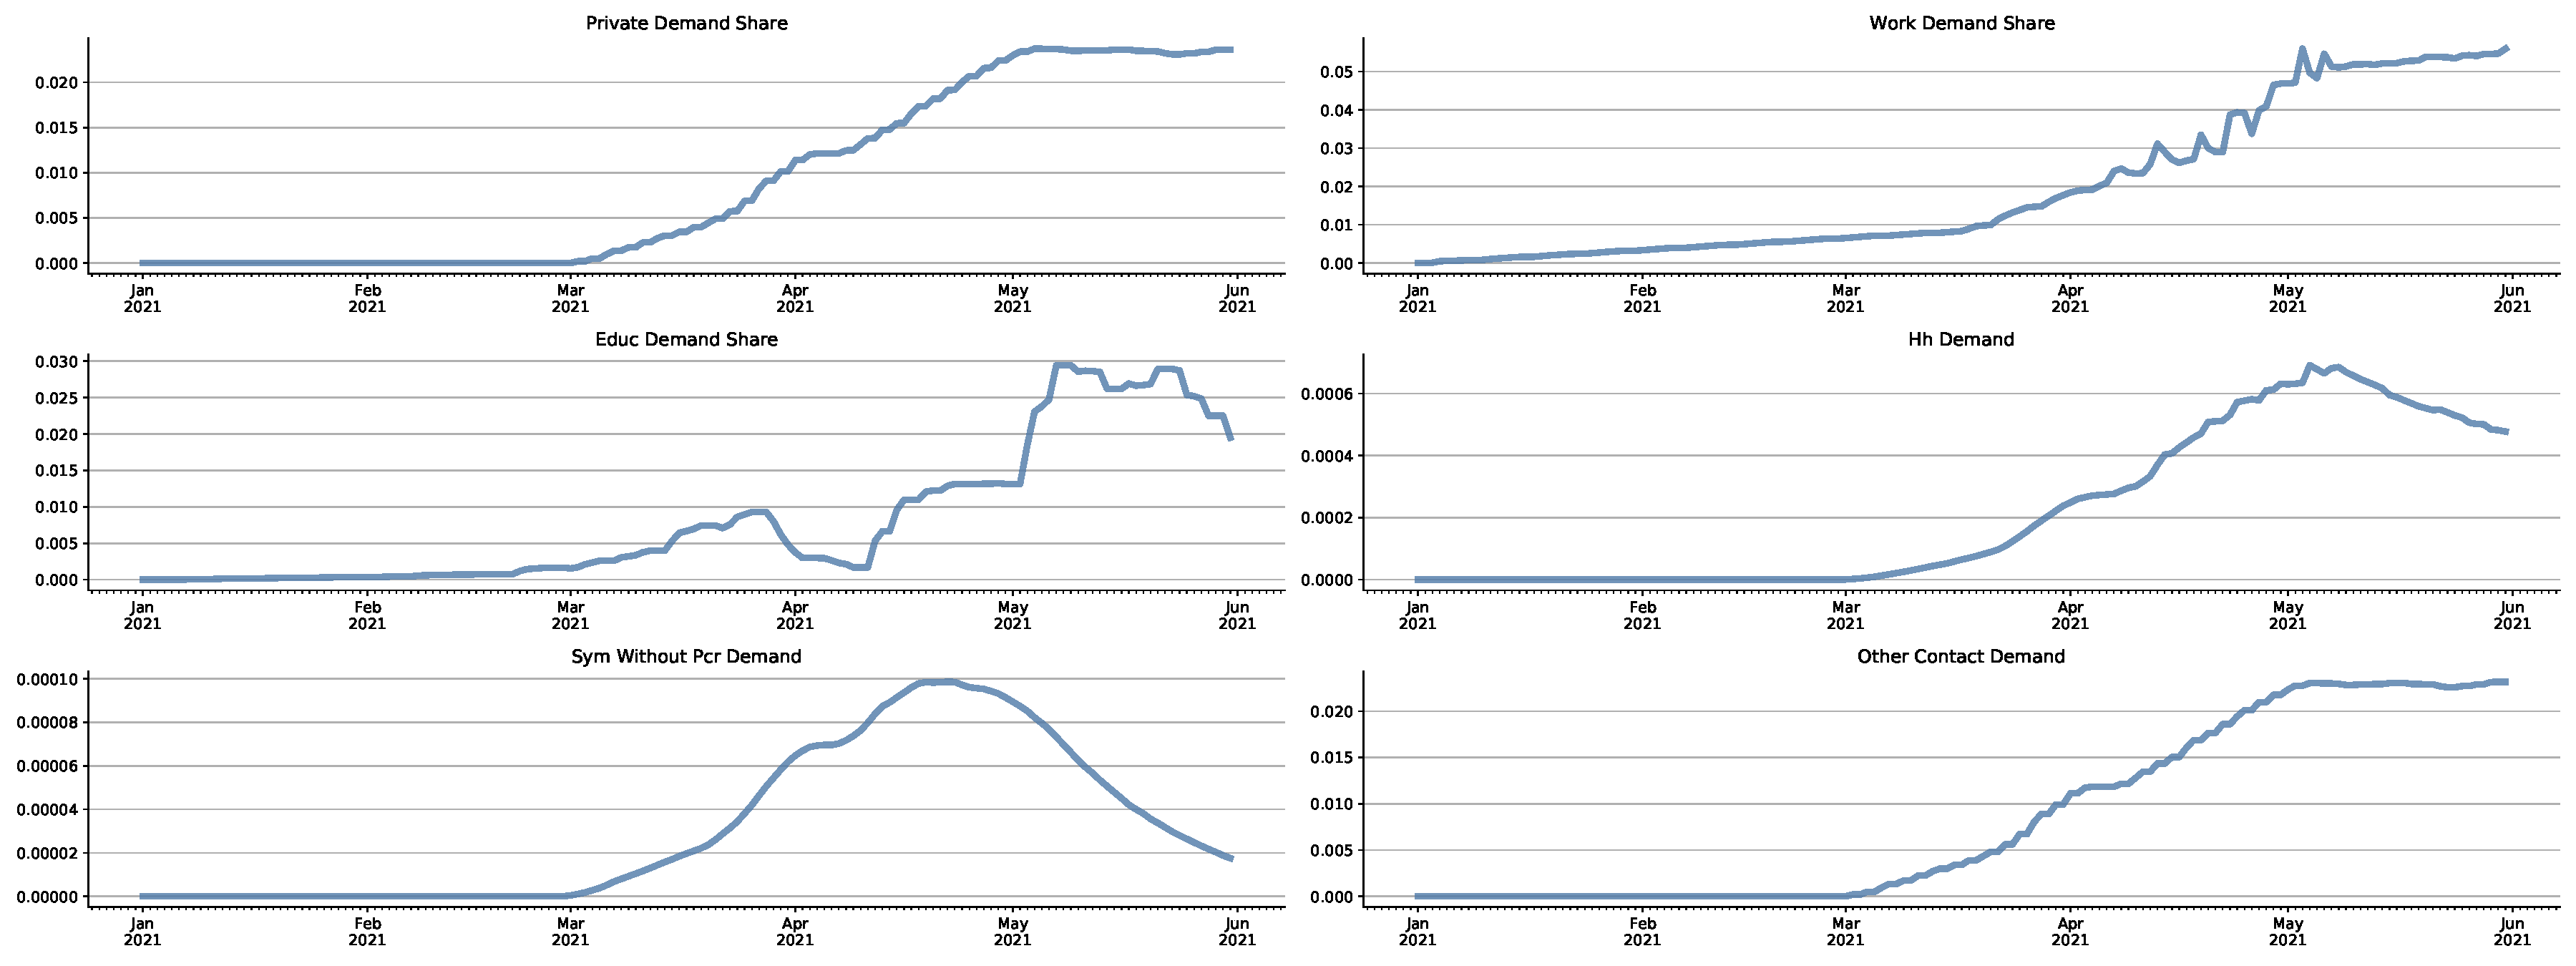
\includegraphics[width=\textwidth]{../figures/results/figures/rapid_test_statistics/demand_shares}
  \caption{Share of the Population Demanding a Rapid Test for a Particular Reason}
  \label{fig:rapid_tests_by_reason}
  \floatfoot{\noindent Note that the lower three (household demand, symptomatic without
  PCR demand and other contact demand together form the private demand category. Also
  note that these do not add up to the total share of demanded rapid tests as individuals
  may have more than one reason to demand a rapid test on any given day. }
\end{figure}

\begin{figure}[ht]
  \centering
  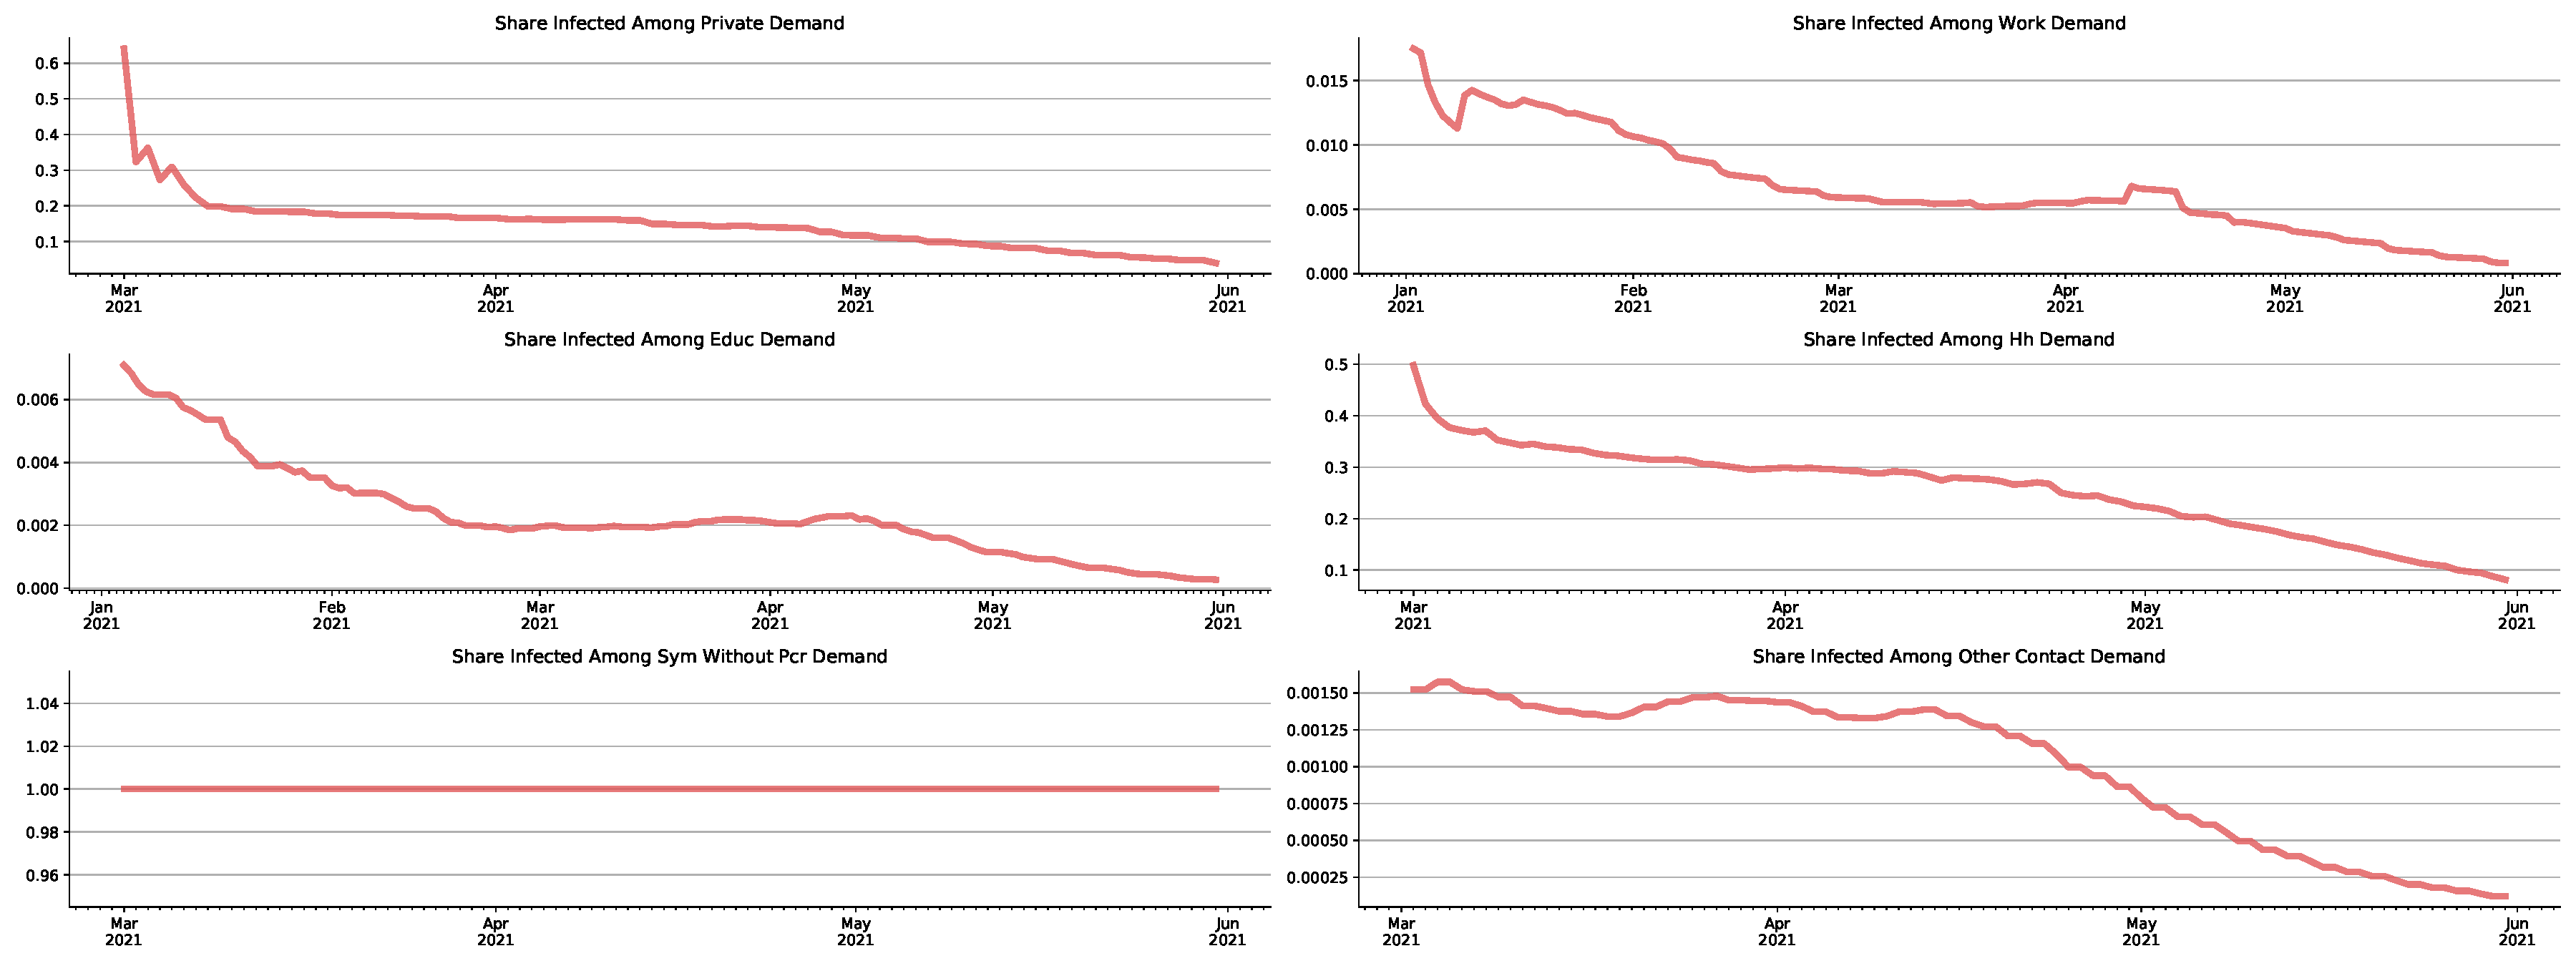
\includegraphics[width=\textwidth]{../figures/results/figures/rapid_test_statistics/share_infected_among_demand}
  \caption{Share of individuals who Demand a Rapid Test for a Particular Reason that are Actually Infected}
  \label{fig:share_of_rapid_tests_by_reason_by_infected}
  \floatfoot{\noindent Note that the lower three (household demand, symptomatic without
  PCR demand and other contact demand together form the private demand category. Also
  note that this is not the same as individuals getting a positive rapid test. The
  sensitivity is quite low before individuals become infectious. Therefore, if
  individuals are still in the latent period of their infection they are likely to get a
  false positive rapid test.}
\end{figure}

\FloatBarrier


\subsection{Scenarios}
\label{subsec:appendix_scenarios}

This is the results section.\comment[id=K]{The results can be found in `figures/results`.
This includes both figures and tables for lookup of numbers and summary tables.}


\begin{figure}[ht]
  \centering
  \begin{subfigure}{.6\textwidth}
    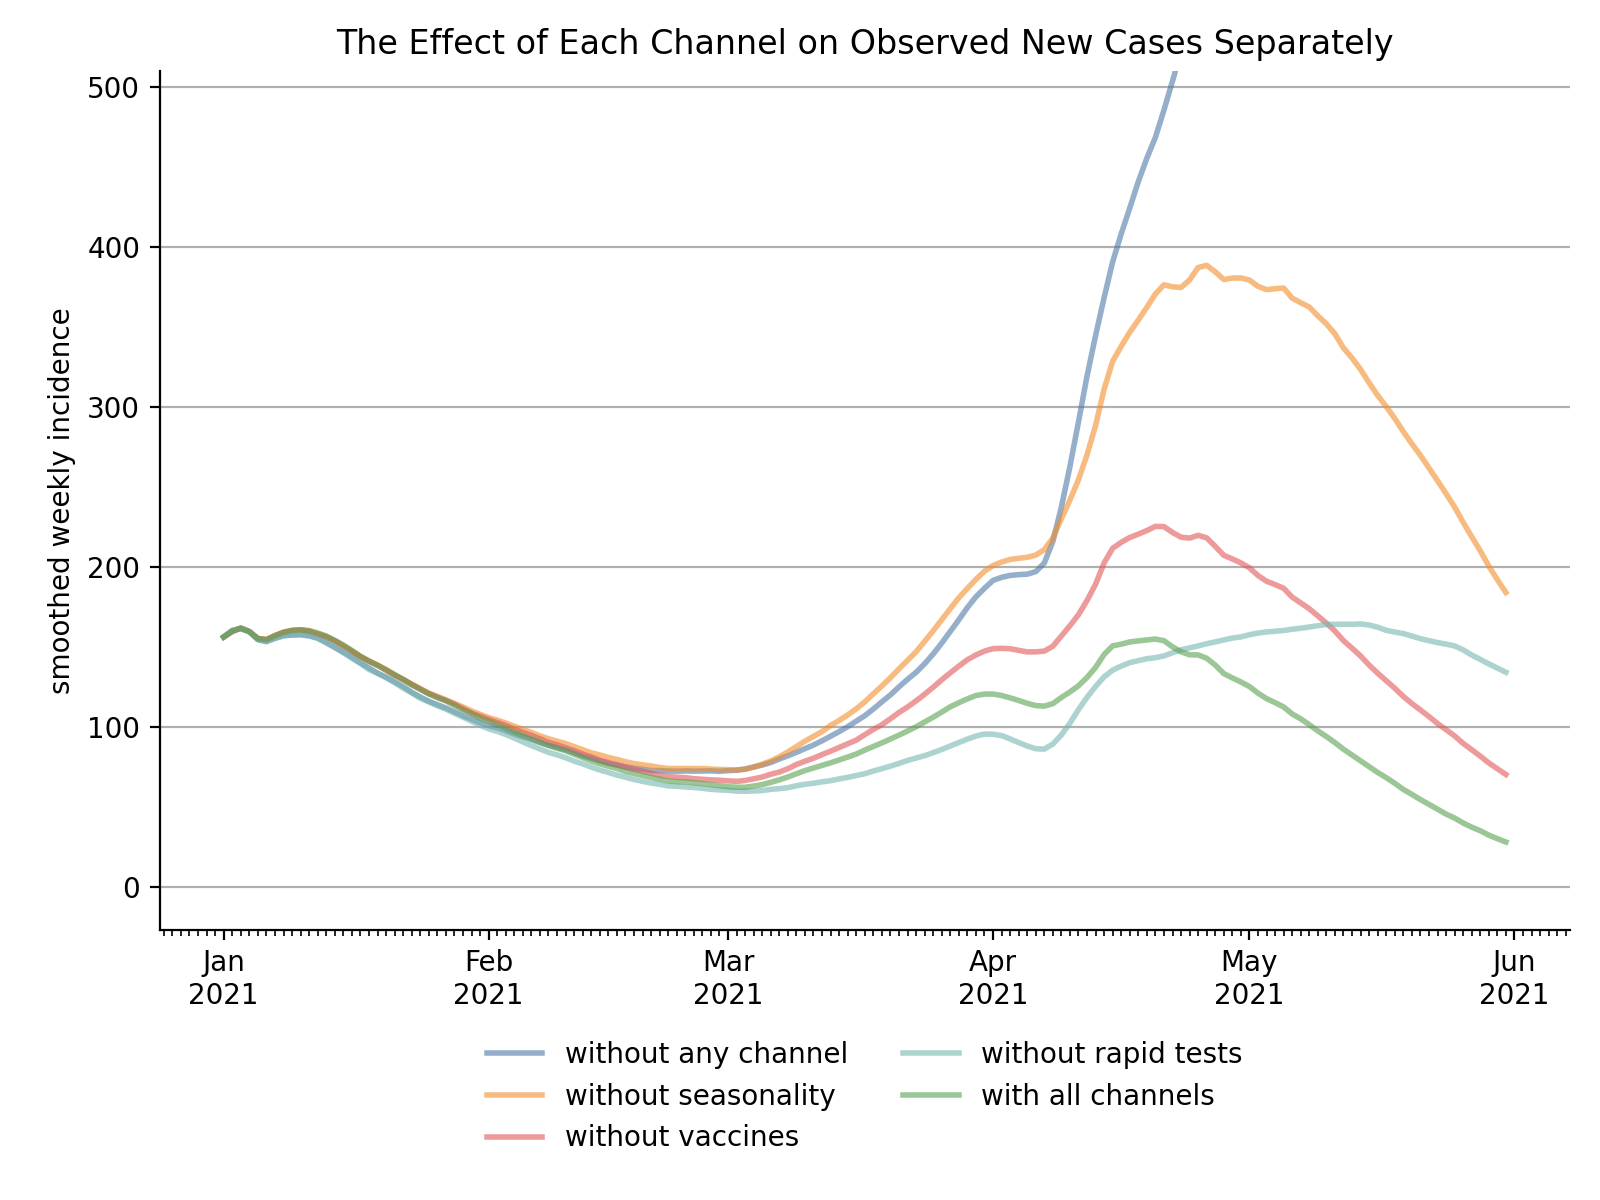
\includegraphics[width=0.9 \textwidth]{../figures/results/figures/scenario_comparisons/one_off_and_combined/full_new_known_case_cropped}
  \end{subfigure}%
  \begin{subfigure}{.6\textwidth}
    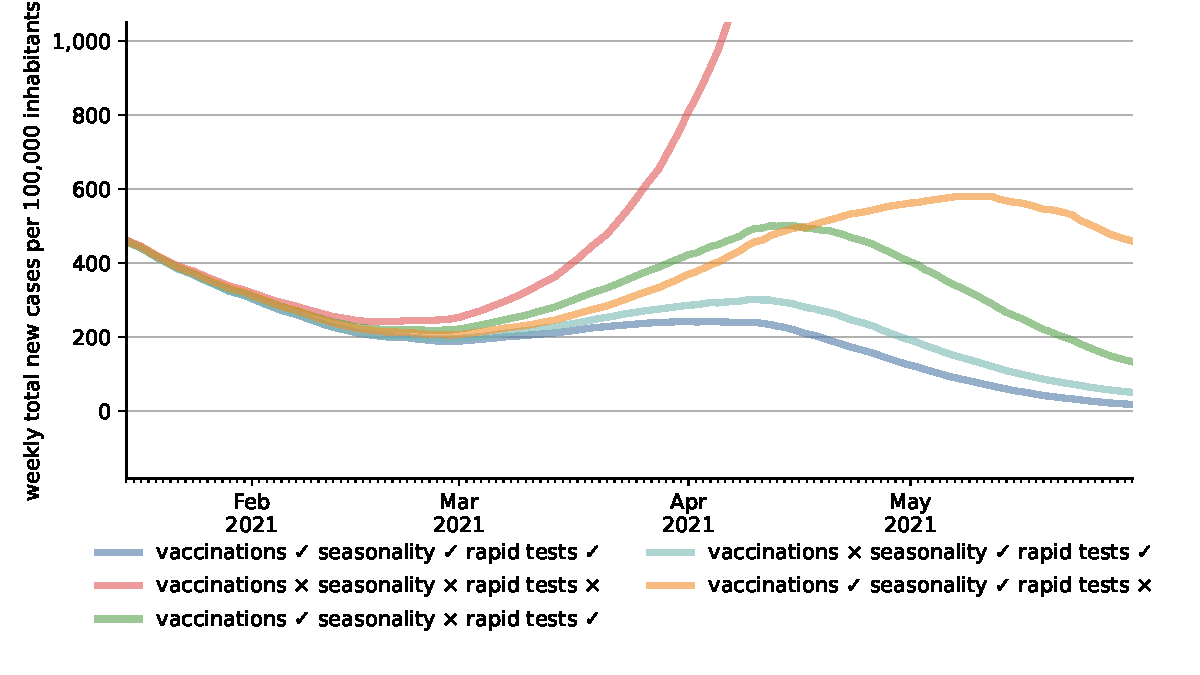
\includegraphics[width=0.9 \textwidth]{../figures/results/figures/scenario_comparisons/one_off_and_combined/full_newly_infected_cropped}
  \end{subfigure}
  \caption{The Effect of Policies on Observed and Unobserved Cases}
  \label{fig:explain_decline}
  \figurenotes{\ldots}
\end{figure}



\begin{figure}[ht]
  \centering
  \begin{subfigure}{.6\textwidth}
    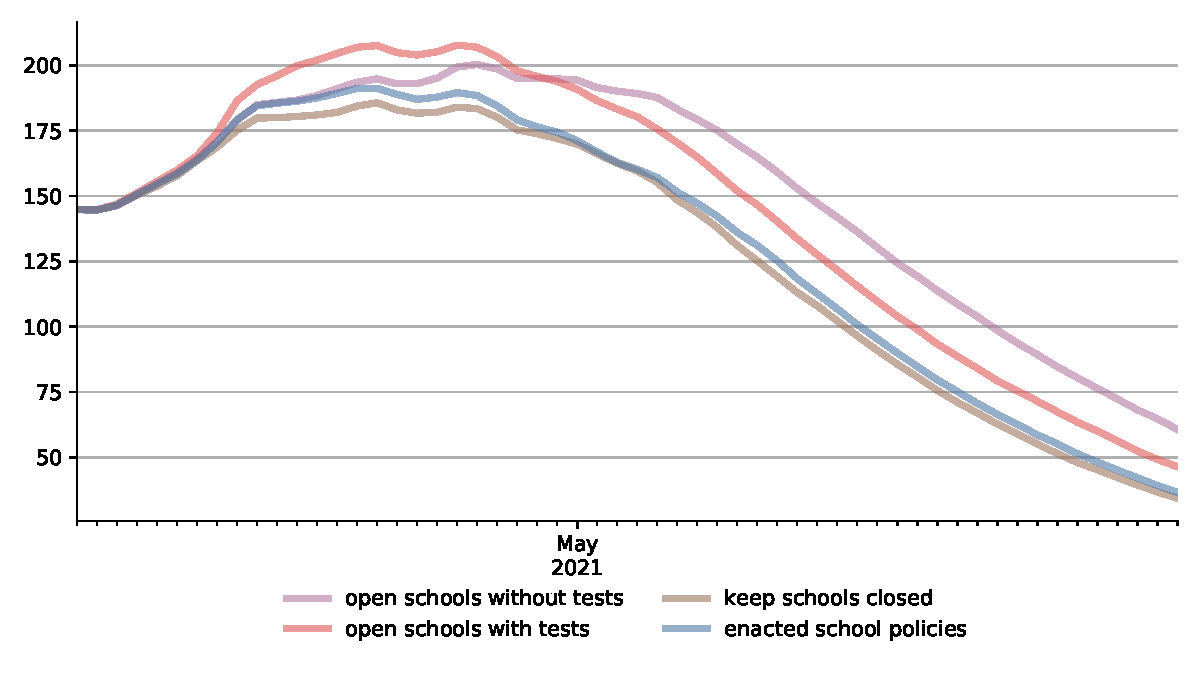
\includegraphics[width=0.9 \textwidth]{../figures/results/figures/scenario_comparisons/school_scenarios/full_new_known_case}
  \end{subfigure}%
  \begin{subfigure}{.6\textwidth}
    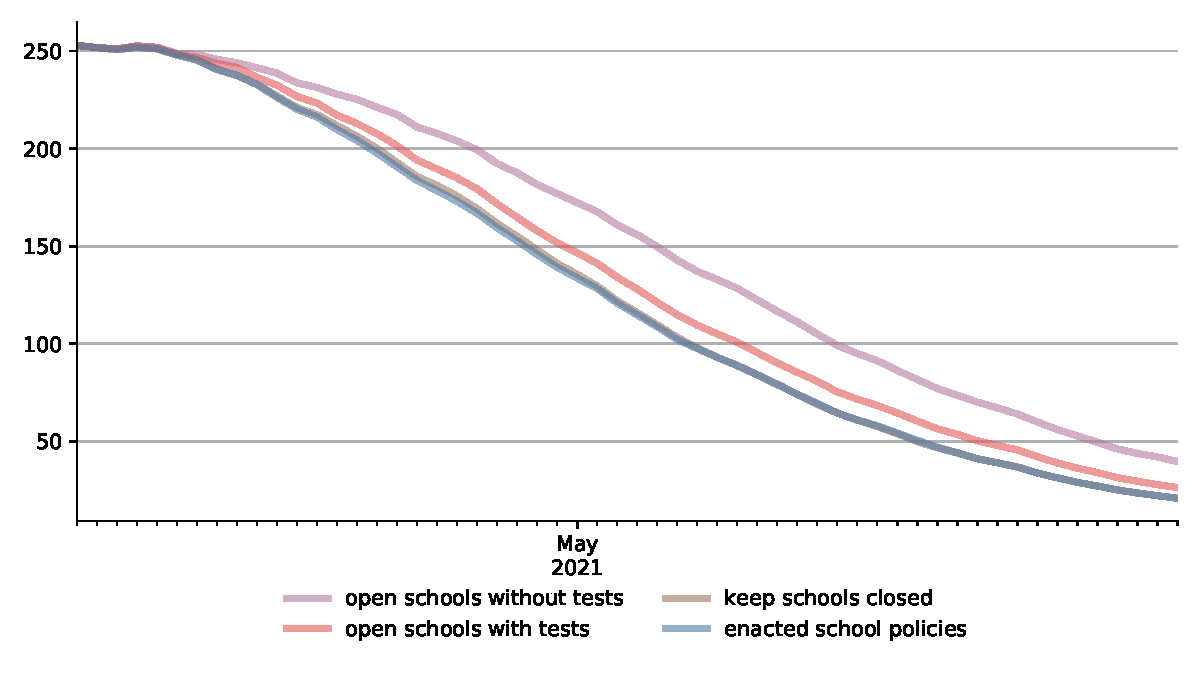
\includegraphics[width=0.9 \textwidth]{../figures/results/figures/scenario_comparisons/school_scenarios/full_newly_infected}
  \end{subfigure}
  \caption{The Effect of Different School Scenarios on Observed and Unobserved Cases}
  \label{fig:school_scenarios_detailed}
\end{figure}


\FloatBarrier

\begin{tabular}{lr}
\toprule
{} &  predicted total infections among 5-14 year olds from Easter until 2021-05-31 \\
scenario                               &                                                                               \\
\midrule
 educ open after easter  without tests &                                             775324 \\
 educ open after easter  with tests    &                                             604078 \\
 close educ after easter               &                                             469274 \\
 baseline                              &                                             478080 \\
\bottomrule
\end{tabular}


\FloatBarrier


\subsection{Shapley Value} % (fold)
\label{sub:shapley_value}

We decompose the effects of different NPIs and seasonality on the infection rates with
Shapley values. Shapley values \citep{Shapley2016} are a concept in game theory to
divide payoffs between a coalition of players. It allows to assign a single value to the
contribution of an NPI or seasonality which takes into account substitutional and
complementary effects with other factors.

More formally, define a coalitional game with $N$ players and a super-additive function
$\nu$ which maps subsets of $N$ to the real numbers. The function $\nu$ is also called
the characteristic function and assigns a value to a coalition. Then, the Shapley value
$\phi$ for player $i$ is

\begin{align*}
    \phi_i(\nu) = \frac{1}{|N| !} \sum_{S \subseteq N \setminus \{i\}} |S| ! (|N| - |S| - 1)! (\nu(S \cup \{i\}) - \nu(S))
\end{align*}

The last term $(\nu(S \cup \{i\}) - \nu(S))$ is the marginal contribution of player $i$
minus the coalition without player $i$. Then, compute the sum of marginal contributions
over all subsets $S$ of $N$ which do not include player $i$. Each marginal contribution
has to be multiplied by all combinations of other players in $S$ which precede $i$ and
all possible combinations of remaining players which follow player $i$ in the coalition.
To arrive at the Shapley value for player $i$, divide the sum by the total number of
combinations.

The Shapley value has some properties.

\begin{description}
  \item[Efficiency] The sum of Shapley values is equal to the value of a coalition
  formed by all players.
  \item[Symmetry] The Shapley does not depend on the label of a player but only on its
  position in the characteristic function.
  \item[Linearity] The Shapley value depends linearly on the values from the
  characteristic function $\nu$.
  \item[Dummy Axiom] The Shapley value of a player who contributes nothing to any
  coalition is 0.
\end{description}

To produce Figure~\ref{fig:2021_scenarios_decomposition} and
Figure~\ref{fig:2021_scenarios_decomposition_tests}, we calculate the Shapley values of
each factor in the comparison on the cumulative number of saved infections between the
main scenario and the scenario without any of the factors for every day. Then, we divide
up the saved infections on a particular day according to the Shapley values for the same
day which yields the daily saved infections for each factor.


% subsection shapley_value (end)


    \printbibliography[heading=bibintoc]

    \end{refsection}
\end{appendices}

\end{document}
